\PassOptionsToPackage{dvipsnames}{xcolor}
\PassOptionsToPackage{unicode}{hyperref}
\PassOptionsToPackage{naturalnames}{hyperref}
\documentclass[aspectratio=169,10pt]{beamer}

% speaker notes
% open pdf in dual screen using pympress (https://github.com/Cimbali/pympress)
\setbeameroption{show notes on second screen=right}

% listings (should be loaded before csquotes)
\usepackage{minted}

% language and encoding
\usepackage[french]{babel}
\usepackage[T1]{fontenc}
\usepackage{csquotes}

% biblatex for references on slides
\usepackage[backend=biber]{biblatex}
\addbibresource{defense.bib}
% clean, short citations in footnotes (cf. https://tex.stackexchange.com/a/587604)
\renewbibmacro{in:}{}
% \AtEveryCitekey{\clearfield{journaltitle}}
\AtEveryCitekey{\clearfield{volume}}
\AtEveryCitekey{\clearfield{number}}
\AtEveryCitekey{\clearfield{booktitle}}
% \AtEveryCitekey{\clearfield{series}}
\AtEveryCitekey{\clearfield{pages}}
\AtEveryCitekey{\clearfield{month}}
\AtEveryCitekey{\clearlist{publisher}}
\AtEveryCitekey{\clearname{editor}}
\AtEveryCitekey{\clearlist{location}}
\AtEveryCitekey{\clearfield{doi}}
\AtEveryCitekey{\clearfield{isbn}}
\AtEveryCitekey{\clearfield{eprint}}
\AtEveryCitekey{\clearfield{url}}
\AtEveryCitekey{\clearfield{urlyear}}
\AtEveryCitekey{\clearfield{urlmonth}}
\AtEveryCitekey{\clearfield{urlday}}
% include reference number in citations (cf. https://tex.stackexchange.com/a/176295)
\DeclareCiteCommand{\fullcite}
  {\usebibmacro{prenote}}
   {{\printtext[labelnumberwidth]{%
        \printfield{prefixnumber}%
        \printfield{labelnumber}}} %
  \usedriver
     {\DeclareNameAlias{sortname}{default}}
     {\thefield{entrytype}}}
  {\multicitedelim}
  {\usebibmacro{postnote}}

% beamer theme
\usetheme{moloch}
\usepackage{appendixnumberbeamer}
\usepackage{fontspec}
\setsansfont[
  ItalicFont={Fira Sans Light Italic},
  BoldFont={Fira Sans},
  BoldItalicFont={Fira Sans Italic}
]{Fira Sans Light}
\setmonofont[BoldFont={Fira Mono Medium}]{Fira Mono}
\AtBeginEnvironment{tabular}{%
  \addfontfeature{Numbers={Monospaced}}
}
% https://steeven9.github.io/USI-LaTeX/html/packages_hyperref_babel_xcolor3.html
% Section 3.2 of:
% https://mirror.ibcp.fr/pub/CTAN/macros/latex/contrib/beamer-contrib/themes/moloch/moloch.pdf
\setbeamercolor{progress bar}{fg=BrickRed}
\setbeamercolor{title separator}{fg=BrickRed}
% footnote font size
\setbeamerfont{footnote}{size=\tiny}
% frame numbering font size
\setbeamerfont{footline}{size=\footnotesize}
% solid background for blocks
\molochset{block=fill}
% remove section frames
% \molochset{sectionpage=none}
% table of contents
\setbeamertemplate{section in toc}[sections numbered]
% smaller first-level bullet points
\setbeamertemplate{itemize item}{\textbullet}
% smaller bibliography entries
\renewcommand*{\bibfont}{\scriptsize}

% figures uncover animation (cf. https://tex.stackexchange.com/a/354033/95423)
\setbeamercovered{transparent}
\newcommand<>{\uncovergraphics}[2][{}]{
    \begin{tikzpicture}
        \node[anchor=south west,inner sep=0] (B) at (4,0)
            {\includegraphics[#1]{#2}};
        \alt#3{}{%
            \fill [draw=none, fill=palette primary.fg, fill opacity=0.9] (B.north west) -- (B.north east) -- (B.south east) -- (B.south west) -- (B.north west) -- cycle;
        }
    \end{tikzpicture}
}

% fonts and symbols
\usepackage{pifont}
\newcommand{\cmark}{\color{YellowGreen}\ding{51}}
\newcommand{\xmark}{\color{BrickRed}\ding{55}}
\usepackage{textcomp}
\usepackage{emoji}
% custom font size for a slide (cf. https://tex.stackexchange.com/a/401409)
\usepackage{environ}
\newcommand{\customframefont}[1]{
    \setbeamertemplate{itemize/enumerate body begin}{#1}
    \setbeamertemplate{itemize/enumerate subbody begin}{#1}
}
\NewEnviron{framefont}[1]{
    \customframefont{#1} % for itemize/enumerate
    {#1 % For the text outside itemize/enumerate
    \BODY
    }
    \customframefont{\normalsize}
}
% math
\usepackage{amsmath,amssymb,amsfonts}
% resizebox
\usepackage{graphicx}
% tables
\usepackage{tabularx}
\usepackage{booktabs}
% various tabular columns with text wrapping
\newcolumntype{L}{>{\arraybackslash}m{\linewidth}}
\newcolumntype{M}{>{\centering\arraybackslash}m{0.33\linewidth}}
\newcolumntype{Y}{>{\centering\arraybackslash}m{0.15\linewidth}}
\newcolumntype{y}{>{\arraybackslash}m{0.15\linewidth}}
% generic horizontally centered column with line breaks
\newcolumntype{Z}{>{\centering\arraybackslash}X}
% vertical centering of text in all tabularx columns
\renewcommand\tabularxcolumn[1]{m{#1}}
% links
\usepackage{hyperref}

% redefine title page
% https://tex.stackexchange.com/a/396409
% Section 6.2.3 of:
% https://ctan.math.illinois.edu/macros/latex/contrib/beamer-contrib/themes/moloch/moloch.pdf
\makeatletter
\setbeamertemplate{title page}{
  \begin{minipage}[b][\paperheight]{\textwidth}
    % \vfill%
    \ifx\inserttitle\@empty\else\usebeamertemplate*{title}\fi
    \ifx\insertsubtitle\@empty\else\usebeamertemplate*{subtitle}\fi
    \vspace{.2cm}
    \ifx\insertdate\@empty\else\usebeamertemplate*{date}\fi
    \usebeamertemplate*{title separator}
    \vspace{-.2cm}
    \begin{columns}[]
        \column{0.4\linewidth}
        \ifx\beamer@shortauthor\@empty\else\usebeamertemplate*{author}\fi
        \column{0.4\linewidth}
        % \begin{table}[]
        %     \begin{flushleft}
        %         \small
        %         \begin{tabular}{ll}
        %             Rapporteur & Blabla \\
        %             Rapporteur & Blabla
        %         \end{tabular}
        %     \end{flushleft}
        % \end{table}
    \end{columns}
    \begin{columns}[b]
        \column{0.4\linewidth}
        \ifx\insertinstitute\@empty\else\usebeamertemplate*{institute}\fi
        \column{0.5\linewidth}
        \vspace{-2cm}
        \ifx\inserttitlegraphic\@empty\else\inserttitlegraphic\fi
    \end{columns}
    \vspace*{.2cm}
  \end{minipage}
}
\makeatother

\title{Allocation et placement dynamiques sur ressources hétérogènes pour le cloud serverless}
% \subtitle{}
\date{20 novembre 2024}
\titlegraphic{\flushright
\includegraphics[height=2cm]{img/logos.png}\vspace{.5cm}}

\author{
    \texorpdfstring{
        \begin{table}[]
            \begin{flushleft}
                \begin{tabular}{ll}
                    Thèse soutenue par   & \textbf{Vincent Lannurien}~\inst{1, 2} \\
                                         & \\
                    Sous la direction de & Jalil Boukhobza~\inst{1, 2} \\
                    Co-dirigée par       & Laurent D'Orazio~\inst{1, 3} \\
                    Encadrée par         & Olivier Barais~\inst{1, 3} \\
                                         & Stéphane Paquelet~\inst{1}
                \end{tabular}
            \end{flushleft}
        \end{table}
    }
    {
        Vincent Lannurien \and
        Jalil Boukhobza \and
        Laurent D'Orazio \and
        Olivier Barais \and
        Stéphane Paquelet
    }
}

\institute{
    \texorpdfstring{
        \begin{table}[]
            \centering
            \begin{flushleft}
                \begin{tabular}{L}
                    \inst{1} b{\textless\textgreater}com Institute of Research and Technology \\
                    \inst{2} ENSTA Bretagne, Lab-STICC, CNRS, UMR 6285 \\
                    \inst{3} Univ. Rennes, Inria, CNRS, IRISA
                \end{tabular}
            \end{flushleft}
        \end{table}
    }
    {
        b{\textless\textgreater}com Institute of Research and Technology \and
        ENSTA Bretagne, Lab-STICC, CNRS, UMR 6285 \and
        Univ. Rennes, Inria, CNRS, IRISA
    }
}

\begin{document}

\maketitle

\begin{frame}{Introduction}
    \begin{center}
        \includegraphics[width=0.8\textwidth]{img/mccarthy.png}
    \end{center}

    \addtocounter{footnote}{1}
    \footnotetext{\fullcite{greenberger1962management}}
\end{frame}

\note[enumerate]{
    \item Pionnier de l'intelligence artificielle au MIT
    \item Célèbre pour être l'inventeur de Lisp
    \item Un des premiers chercheurs à s'intéresser aux mécanismes de temps partagé
    \item Jusqu'alors, un ordinateur = un utilisateur = un job
}

\begin{framefont}{\small}
\begin{frame}[t]{Plan de la présentation}
    \begin{columns}
        \column{0.5\textwidth}
        \tableofcontents[hideallsubsections]

        \column{0.5\textwidth}
        \begin{center}
            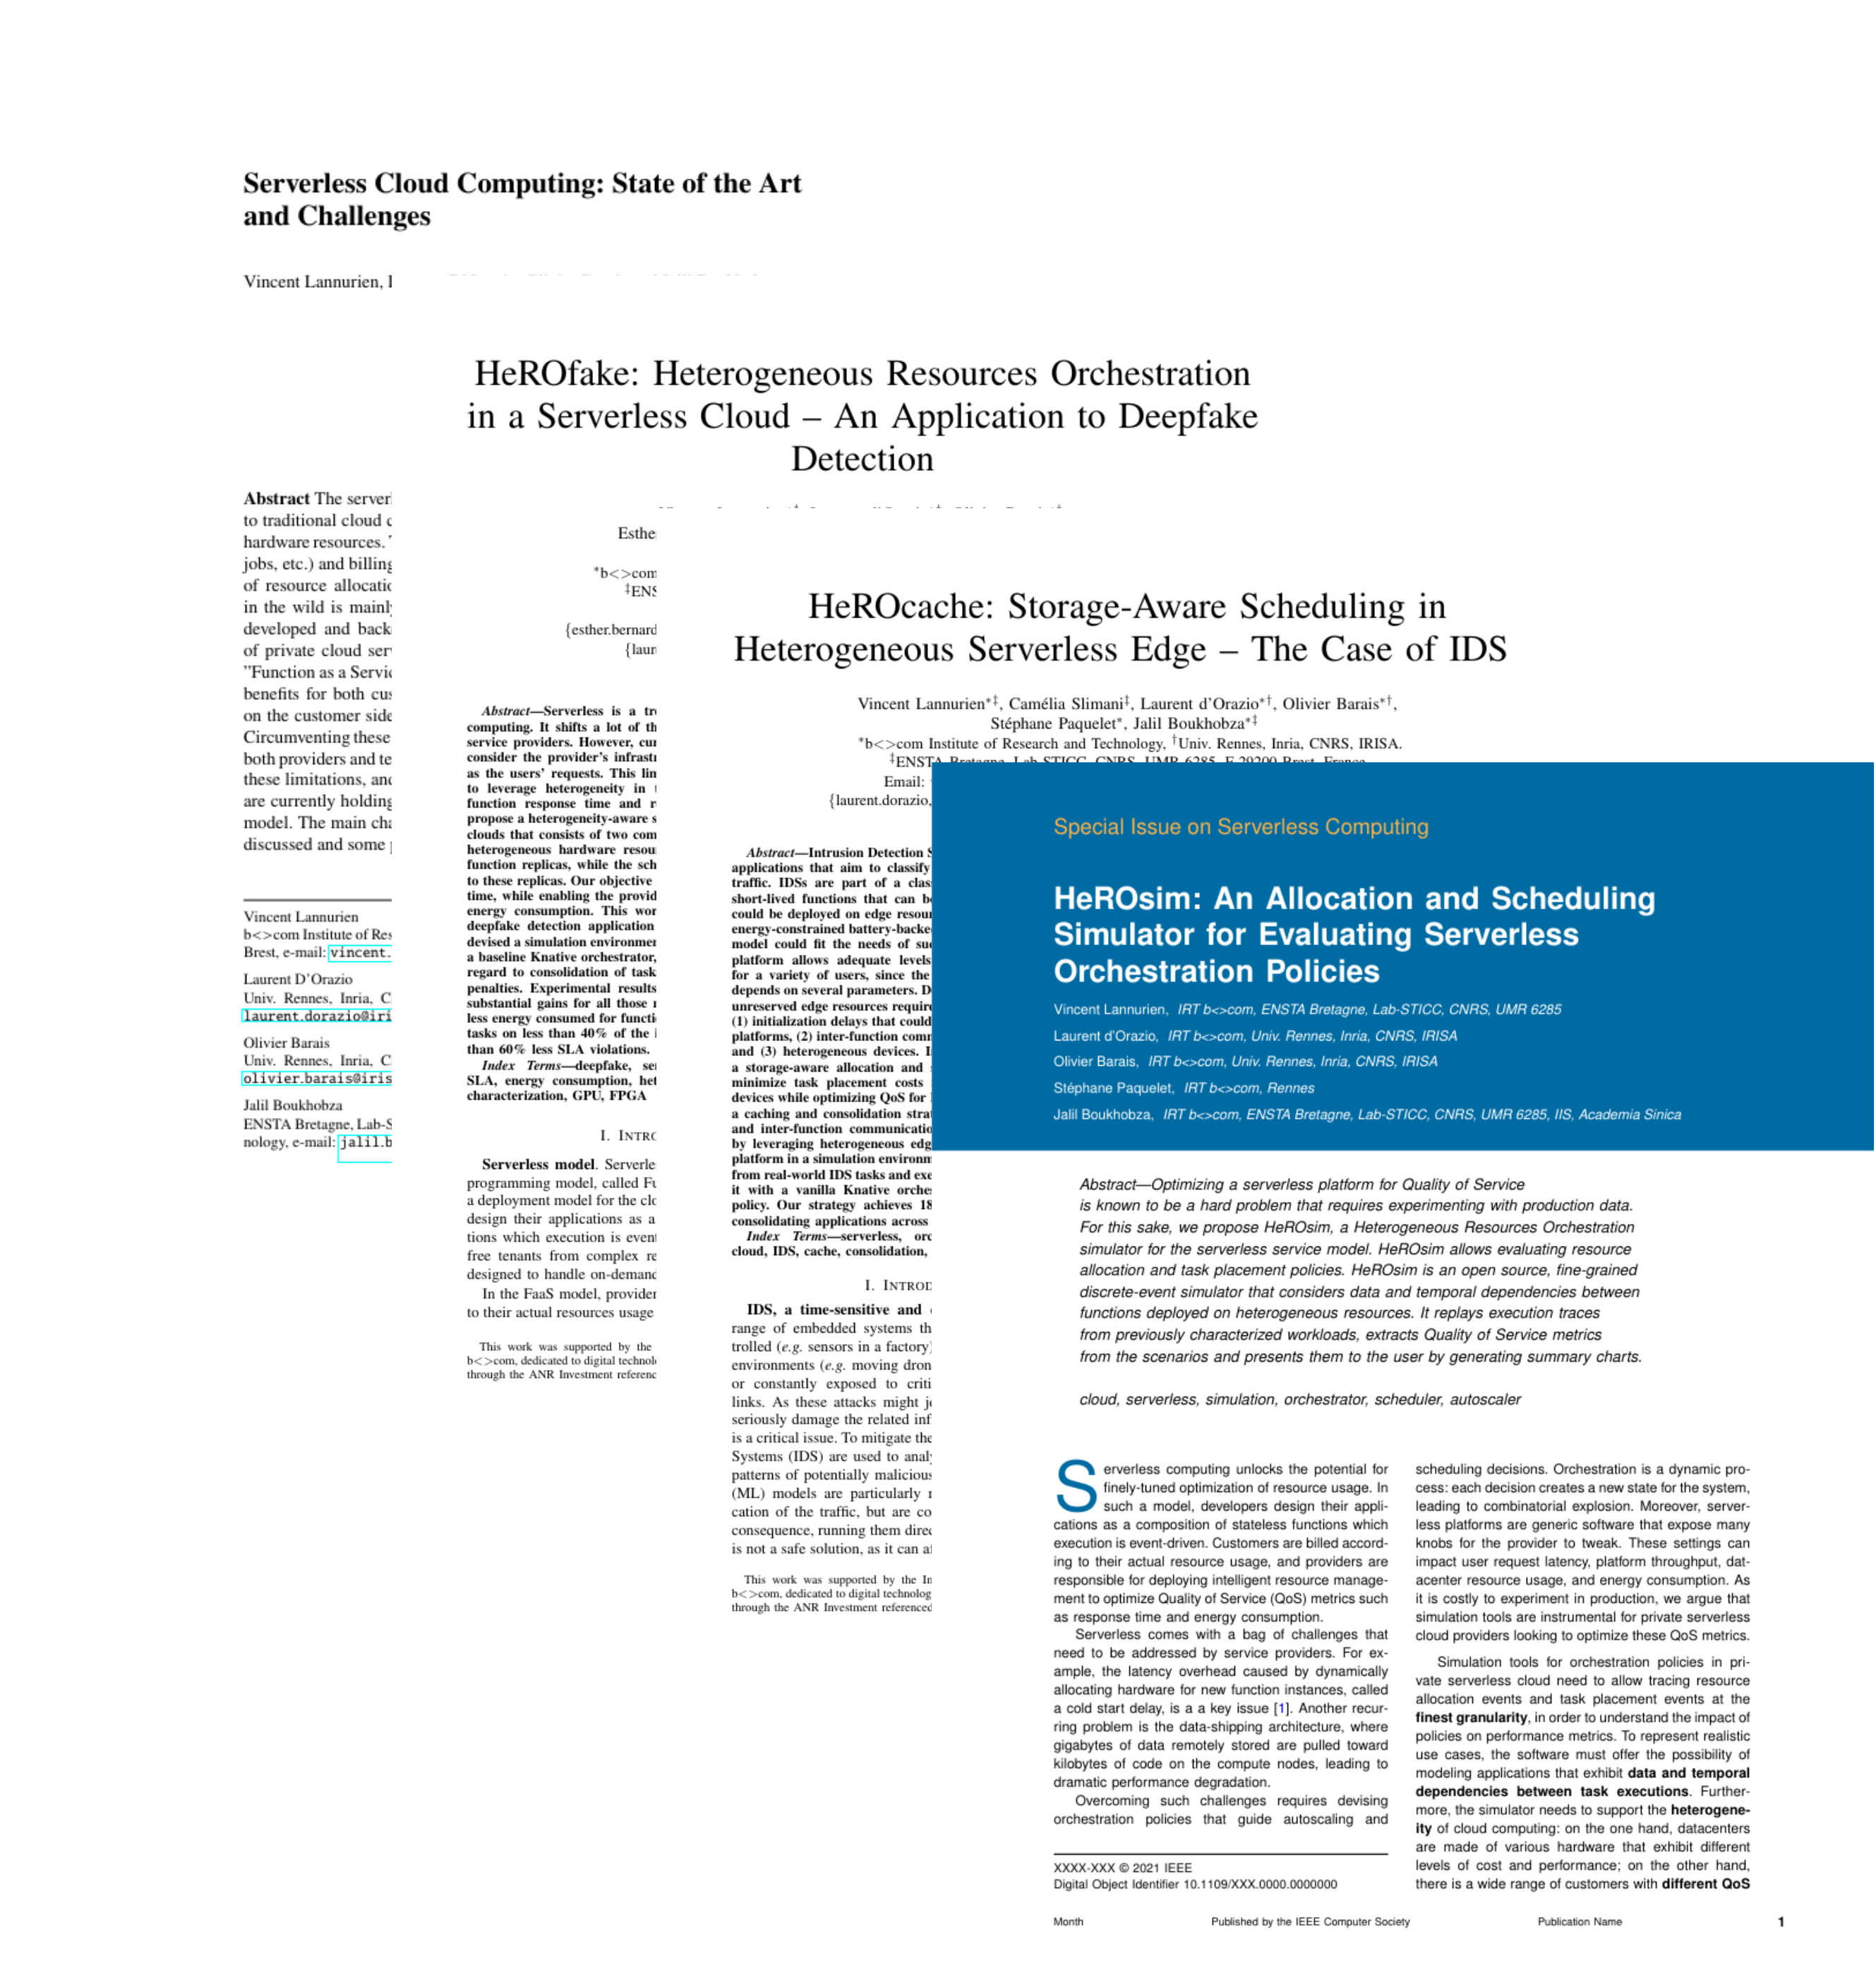
\includegraphics[width=0.9\columnwidth]{img/toc.png}
        \end{center}
    \end{columns}
\end{frame}
\end{framefont}

\section{Contexte}

\begin{frame}{\textit{Cloud computing} : une définition}
    \begin{columns}
        \column{0.45\textwidth}
        \begin{itemize}
            \item Définition donnée par le NIST~\footnote[frame]{\fullcite{mellNISTDefinitionCloud}} :
            \begin{itemize}
                \item Service \textbf{à la demande} ;
                \item \textbf{Accessible} par le réseau ;
                \item Ressources \textbf{partagées} ;
                \item \textbf{Élasticité} rapide ;
                \item Service \textbf{mesuré}.
            \end{itemize}
        \end{itemize}

        \begin{center}
            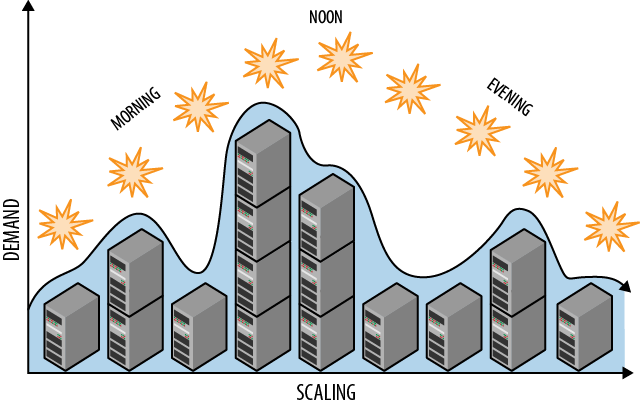
\includegraphics[width=0.8\columnwidth]{img/cloud-scaling.png}
        \end{center}

        \column{0.45\textwidth}
        \begin{center}
            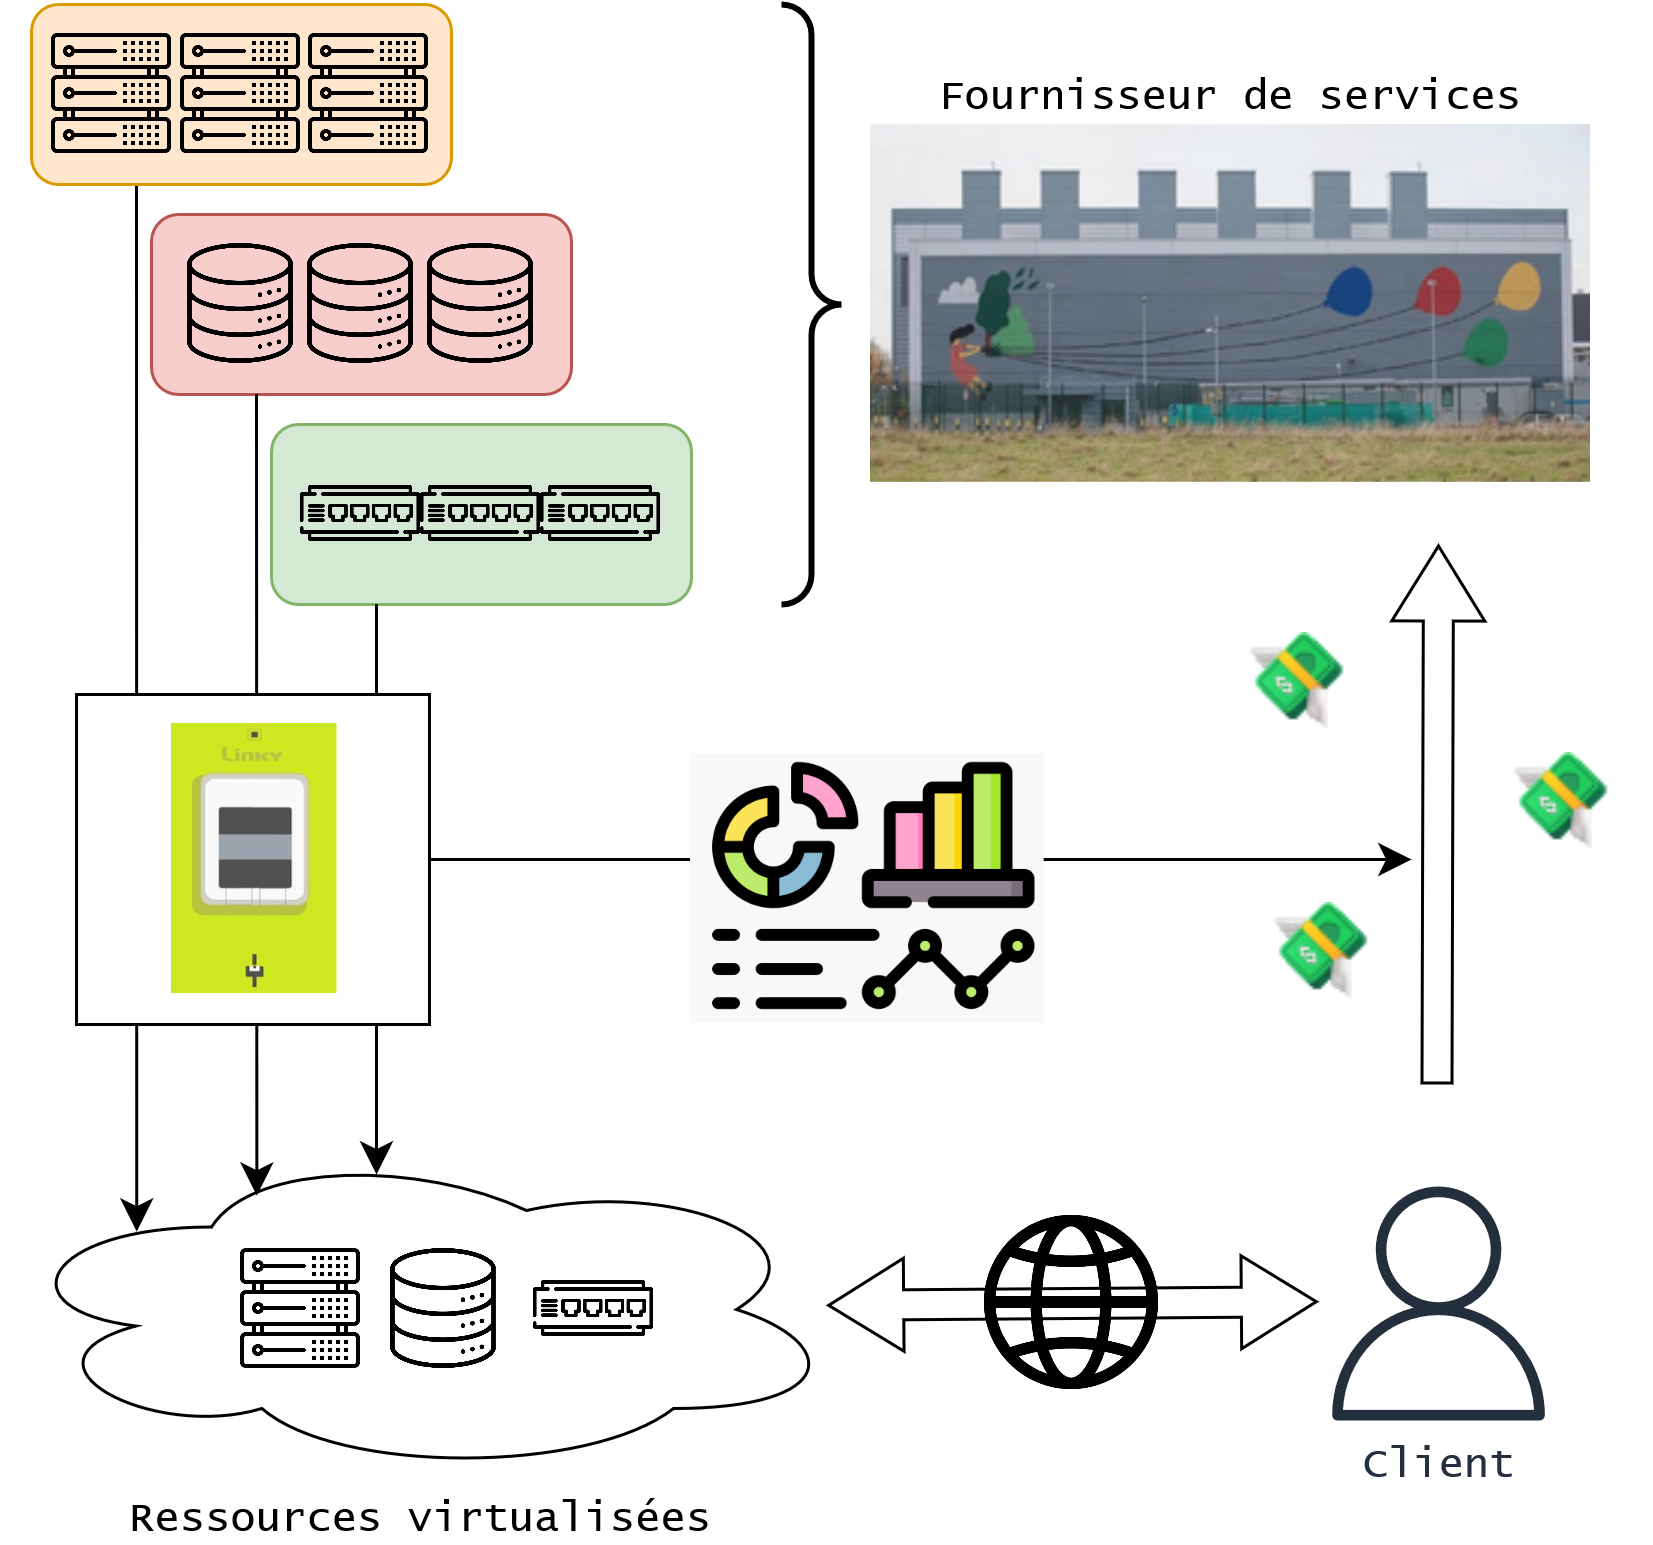
\includegraphics[width=\columnwidth]{img/cloud.png}
        \end{center}
    \end{columns}

    \addtocounter{footnote}{1}
    \footnotetext{\fullcite{wilder2012cloud}}
\end{frame}

\begin{frame}{Problématique : dimensionnement}
    \begin{columns}
        \column{0.5\textwidth}
        \begin{itemize}
            \item Dimensionnement aux pics
            \begin{itemize}
                \item \textit{Over provisioning}
            \end{itemize}
            \item Exigences de QoS
            \begin{itemize}
                \item \textit{Over committing}
            \end{itemize}
            \item Ressources dormantes
            \begin{itemize}
                \item \textit{Under utilization}
            \end{itemize}
        \end{itemize}

        \begin{center}
            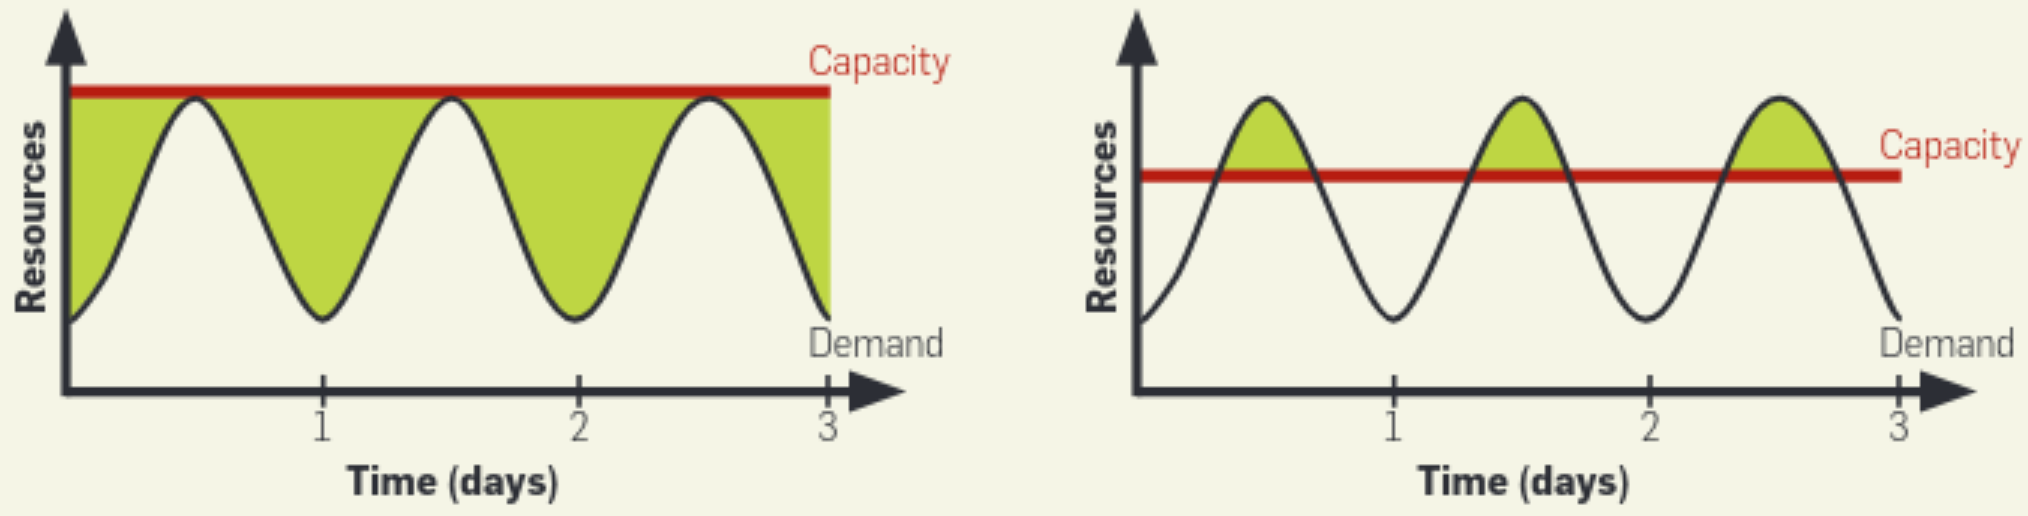
\includegraphics[width=\columnwidth]{img/dimensionnement-1.png}
        \end{center}

        \column{0.5\textwidth}
        \begin{center}
            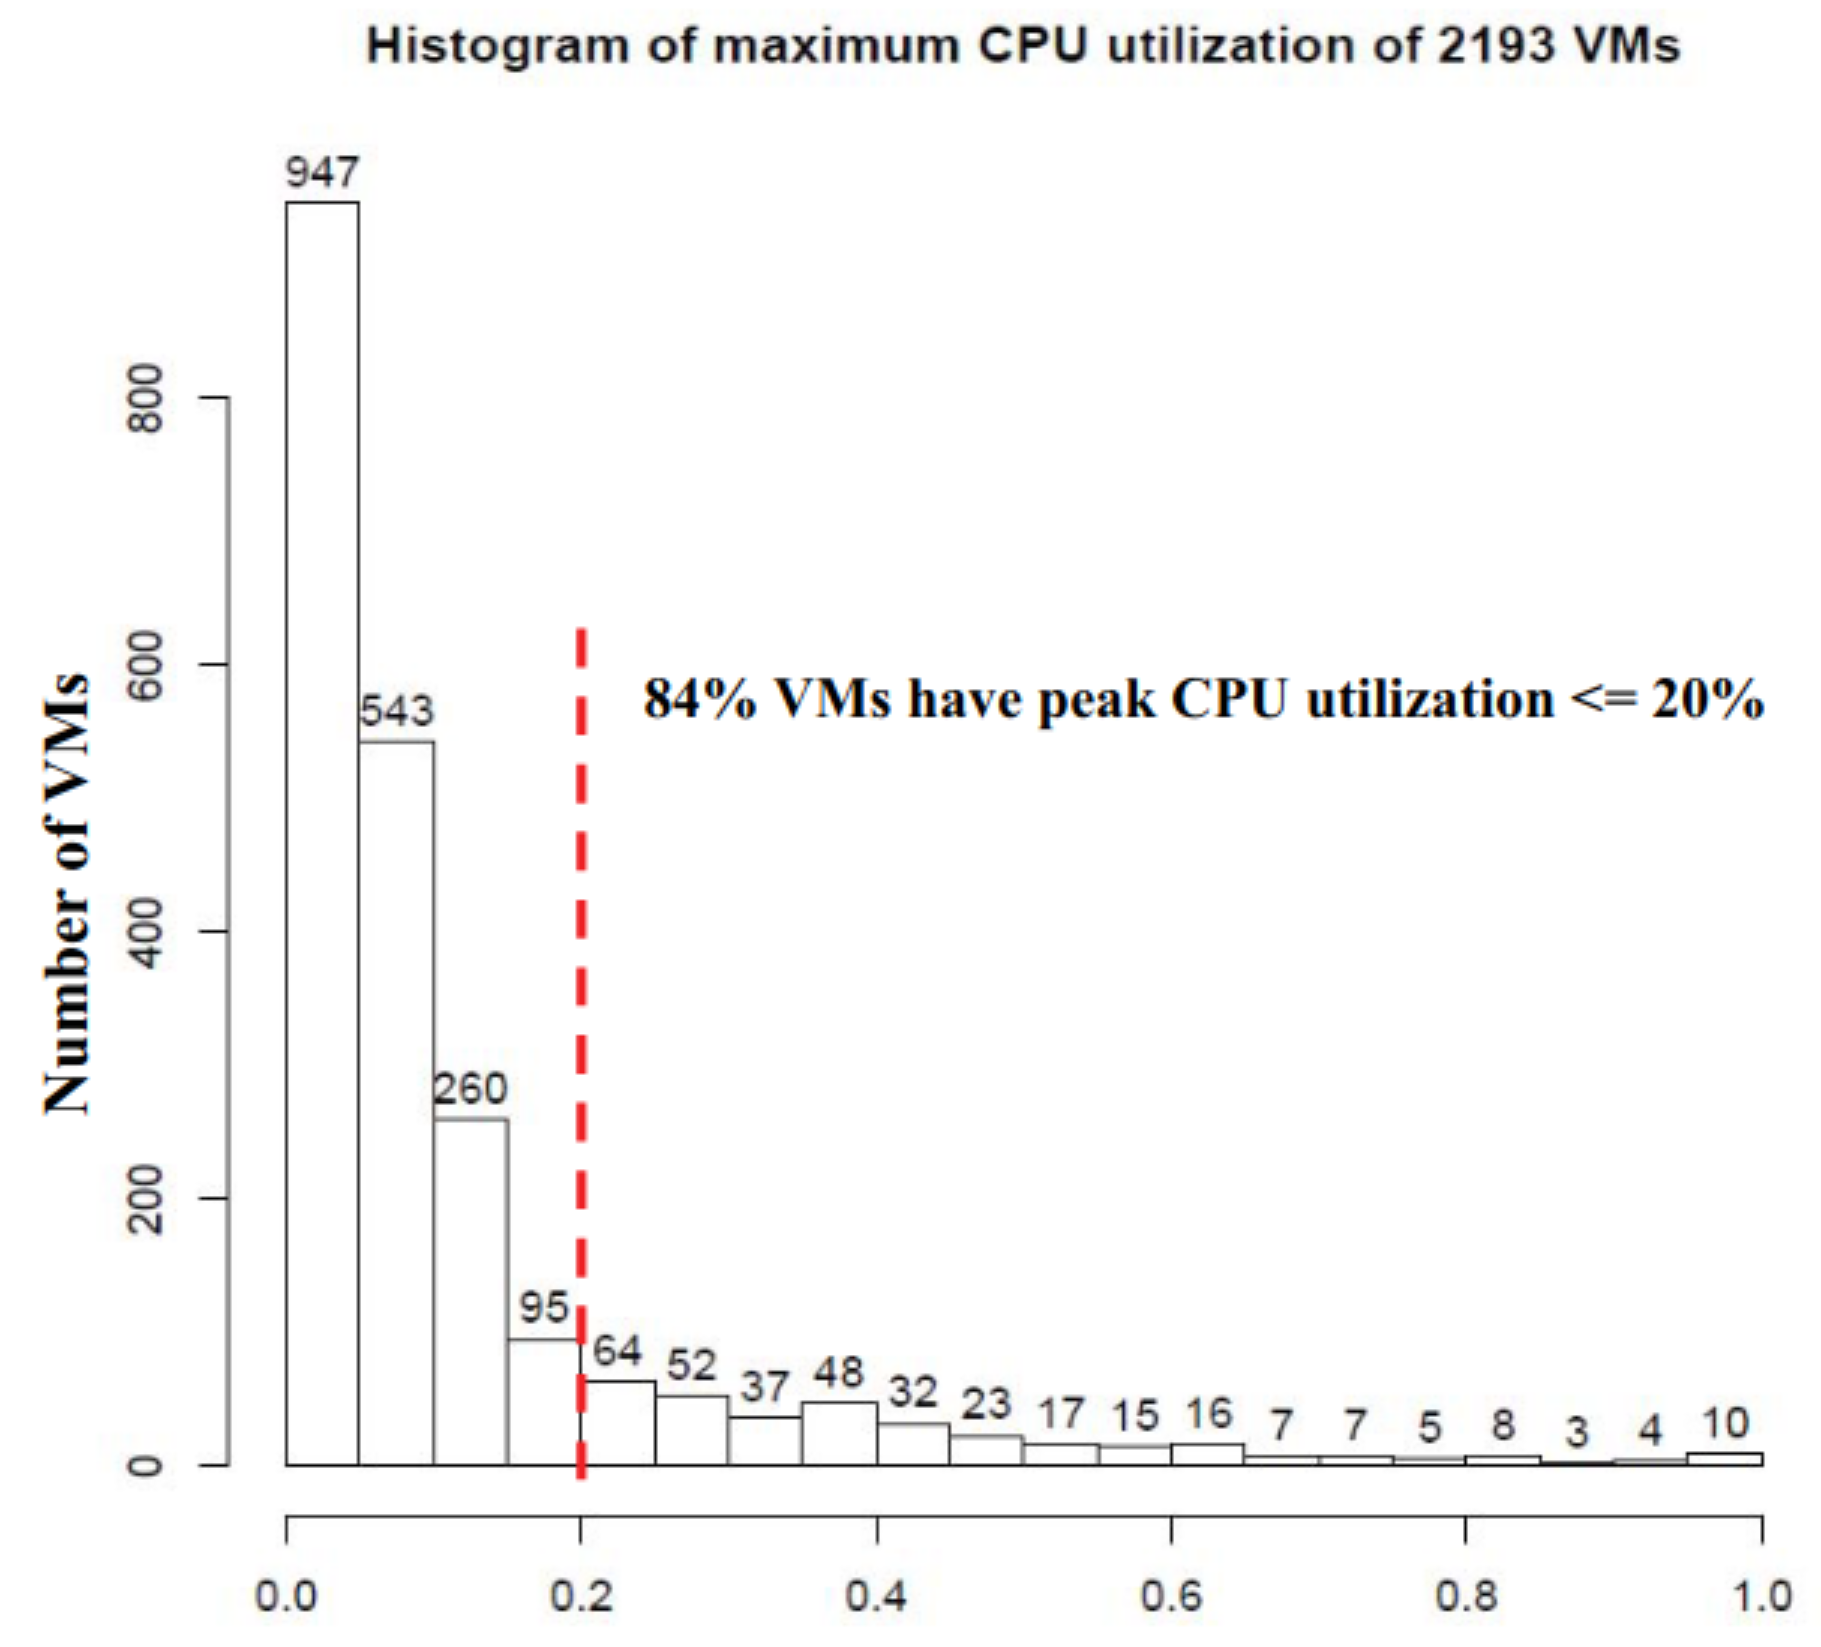
\includegraphics[width=0.8\columnwidth]{img/dimensionnement-2.png}
        \end{center}
    \end{columns}

    \addtocounter{footnote}{1}
    \footnotetext{\fullcite{armbrustViewCloudComputing2010}}
    \addtocounter{footnote}{1}
    \footnotetext{\fullcite{bitingoff_ghosh_2012}}
\end{frame}

\begin{frame}{Problématique : consommation d'énergie}
    \begin{columns}
        \column{0.6\textwidth}
        \resizebox{0.8\textwidth}{!}{\vbox{
            \begin{itemize}
                \item Énergie dans le cloud :
                \begin{itemize}
                    \item 2010 : $\sim$ 1,5\% de la consommation mondiale (273 TWh)~\footnote[frame]{\fullcite{masanetRecalibratingGlobalData2020}} ;
                    \item $\sim$ 4\% de la demande d'énergie en Europe~\footnote[frame]{\fullcite{Electricity2024Analysis2024}};
                \end{itemize}
                \item Utilisation des ressources :
                \begin{itemize}
                    \item Centres de données américains : 10 à 30\% des serveurs \textbf{inactifs}~\footnote[frame]{\fullcite{shehabiUnitedStatesData2016a}} ;
                    \item Taux d'utilisation des ressources cloud : \textless 15\%~\footnote[frame]{\fullcite{vasanWorthTheirWatts2010}} ;
                    \item Serveurs consomment 80\% de leur énergie à 20\% d'utilisation réelle~\footnote[frame]{\fullcite{pedramEnergyEfficientDatacenters2012}}.
                \end{itemize}
                \item Secteur en forte croissance : 15 à 20\% par an d'ici à 2030~\footnote[frame]{\fullcite{WorldwideSpendingPublic}} (tolérance aux pannes, prédiction de la demande future)
            \end{itemize}
        }}

        \column{0.4\textwidth}
        \begin{center}
            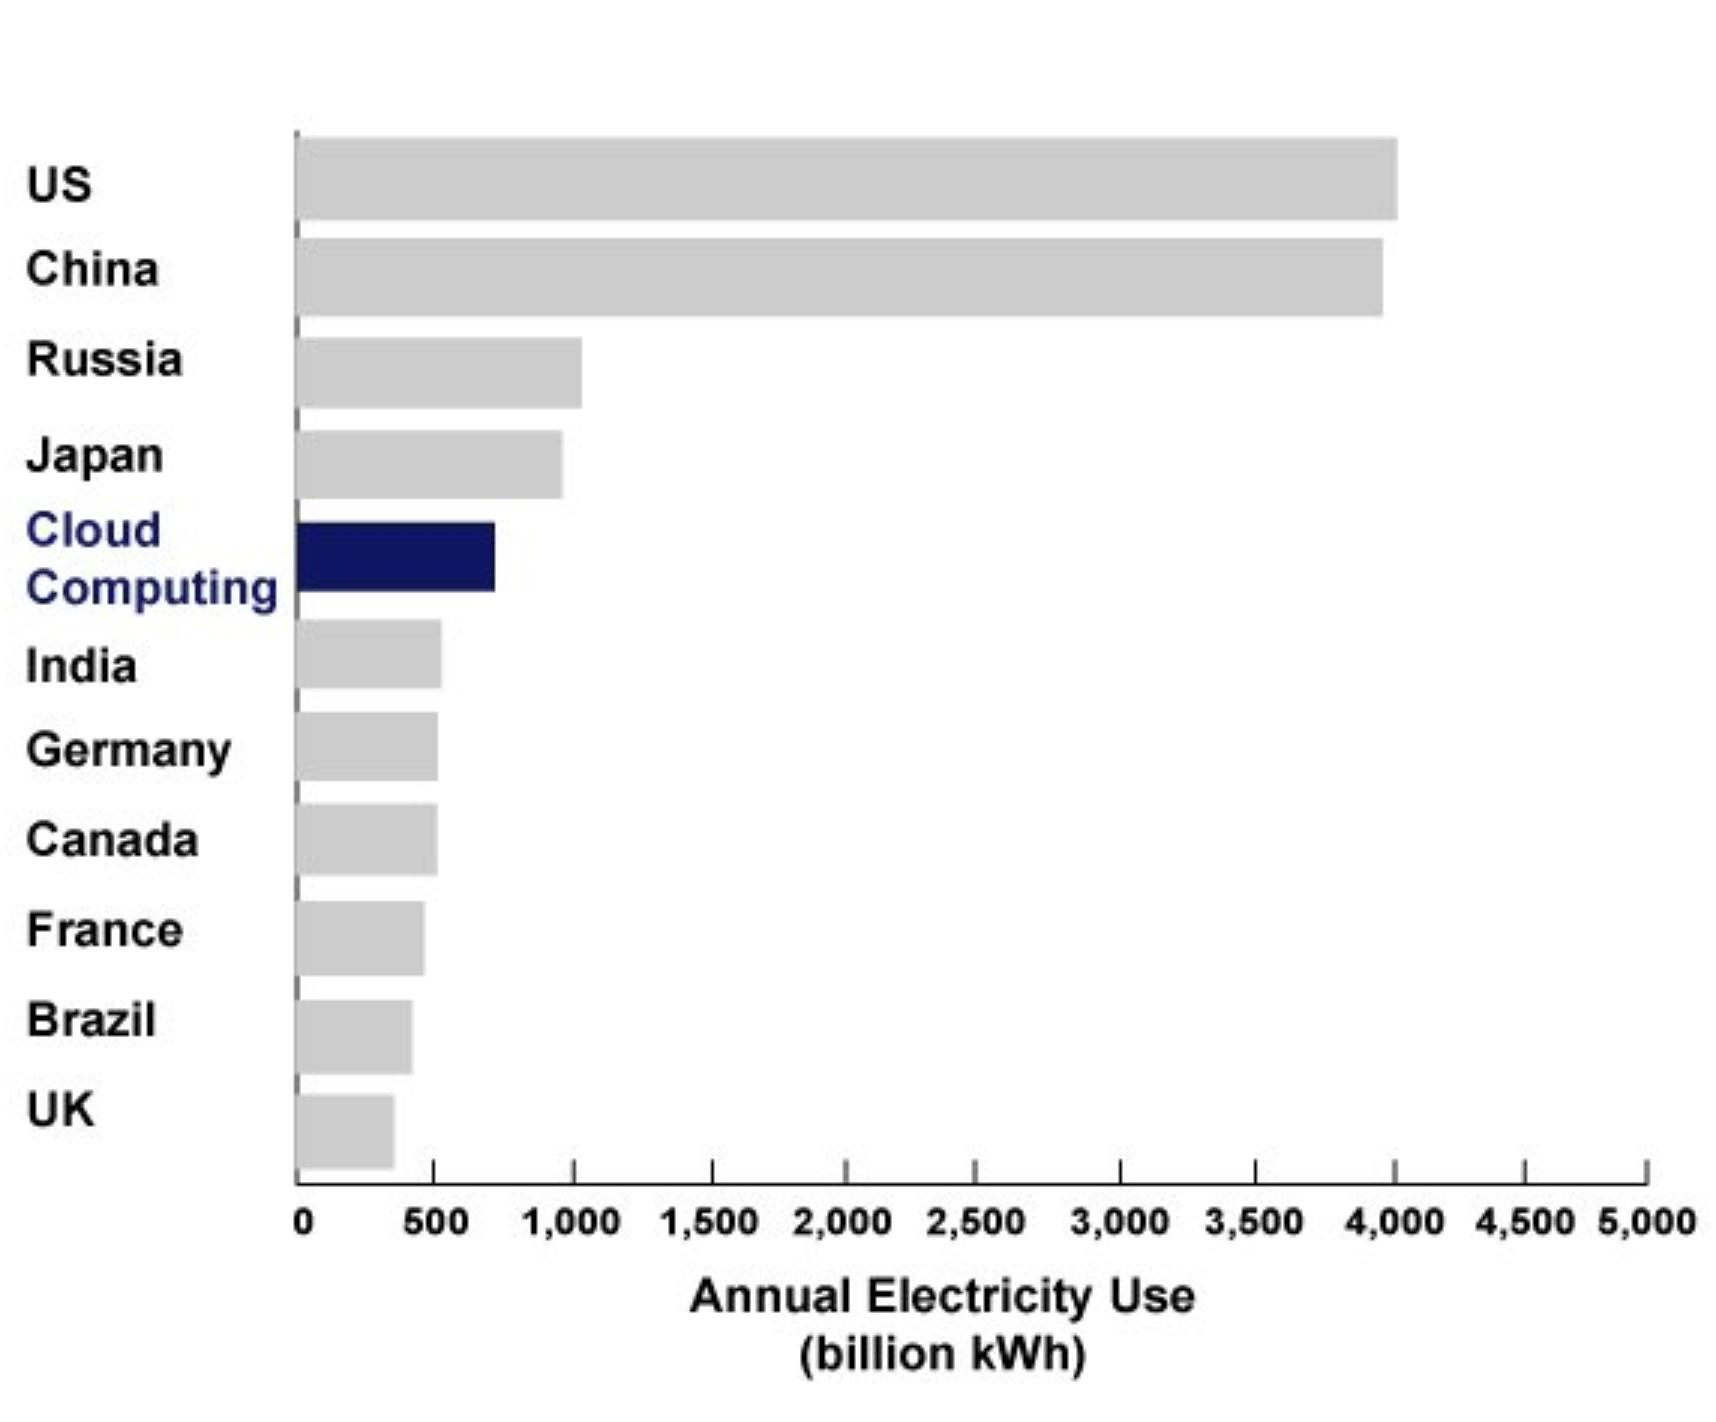
\includegraphics[width=\columnwidth]{img/energy-1.png}
        \end{center}
    \end{columns}

    \addtocounter{footnote}{1}
    \footnotetext{\fullcite{Numerique40Budget2021}}
\end{frame}

\begin{frame}{\textit{Serverless computing} : une définition}
    \begin{columns}
        \column{0.6\textwidth}
        \begin{itemize}
            \item Une nouvelle abstraction pour le cloud :
            \begin{itemize}
                \item Unité d'allocation : \textbf{temps} plutôt que \textbf{ressource} ;
                \item Granularité fine : déploiement de \textbf{fonctions} ;
                \item Déplacement de la responsabilité : de l'utilisateur vers le fournisseur de services.
            \end{itemize}
        \end{itemize}

        \begin{center}
            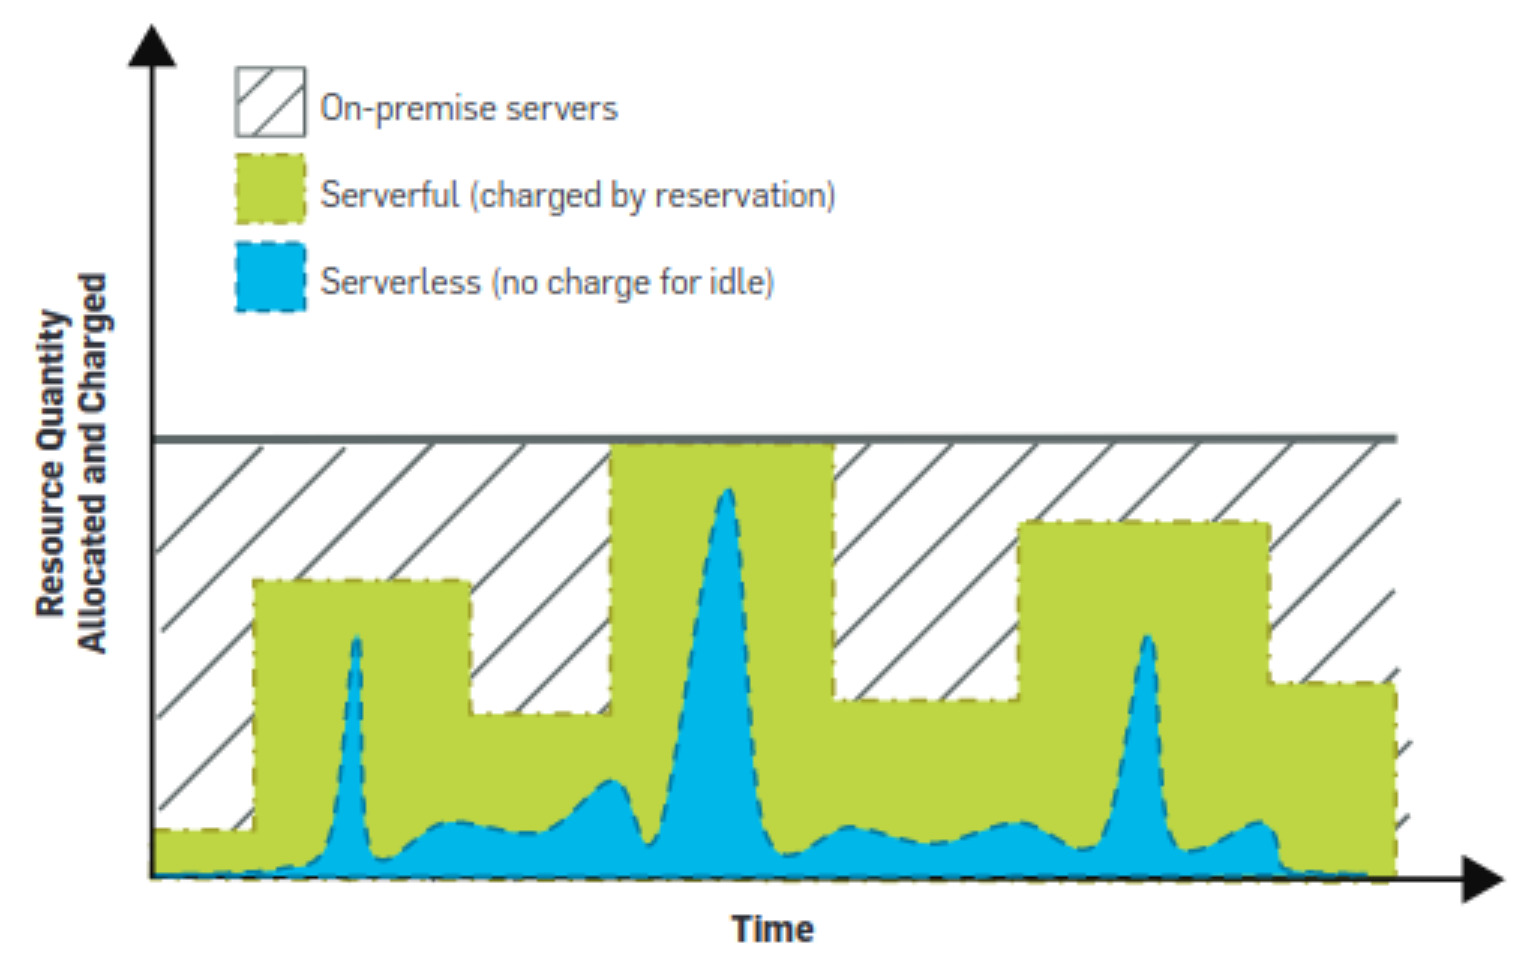
\includegraphics[width=0.8\columnwidth]{img/serverless.png}
        \end{center}

        \column{0.35\textwidth}
        \begin{center}
            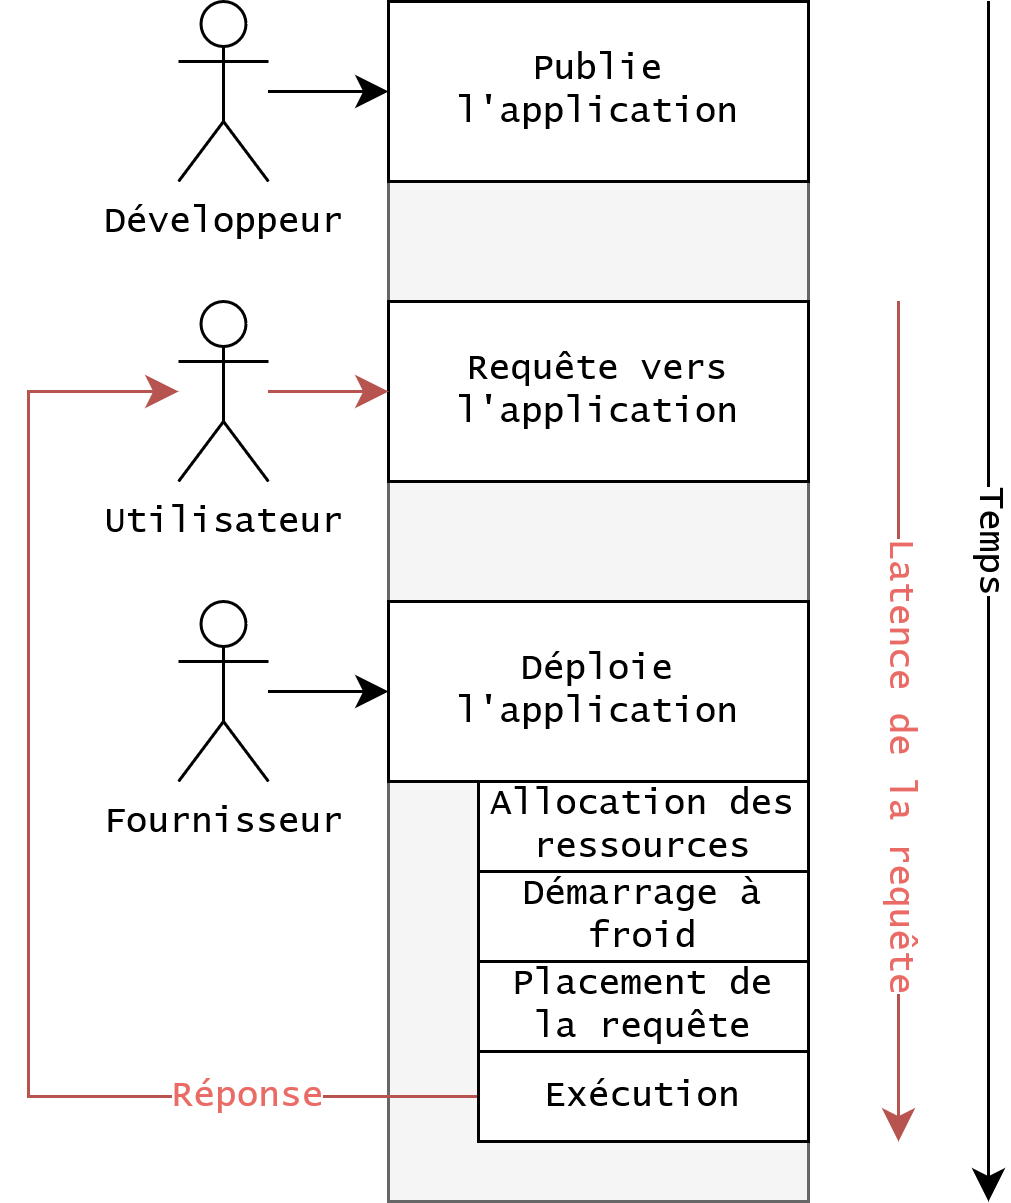
\includegraphics[width=0.9\columnwidth]{img/serverless-timeline.png}
        \end{center}
    \end{columns}

    \footnotetext{\fullcite{SchleierSmith2021WhatSC}}
\end{frame}

\note[enumerate]{
    \item Ce qui est masqué par la courbe bleue, c'est le coût en latence des allocations dynamiques : le démarrage à froid des fonctions
}

\begin{frame}{\textit{Cloud computing} : une affaire de compromis}
    \begin{columns}
        \column{0.5\textwidth}
        \begin{center}
            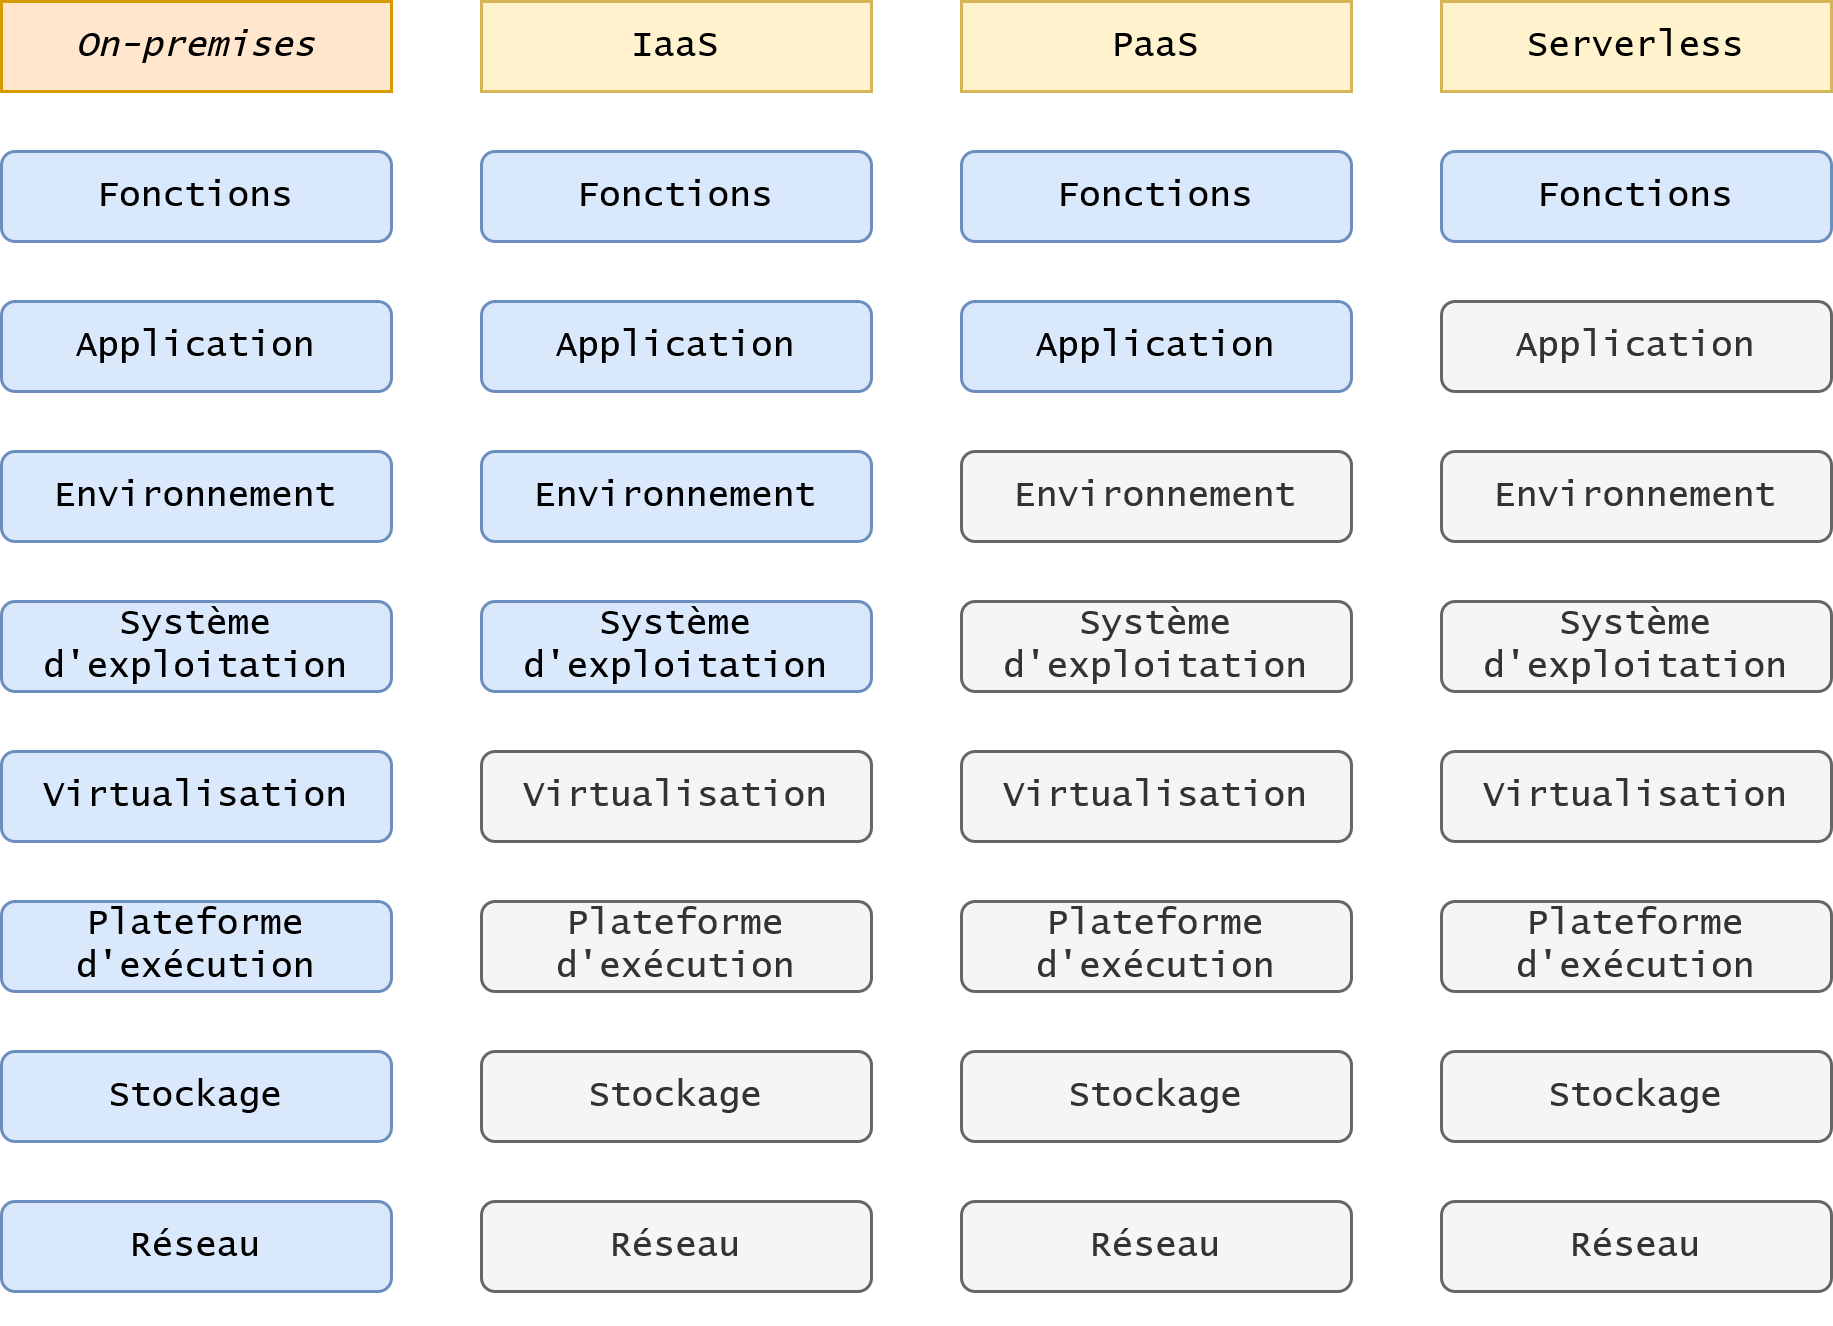
\includegraphics[width=\columnwidth]{img/service-models.png}
        \end{center}

        \column{0.5\textwidth}
        \begin{center}
            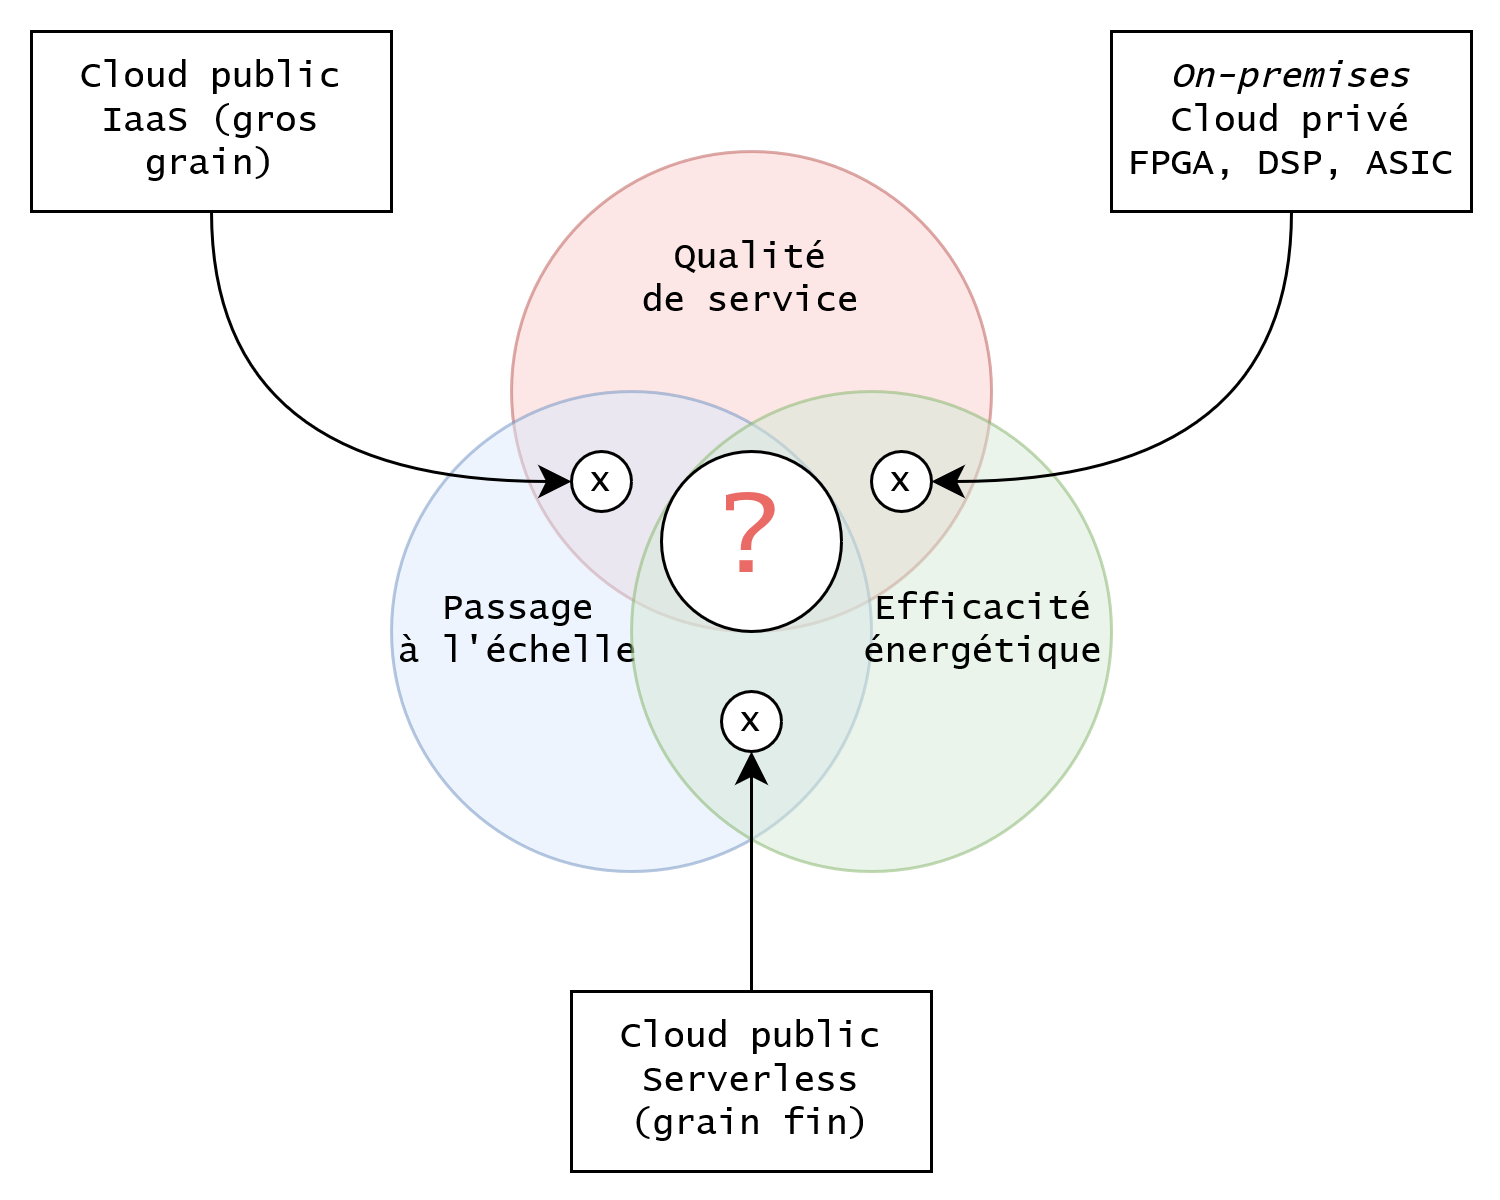
\includegraphics[width=\columnwidth]{img/heterogeneity.png}
        \end{center}
    \end{columns}
\end{frame}

\note[enumerate]{
    \item Modèle de service dans le cloud public : \textit{Function as a Service}
    \item AWS Lambda, Google Cloud Functions, Azure Functions...
}

\begin{frame}{\textit{Serverless computing} : une définition}
    \begin{table}[]
        \centering
        \resizebox{0.9\textwidth}{!}{
            \begin{tabularx}{\textwidth}{ZZZ}
                \toprule
                \addlinespace[0.5em]
                \textbf{Caractéristique} & \textbf{Serverful} & \textbf{Serverless} \\
                \addlinespace[0.5em]
                \midrule
                \addlinespace[0.5em]
                \textbf{Architecture logicielle} & Pas de contrainte & Découpage en fonctions sans état \\
                \textbf{Provisionnement} & En fonction de l'offre & Géré par le fournisseur \\
                \addlinespace[0.5em]
                \textbf{Mise à l'échelle} & \textit{Capacity planning} & Dimensionnement automatique \\
                \addlinespace[0.5em]
                \textbf{Disponibilité} & Dépend des ressources réservées & Nombreuses instances réparties \\
                \addlinespace[0.5em]
                \textbf{Tolérance aux fautes} & Dépend de la stratégie de l'utilisateur & Garantie par le fournisseur \\
                \addlinespace[0.5em]
                \textbf{Concurrence} & Dépend des ressources réservées & Virtuellement infinie \\
                \addlinespace[0.5em]
                \textbf{Mesure de l'utilisation} & Ressources provisionnées & Ressources utilisées \\
                \addlinespace[0.5em]
                \bottomrule
            \end{tabularx}
        }
    \end{table}

    \addtocounter{footnote}{1}
    \footnotetext{\fullcite{Lannurien2023}}
\end{frame}

\section{État de l'art}

\begin{frame}[t]{\textit{Serverless computing} : plateforme considérée}
    \begin{center}
        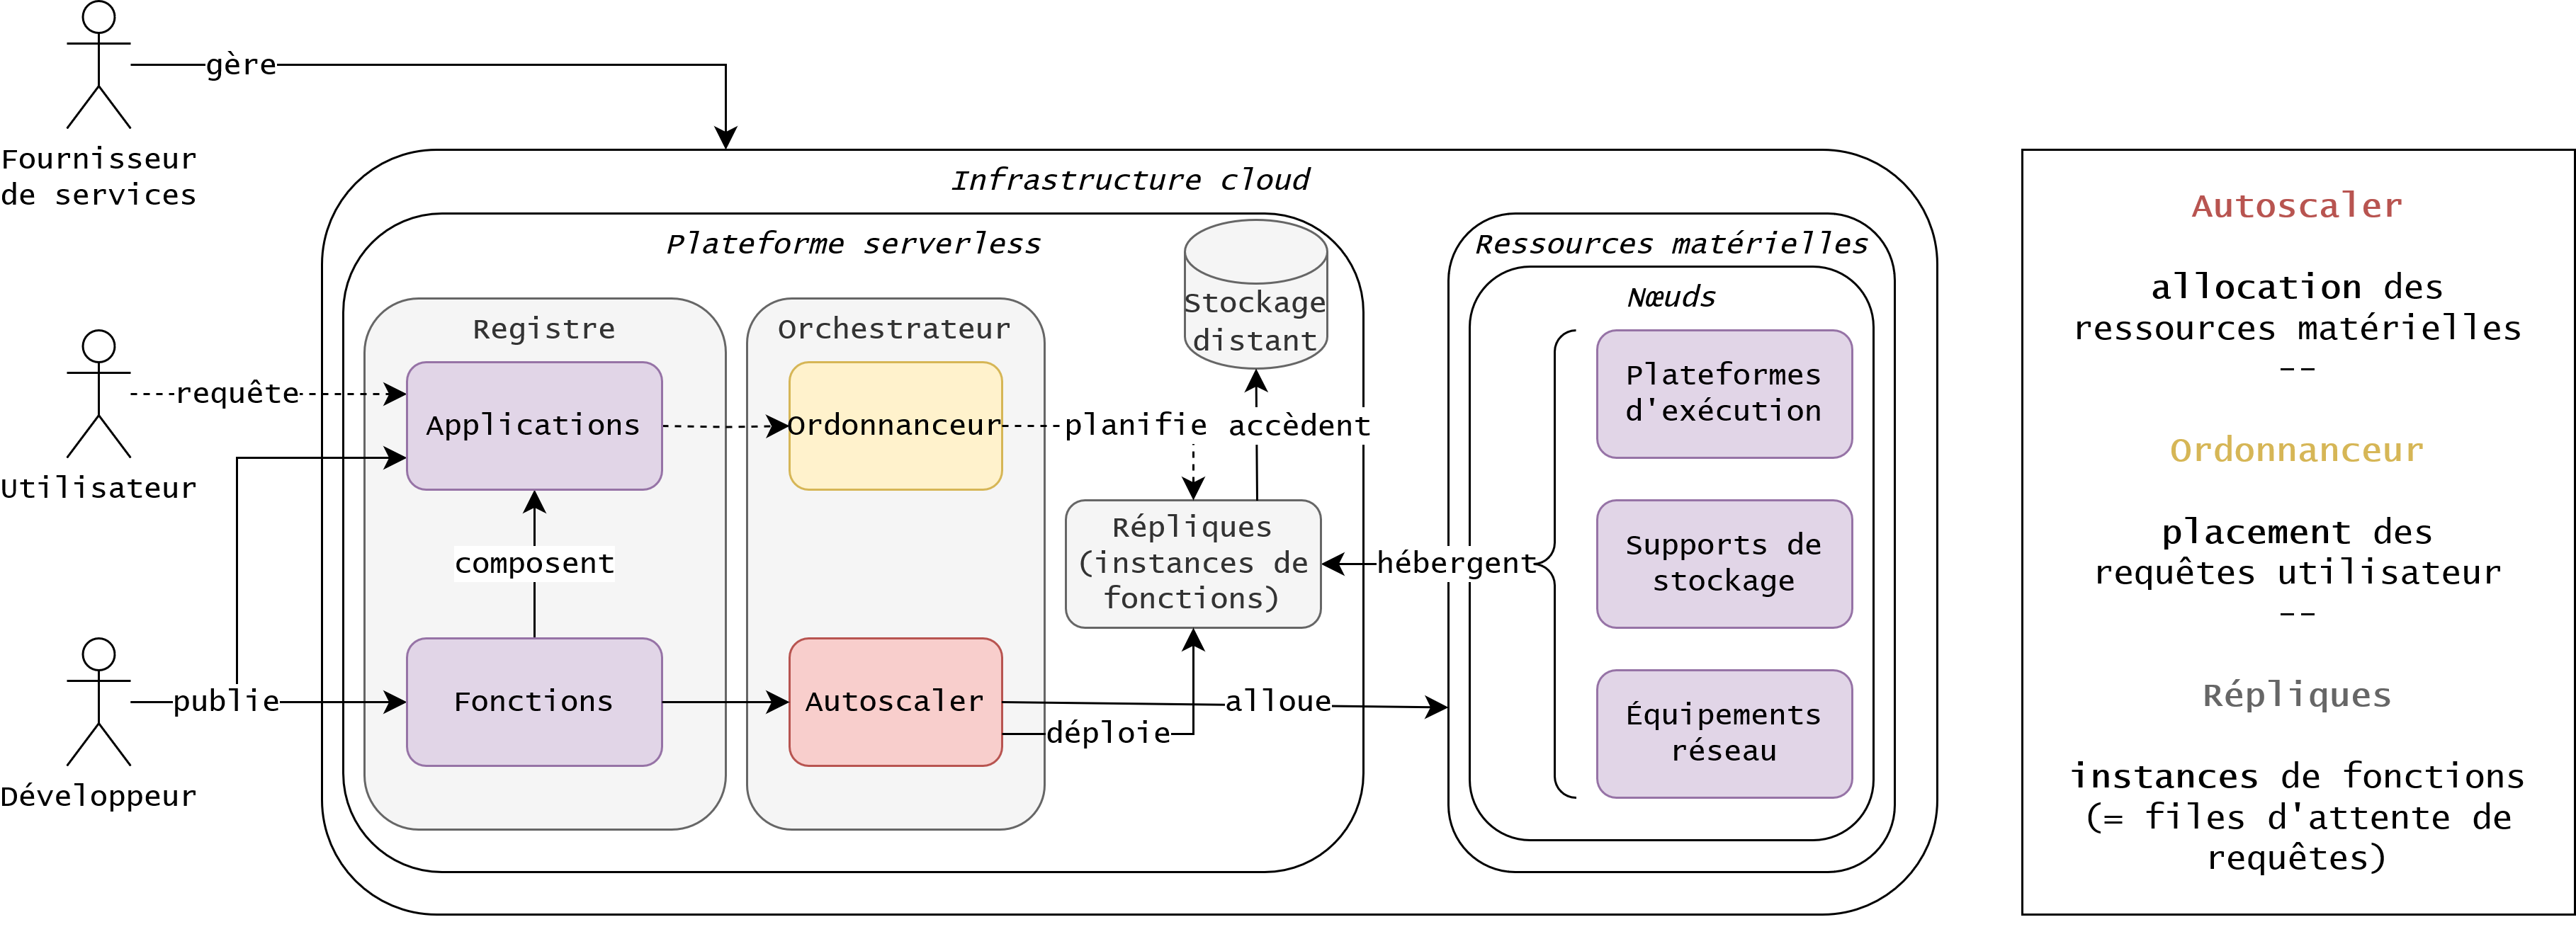
\includegraphics[width=\columnwidth]{img/plateforme-serverless.png}
    \end{center}

    \addtocounter{footnote}{1}
    \footnotetext{Google Knative -- \href{https://knative.dev}{https://knative.dev}}
    \addtocounter{footnote}{1}
    \footnotetext{Apache OpenWhisk -- \href{https://openwhisk.apache.org}{https://openwhisk.apache.org}}
\end{frame}

\begin{frame}[t]{\textit{Serverless computing} : défis}
    \begin{center}
        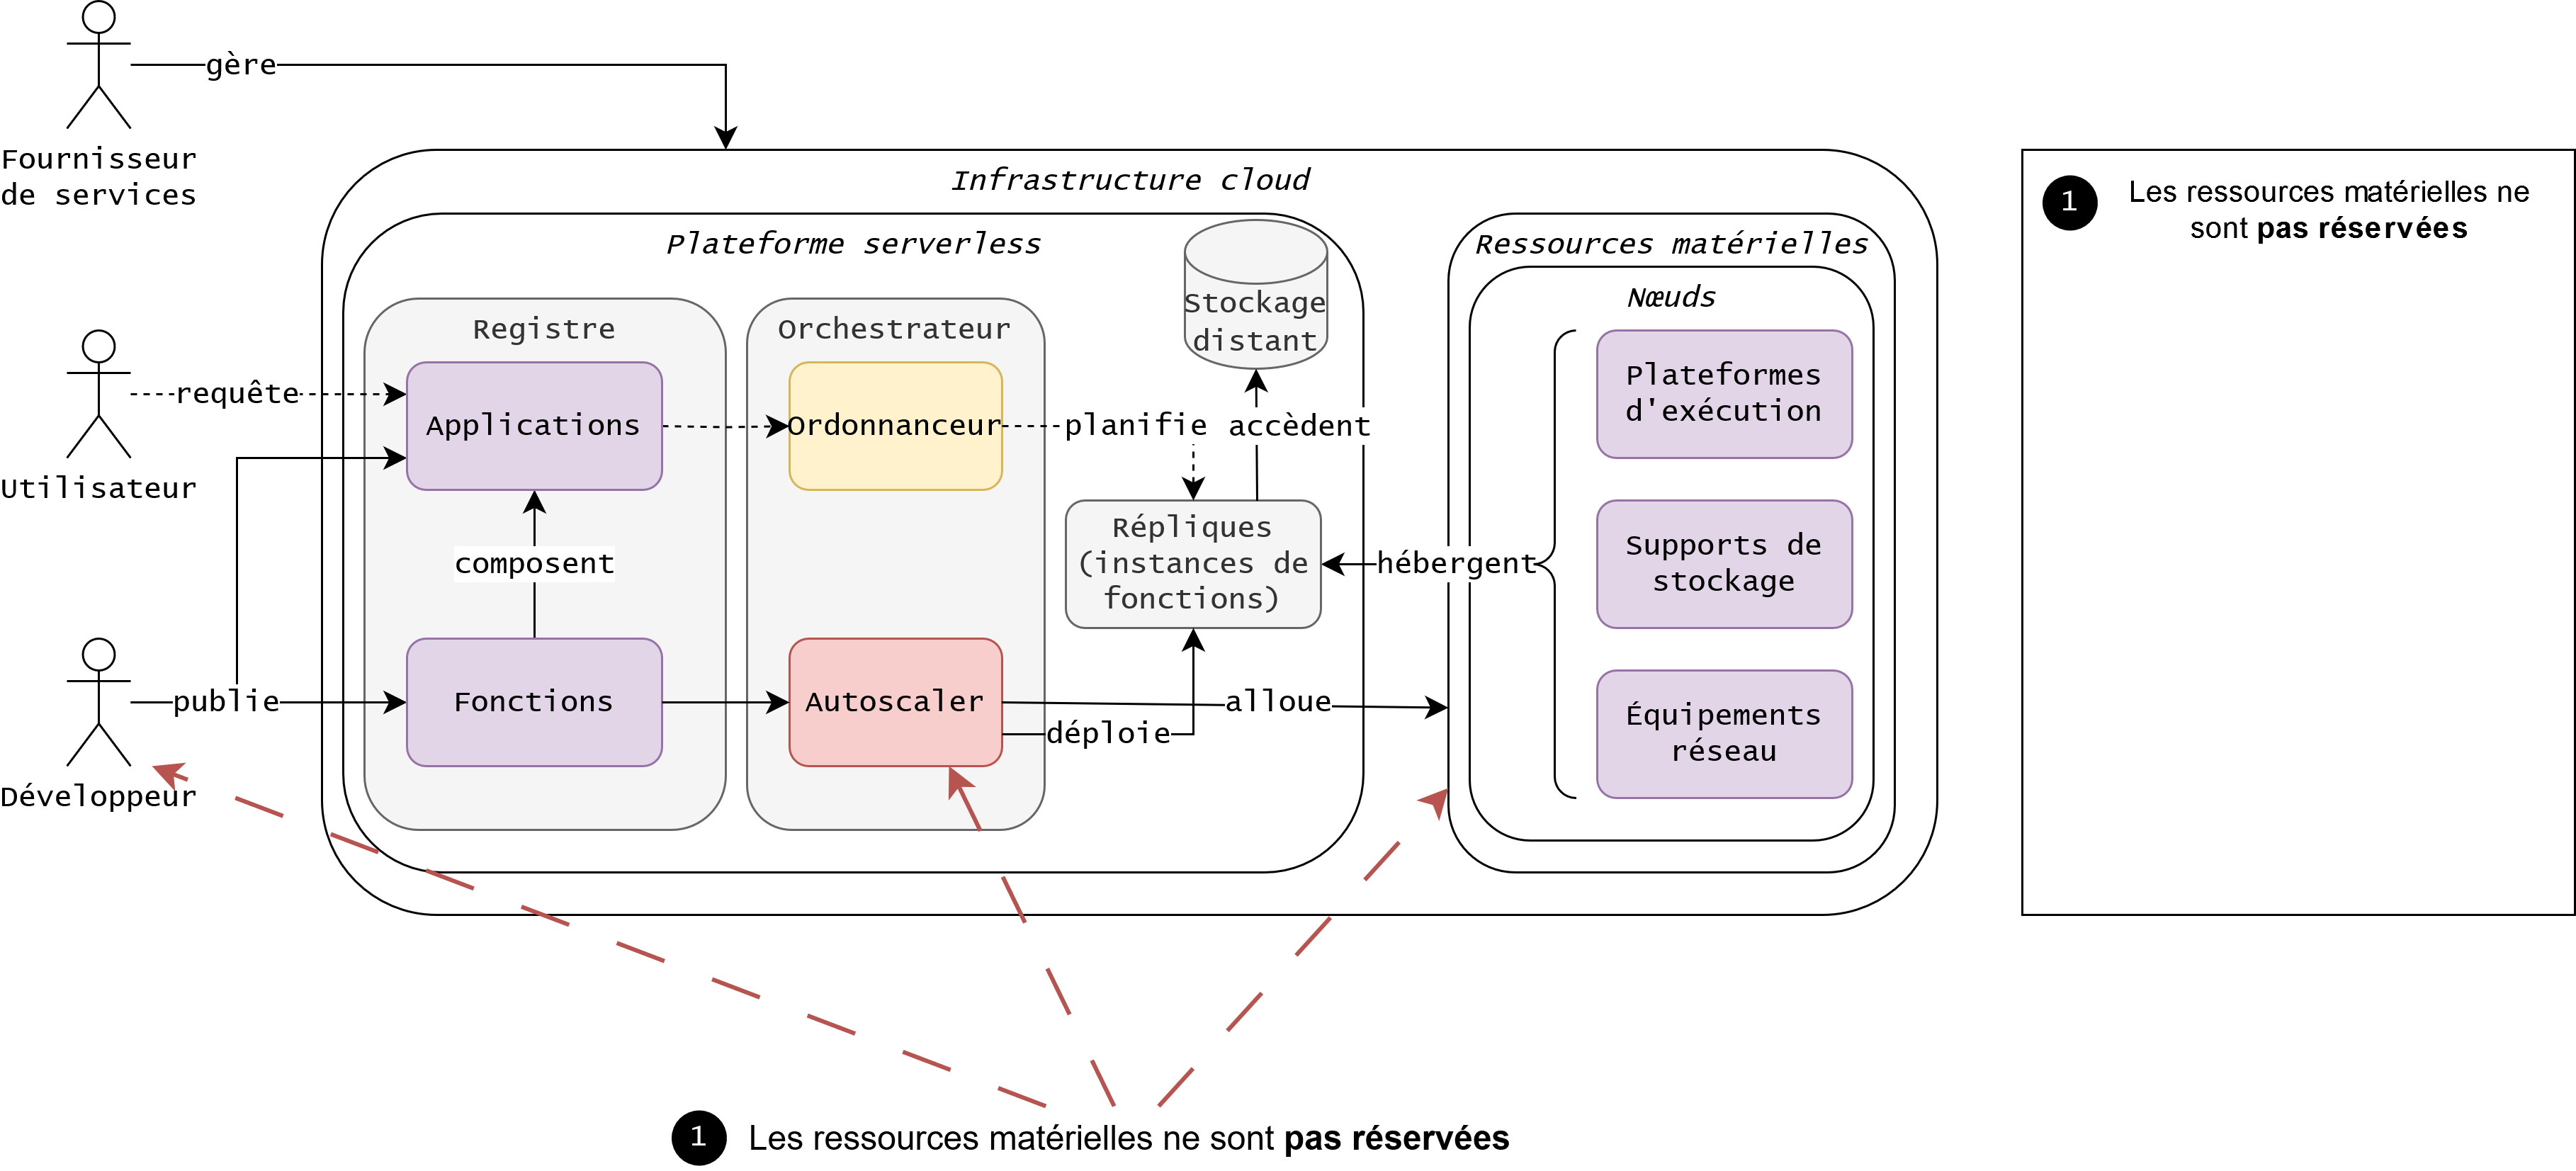
\includegraphics[width=\columnwidth]{img/sota-1.png}
    \end{center}

    \addtocounter{footnote}{1}
    \footnotetext{\fullcite{SchleierSmith2021WhatSC}}
\end{frame}

\note[enumerate]{
    \item \textbf{Allocation} dynamique (en fonction des variations de charge)
    \item \textbf{Placement} dynamique (des requêtes sur les ressources)
}

\begin{frame}[t,noframenumbering]{\textit{Serverless computing} : défis}
    \begin{center}
        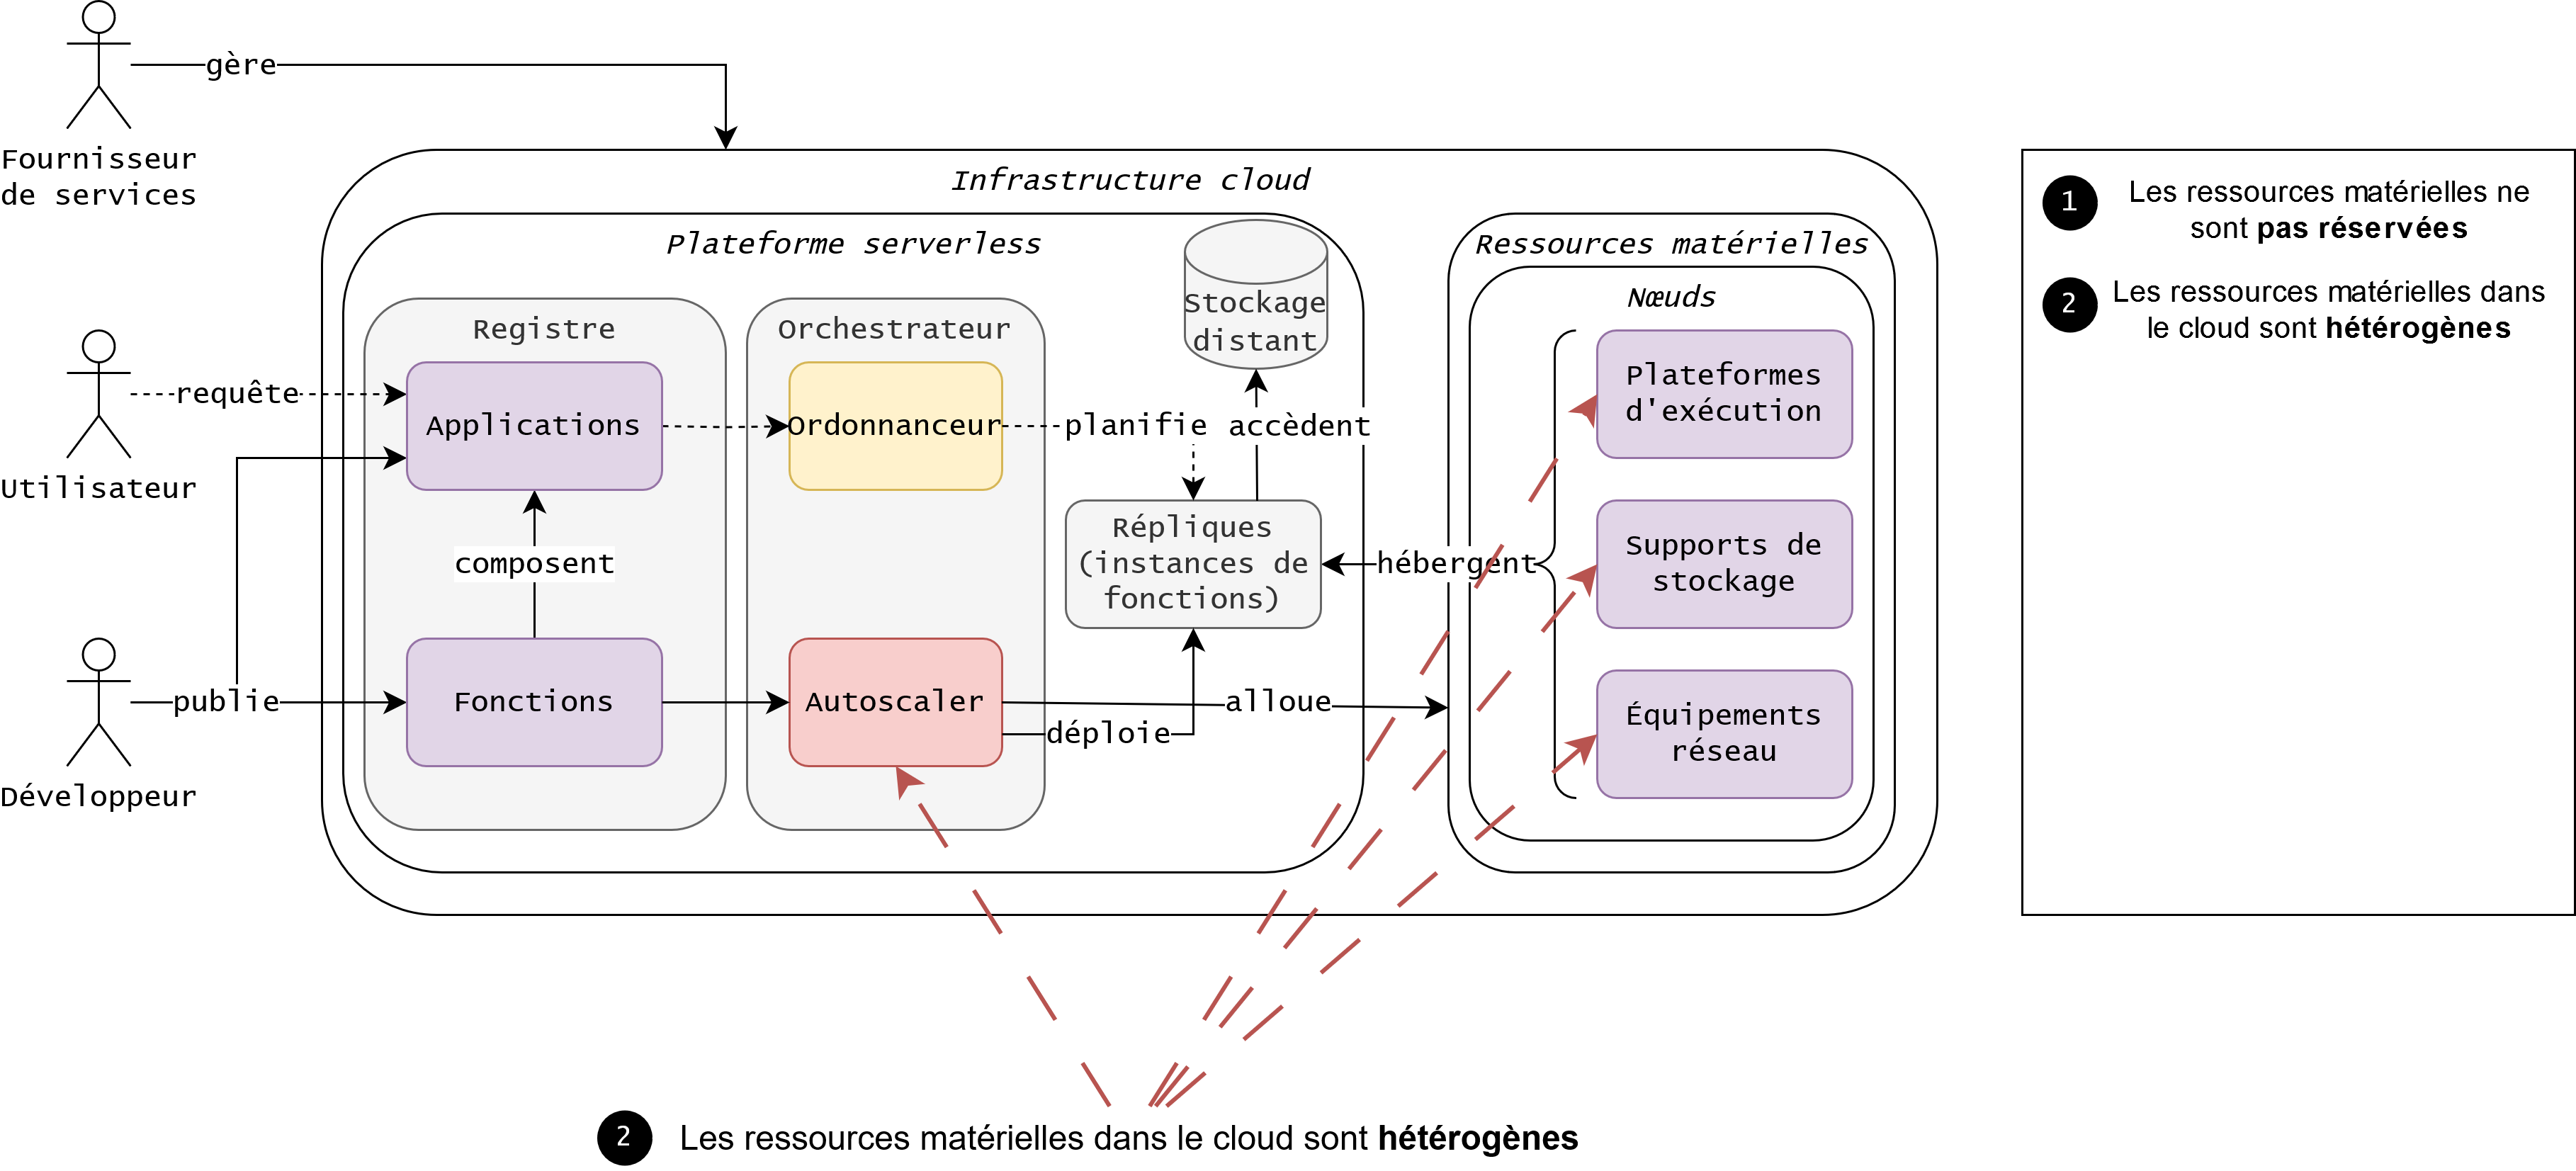
\includegraphics[width=\columnwidth]{img/sota-2.png}
    \end{center}

    \addtocounter{footnote}{1}
    \footnotetext{\fullcite{hortaXartrekRuntimeExecution2021}}
\end{frame}

\note[enumerate]{
    \item Différents niveaux de \textbf{performance}
    \item Différents profils de \textbf{coût}
}

\begin{frame}[t,noframenumbering]{\textit{Serverless computing} : défis}
    \begin{center}
        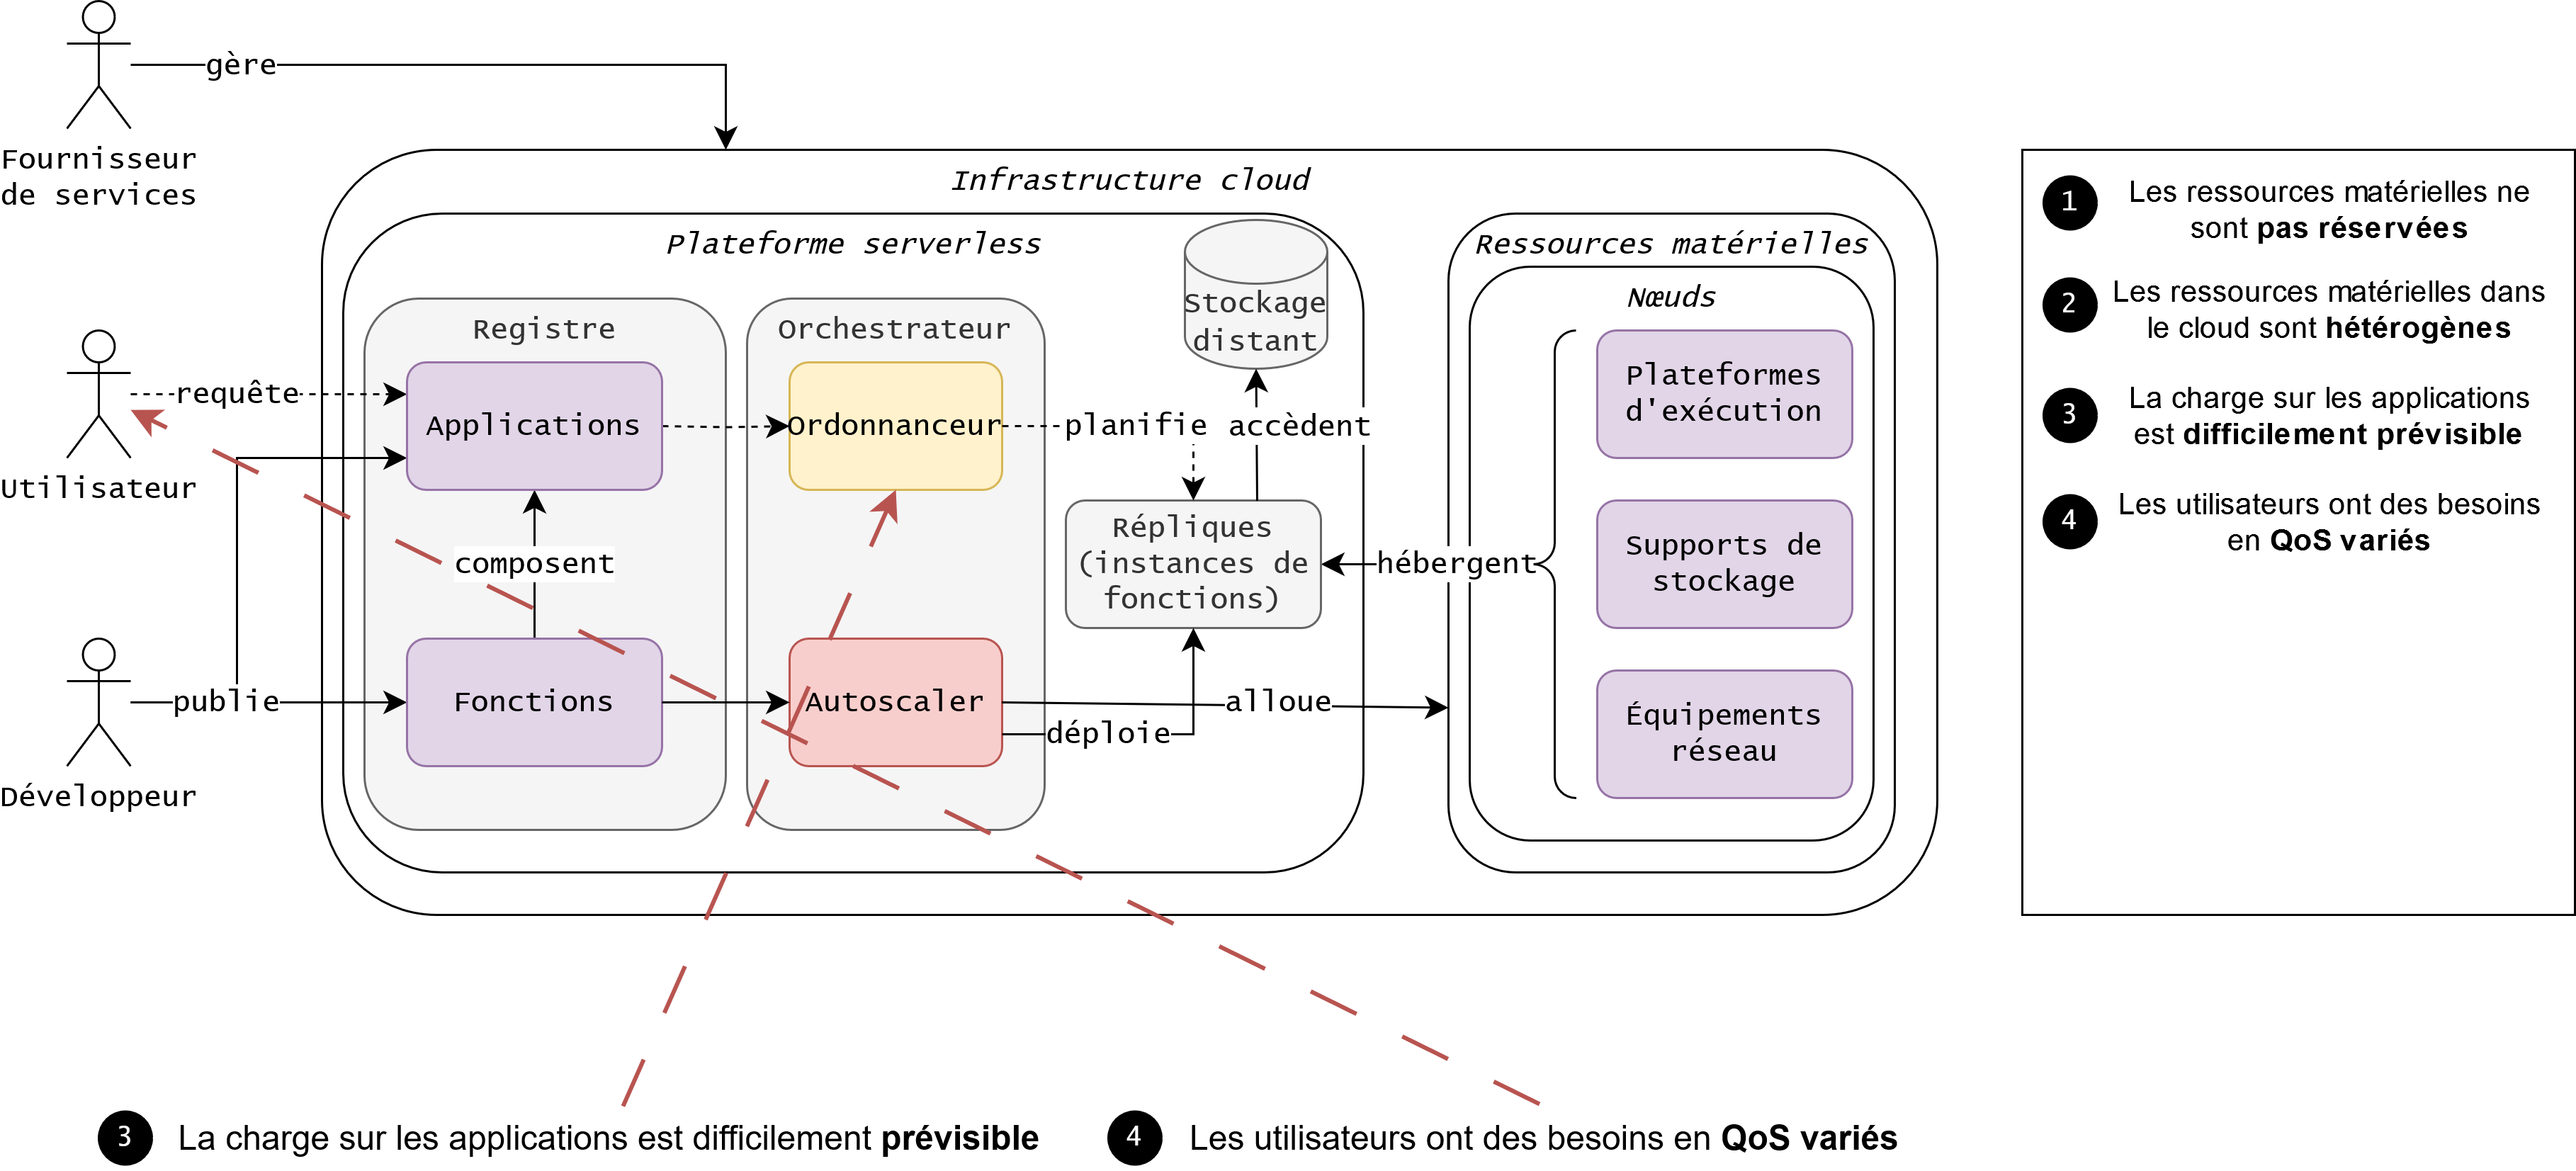
\includegraphics[width=\columnwidth]{img/sota-3.png}
    \end{center}

    \addtocounter{footnote}{1}
    \footnotetext{\fullcite{shahradServerlessWildCharacterizing}}
\end{frame}

\note[enumerate]{
    \item L'orchestration est un processus \textbf{en ligne}
    \item Cas d'usage sensibles au \textbf{débit} (tâches en lots) ou à la \textbf{latence} (applications interactives)
}

\begin{frame}[t,noframenumbering]{\textit{Serverless computing} : défis}
    \begin{center}
        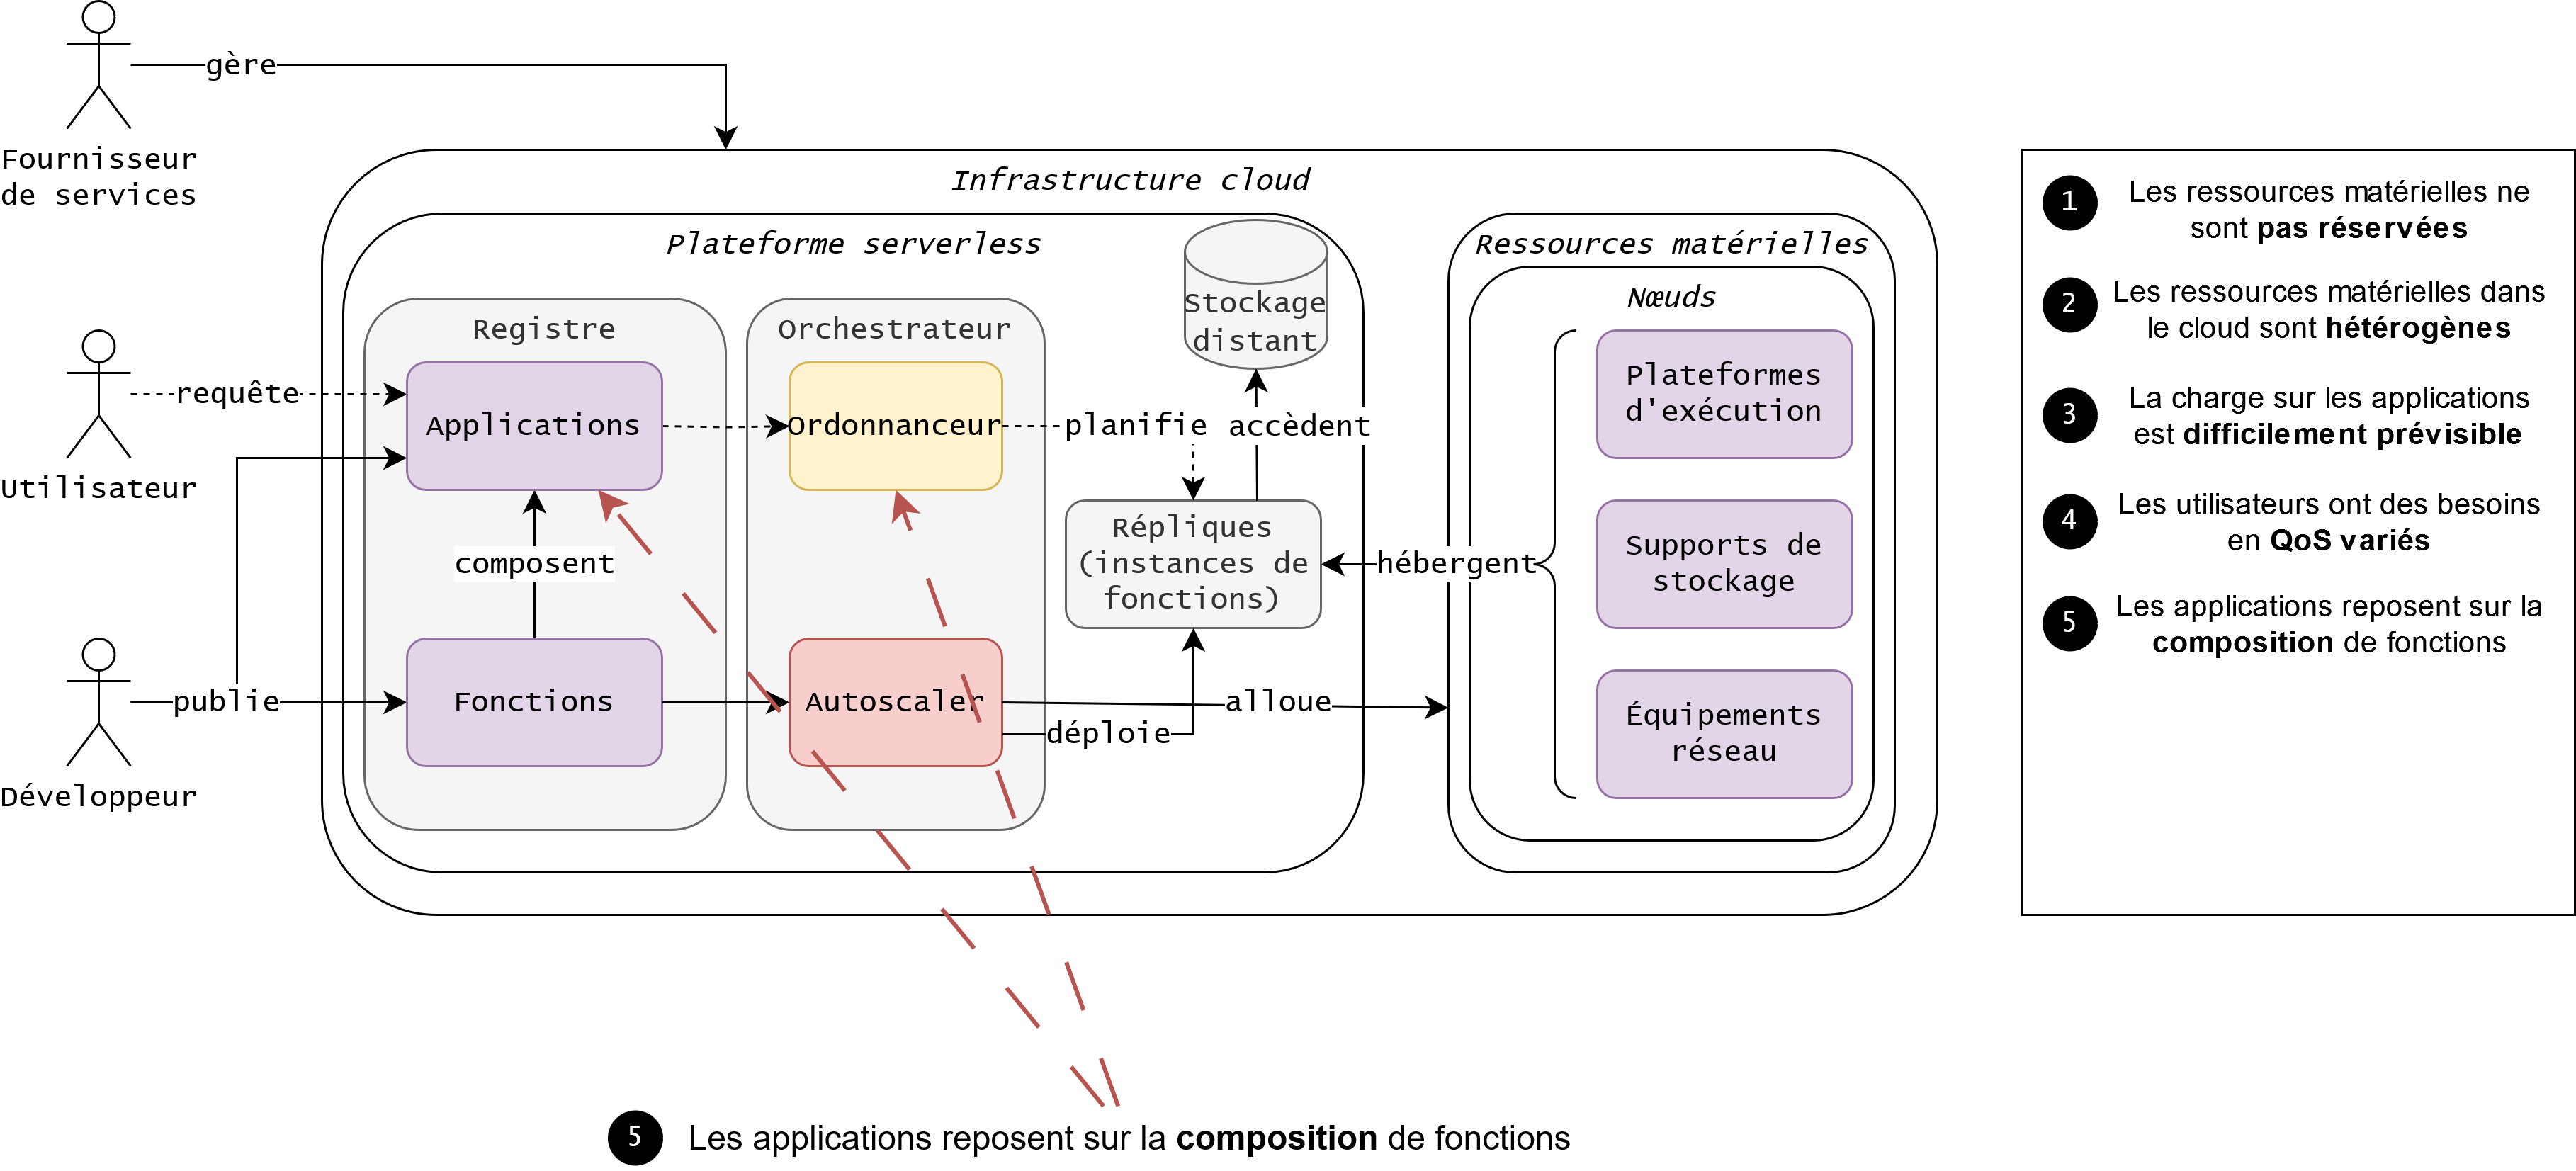
\includegraphics[width=\columnwidth]{img/sota-4.png}
    \end{center}

    \addtocounter{footnote}{1}
    \footnotetext{\fullcite{burckhardtNetheriteEfficientExecution}}
\end{frame}

\note[enumerate]{
    \item \textbf{Graphe acyclique} d'appels de fonctions
    \item Risque d'\textbf{effet boule de neige} sur la dégradation de la QoS
}

\begin{frame}[t,noframenumbering]{\textit{Serverless computing} : défis}
    \begin{center}
        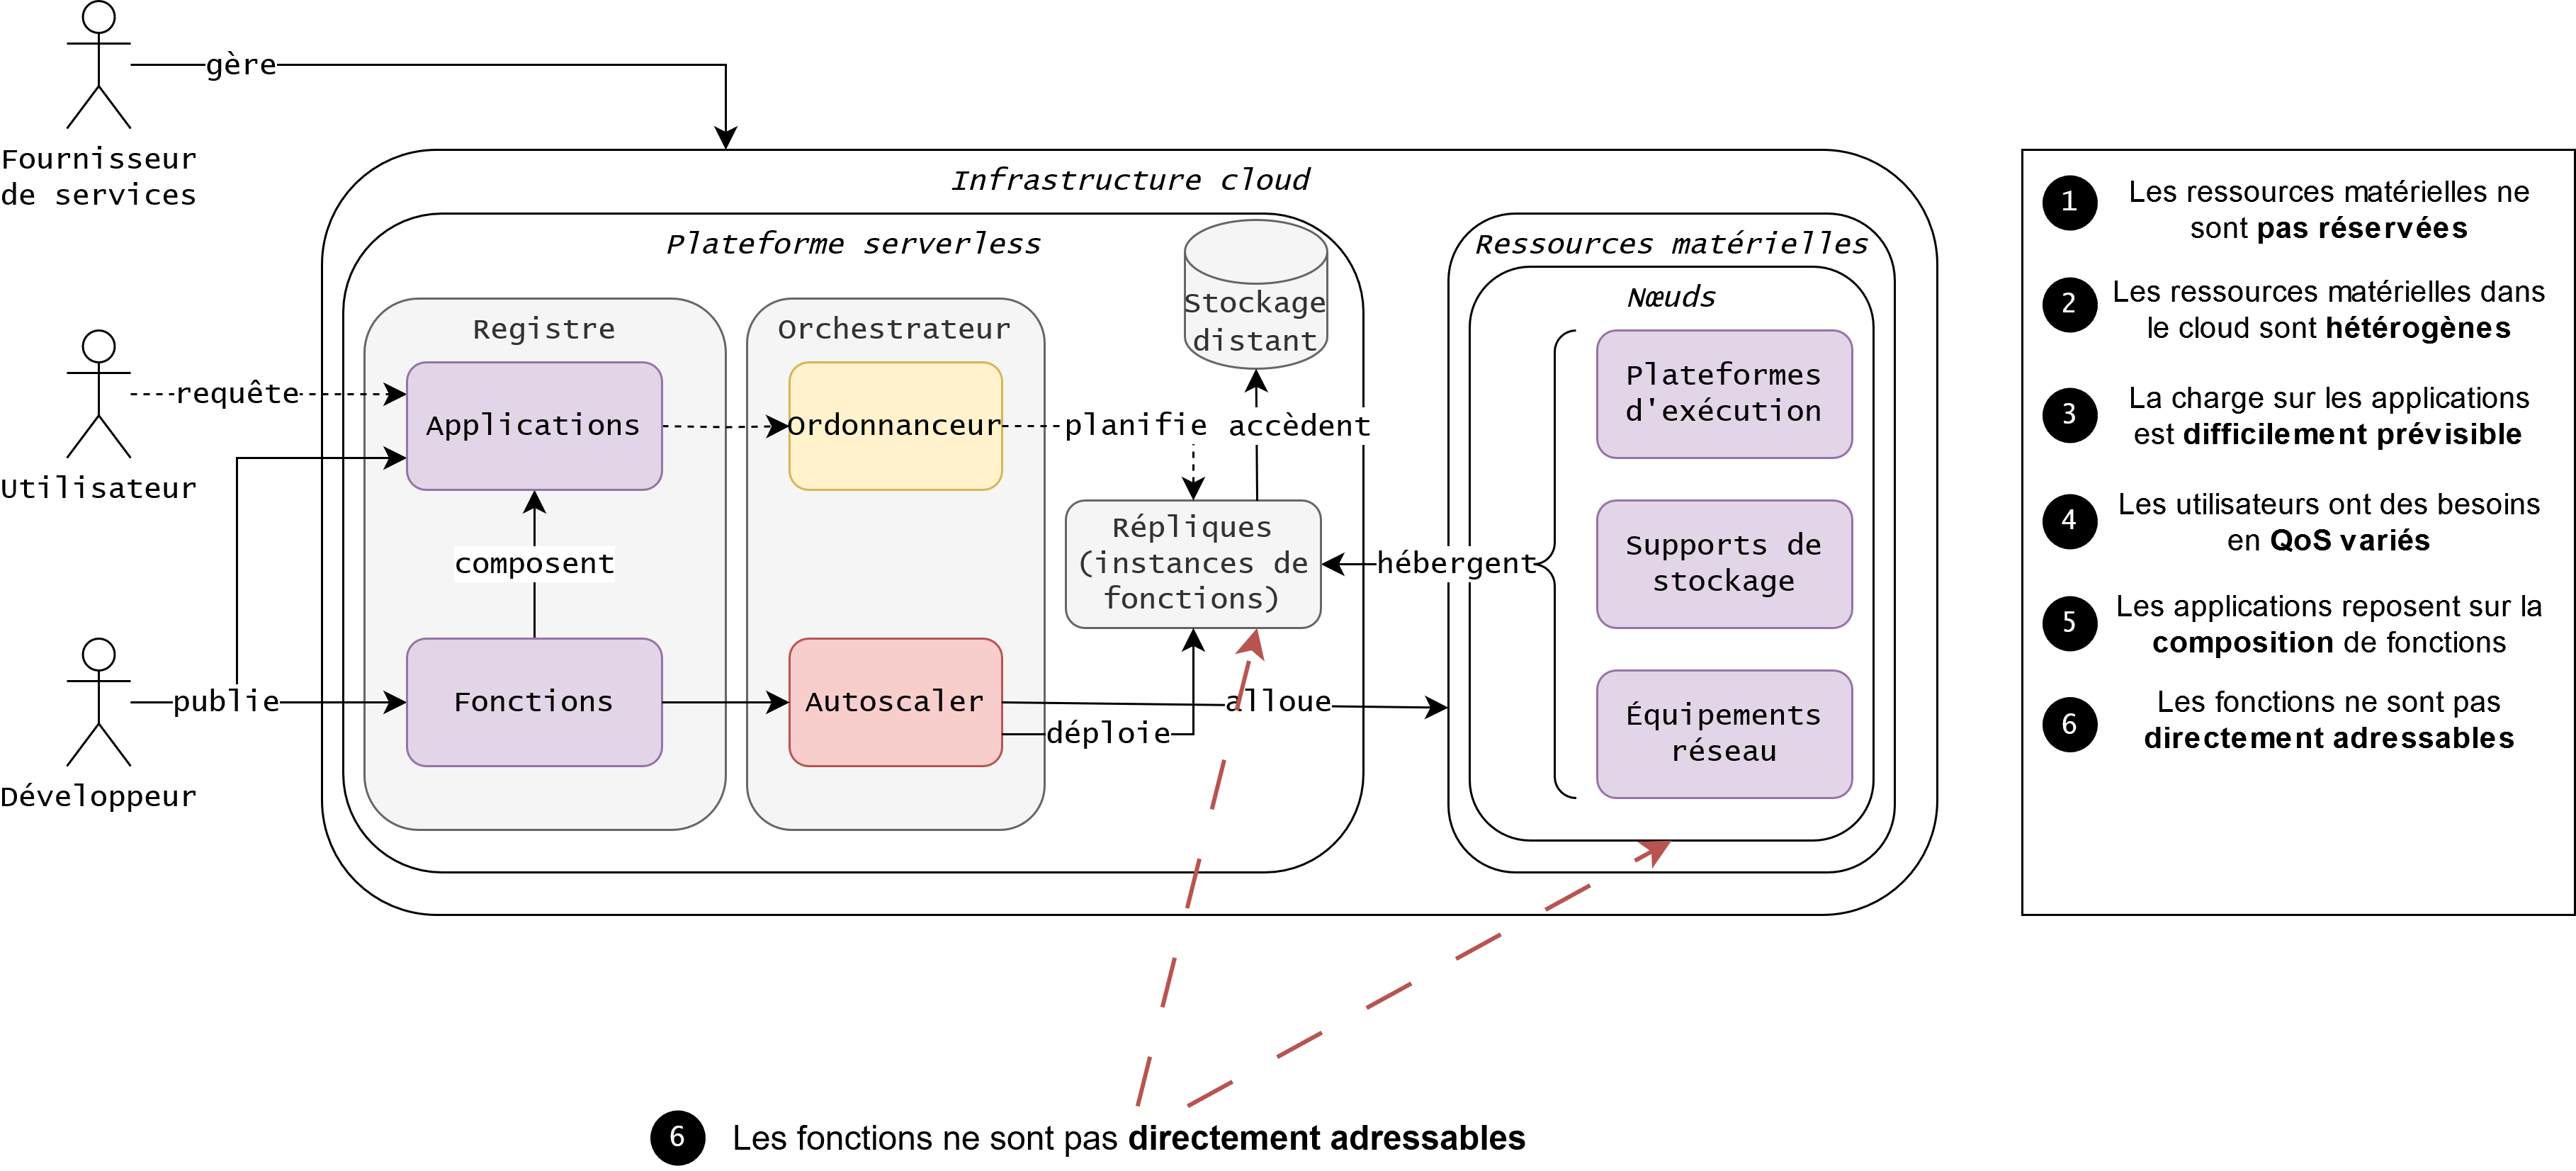
\includegraphics[width=\columnwidth]{img/sota-5.png}
    \end{center}

    \addtocounter{footnote}{1}
    \footnotetext{\fullcite{mullerLambadaInteractiveData2020}}
\end{frame}

\note[enumerate]{
    \item Une application peut être \textbf{répartie} sur plusieurs nœuds
    \item Certaines fonctions peuvent ne pas encore avoir été \textbf{instanciées}
}

\begin{frame}[t,noframenumbering]{\textit{Serverless computing} : défis}
    \begin{center}
        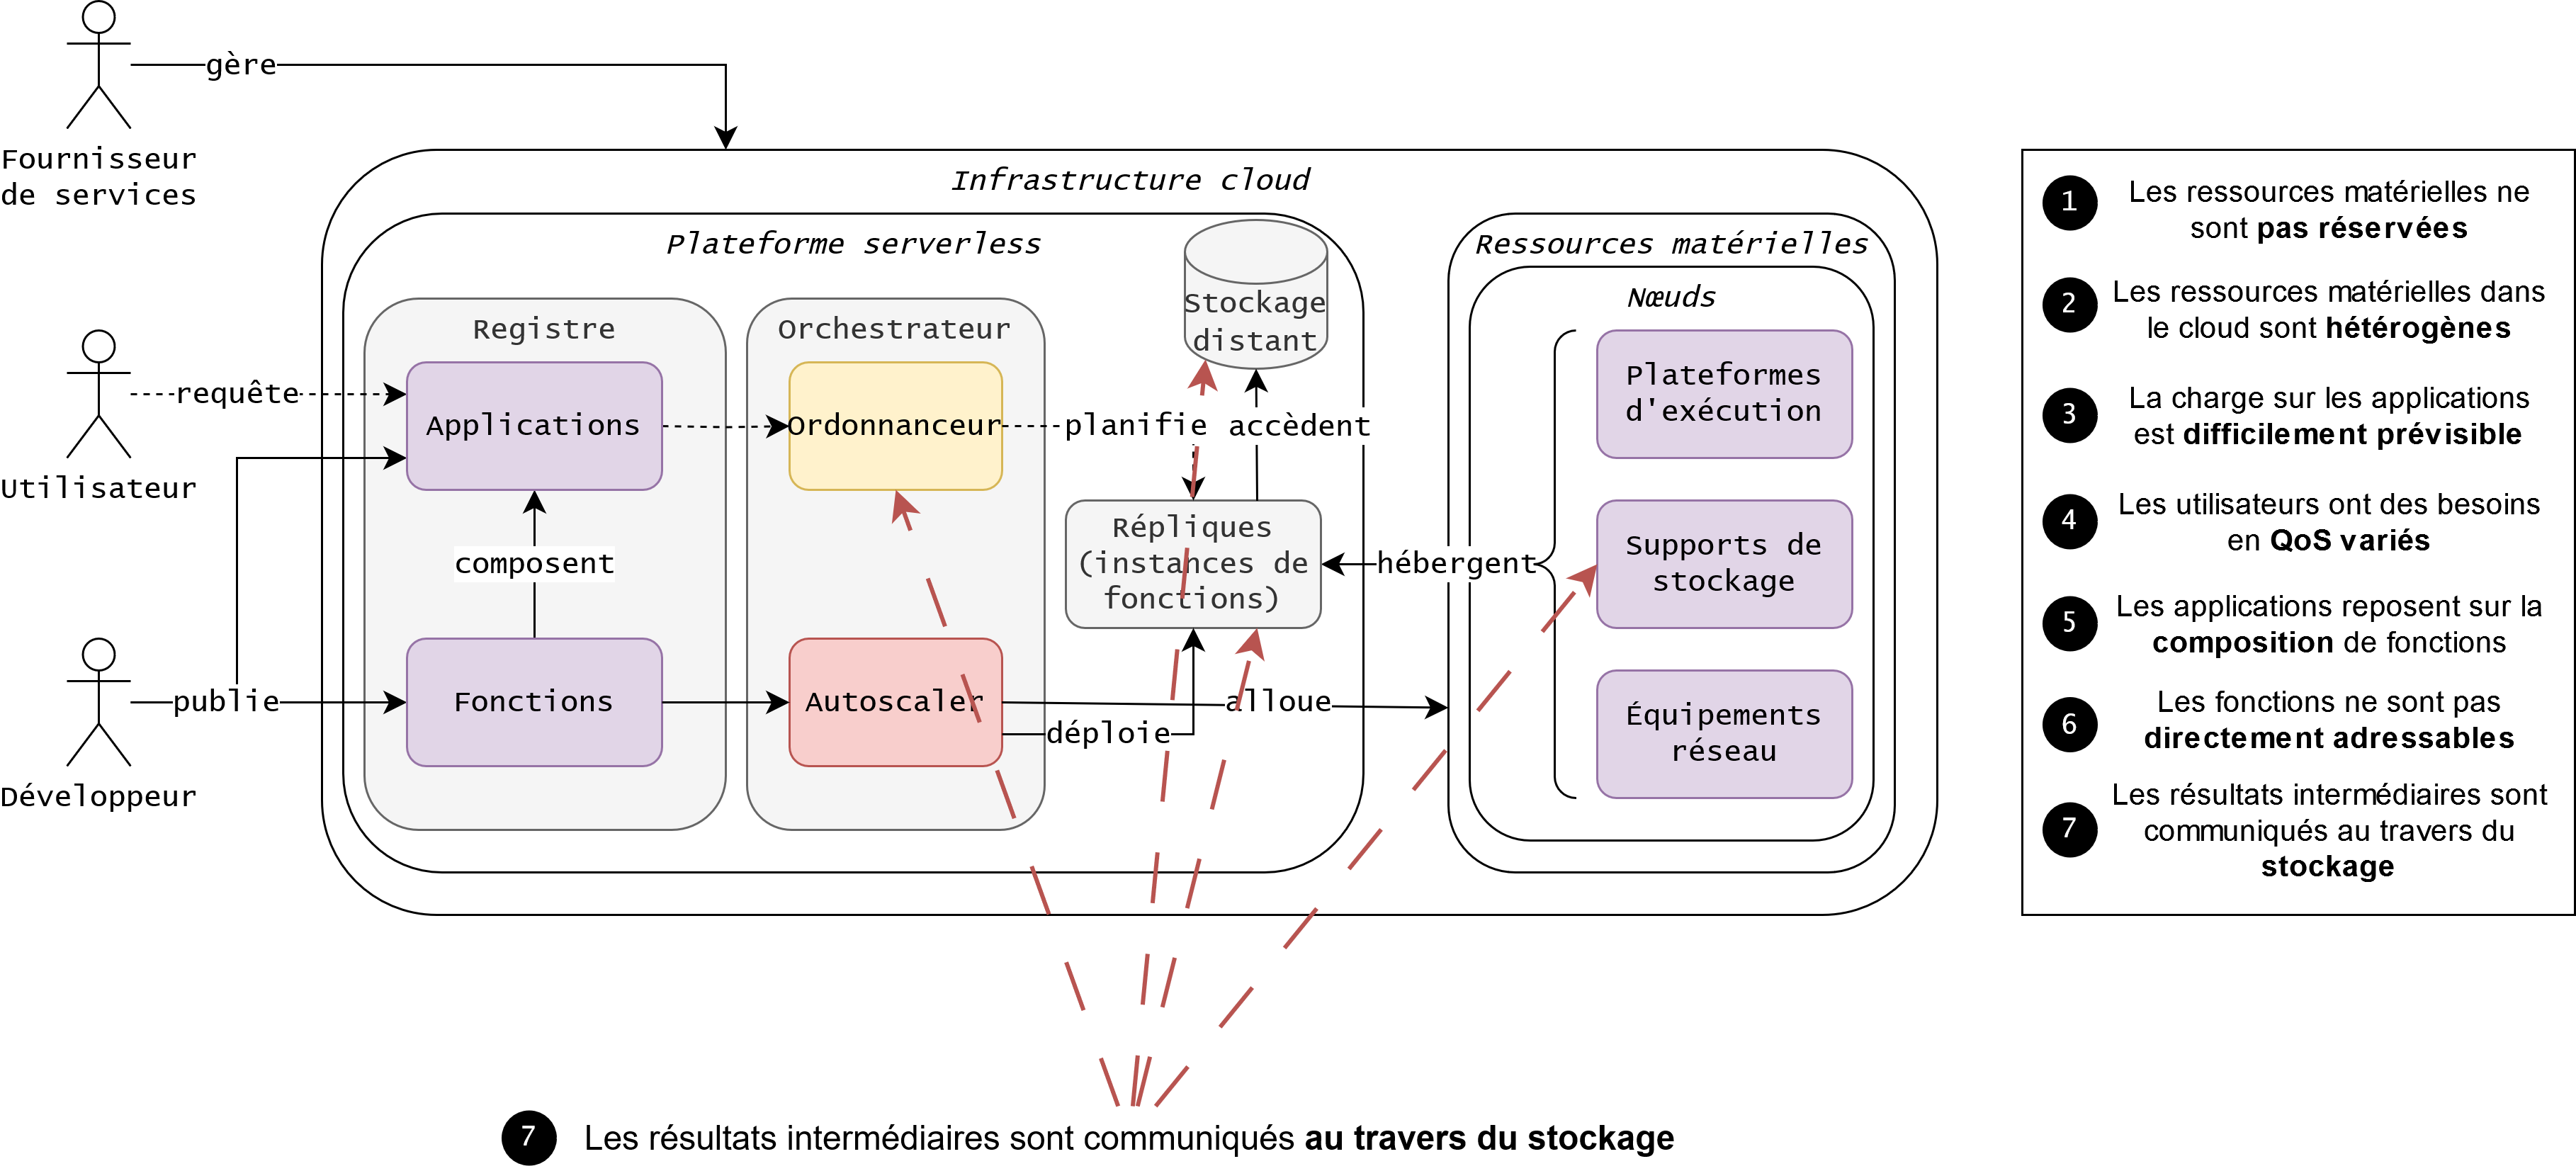
\includegraphics[width=\columnwidth]{img/sota-6.png}
    \end{center}

    \addtocounter{footnote}{1}
    \footnotetext{\fullcite{wawrzoniakBoxerDataAnalytics2021a}}
\end{frame}

\note[enumerate]{
    \item Local aux nœuds : risques de \textbf{contention}
    \item Accédé par le réseau : augmentation de la \textbf{latence}
}

\begin{framefont}{\small}
\begin{frame}{\textit{Serverless computing} : opportunités et menaces}
    \begin{center}
        \begin{table}[]
            \centering
            \begin{tabularx}{\textwidth}{ZZZZY}
                \toprule
                \addlinespace[0.5em]
                \textbf{Propriété} & \textbf{Défis} & \textbf{Opportunité} & \textbf{Menace} & \textbf{Contribution} \\
                \addlinespace[0.5em]
                \midrule
                \addlinespace[0.5em]
                \textbf{Dimensionnement dynamique} des ressources en fonction du besoin réel & 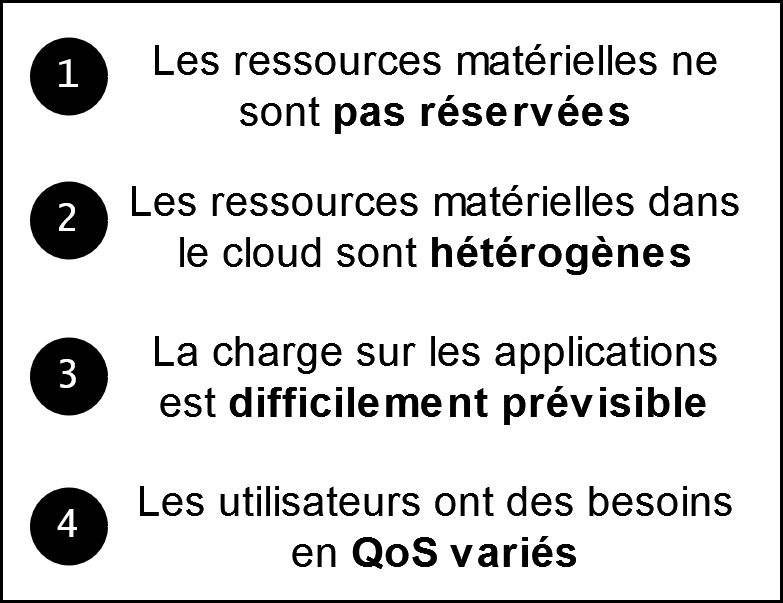
\includegraphics[width=0.2\textwidth]{img/problemes-1.png} & Optimisation de l'\textbf{utilisation des ressources} et de \textbf{l'énergie} & \textbf{Pics de latence} (démarrages à froid) & \textbf{HeROfake} \\
                \addlinespace[0.5em]
                % \midrule
                % \addlinespace[0.5em]
                \textbf{Placement dynamique} des requêtes utilisateur sur les répliques & 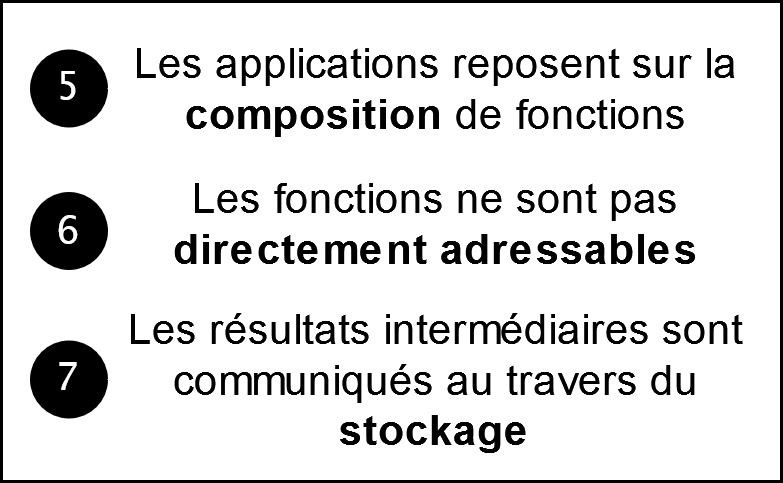
\includegraphics[width=0.2\textwidth]{img/problemes-2.png} & Respect de la \textbf{Qualité de Service} au plus proche des besoins & \textbf{Baisses de débit} (communications inter-fonctions) & \textbf{HeROcache} \\
                \addlinespace[0.5em]
                \bottomrule
            \end{tabularx}
        \end{table}
    \end{center}
\end{frame}
\end{framefont}

\note[enumerate]{
    \item Contributions : politiques d'orchestration qui mobilisent ces leviers pour atteindre des objectifs d'optimisation ;
    \item Troisième contribution : un environnement d'évaluation basé sur la mesure et la simulation.
}

\section{\textbf{HeROfake} -- Orchestrer des fonctions sur ressources hétérogènes dans le modèle serverless}

\begin{frame}{HeROfake -- Cas d'usage}
    \begin{columns}
        \column{0.5\textwidth}
        \resizebox{0.9\columnwidth}{!}{\vbox{
            \textbf{Cas d'usage : détection de deepfake}
            \begin{itemize}
                \item Détection à la demande, application dirigée par les événements ;
                \item Traitements sans état (images) ou avec état (vidéos).
            \end{itemize}
        
            \textbf{Détection de deepfake \textit{"as a service"}}
            \begin{itemize}
                \item Différents niveaux de Qualité de Service :
                \begin{itemize}
                    \item Utilisation par des particuliers (réseaux sociaux, etc.) ;
                    \item Usages critiques (autorités, médias) ;
                \end{itemize}
                \item Possibilité d'accélération à la demande (GPU, FPGA) ;
                \item Ressources partagées et contraintes.
            \end{itemize}
        }}
        
        \column{0.5\textwidth}
        \begin{center}
            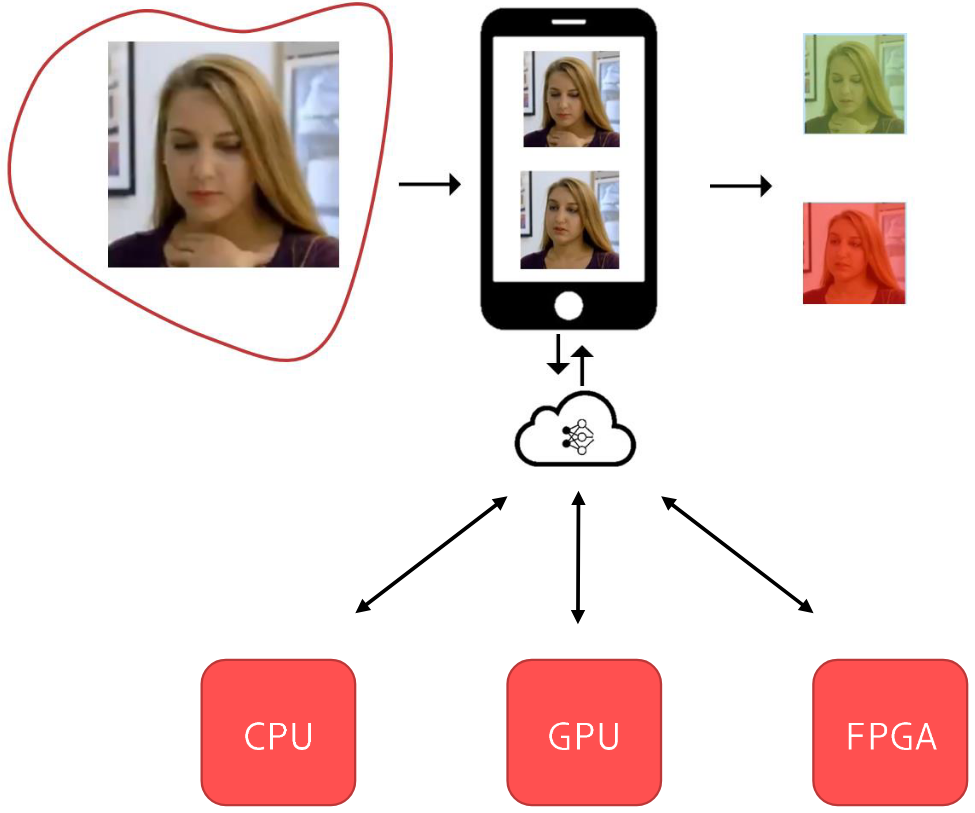
\includegraphics[width=\textwidth]{img/deepfake-service.png}
        \end{center}
    \end{columns}
\end{frame}

\begin{frame}{HeROfake -- Problème}
    \begin{exampleblock}{Question de recherche 1 (\textbf{QR1})}
        Comment \textbf{dimensionner les allocations} de ressources \textbf{hétérogènes} pour une application simple, constituée de fonctions de \textbf{courte durée}, et comment ordonnancer efficacement les requêtes des utilisateurs, lorsque ces derniers ont des besoins variés en matière de \textbf{qualité de service} ?
    \end{exampleblock}
\end{frame}

\begin{frame}{HeROfake -- Travaux connexes}
    \begin{table}[]
    \centering
    \caption{État de l'art des solutions de déploiement avec mise à l'échelle automatique pour des tâches de courte durée.}
    \resizebox{\textwidth}{!}{
        \begin{tabular}{lYYYYYYY}
            \toprule
            & Serverless & Déploiement cible & QoS & Hétérogénéité matérielle & Utilisation des ressources & Énergie & Conscient du coût \\
            \cmidrule(lr){2-2}\cmidrule(lr){3-3}\cmidrule(lr){4-4}\cmidrule(lr){5-5}\cmidrule(lr){6-6}\cmidrule(lr){7-7}\cmidrule(lr){8-8}
            Swayam~\cite{gujaratiSwayamDistributedAutoscaling2017} & \xmark & Public (Azure) & \cmark & \xmark & \cmark & \xmark & \xmark \\
            Pigeon~\cite{lingPigeonDynamicEfficient2019} & \cmark & Privé & \xmark & \cmark & \cmark & \xmark & \xmark \\
            MArk~\cite{zhangMArkExploitingCloud} & \xmark & Public (AWS) & \cmark & \cmark & \cmark & \xmark & \cmark \\
            ENSURE~\cite{sureshENSUREEfficientScheduling2020} & \cmark & Privé & \xmark & \xmark & \cmark & \xmark & \cmark \\
            Mampage et al.~\cite{mampageDeadlineawareDynamicResource2021} & \cmark & Privé & \cmark & \xmark & \cmark & \xmark & \cmark \\
            Atoll~\cite{singhviAtollScalableLowLatency2021} & \cmark & Privé & \cmark & \xmark & \xmark & \xmark & \xmark \\
            INFless~\cite{yangINFlessNativeServerless2022} & \cmark & Privé & \cmark & \xmark & \cmark & \xmark & \cmark \\
            SMIF~\cite{choSLADrivenMLInference} & \cmark & Privé & \cmark & \cmark & \cmark & \xmark & \xmark \\
            \textbf{Solution cible} & \cmark & Privé & \cmark & \cmark & \cmark & \cmark & \cmark \\ \bottomrule
        \end{tabular}
    }
    \label{table:sota-herofake-sota}
    \end{table}
\end{frame}

\begin{frame}{HeROfake -- Système considéré}
    \begin{columns}
        \column{0.5\textwidth}
        \resizebox{0.8\columnwidth}{!}{\vbox{
            \textbf{Caractérisation des fonctions (hors-ligne)}
            \begin{itemize}
                \item Générer des métadonnées pour les fonctions
                \item Utiles pour guider les décisions d'allocation et d'ordonnancement
            \end{itemize}
        }}

        \column{0.5\textwidth}
        \resizebox{0.8\columnwidth}{!}{\vbox{
            \textbf{Orchestration des fonctions (en ligne)}
            \begin{itemize}
                \item Allocation des ressources au plus près des besoins
                \item Éviter les violations de QoS
                \item Minimiser la consommation d'énergie
            \end{itemize}
        }}
    \end{columns}

    \begin{center}
        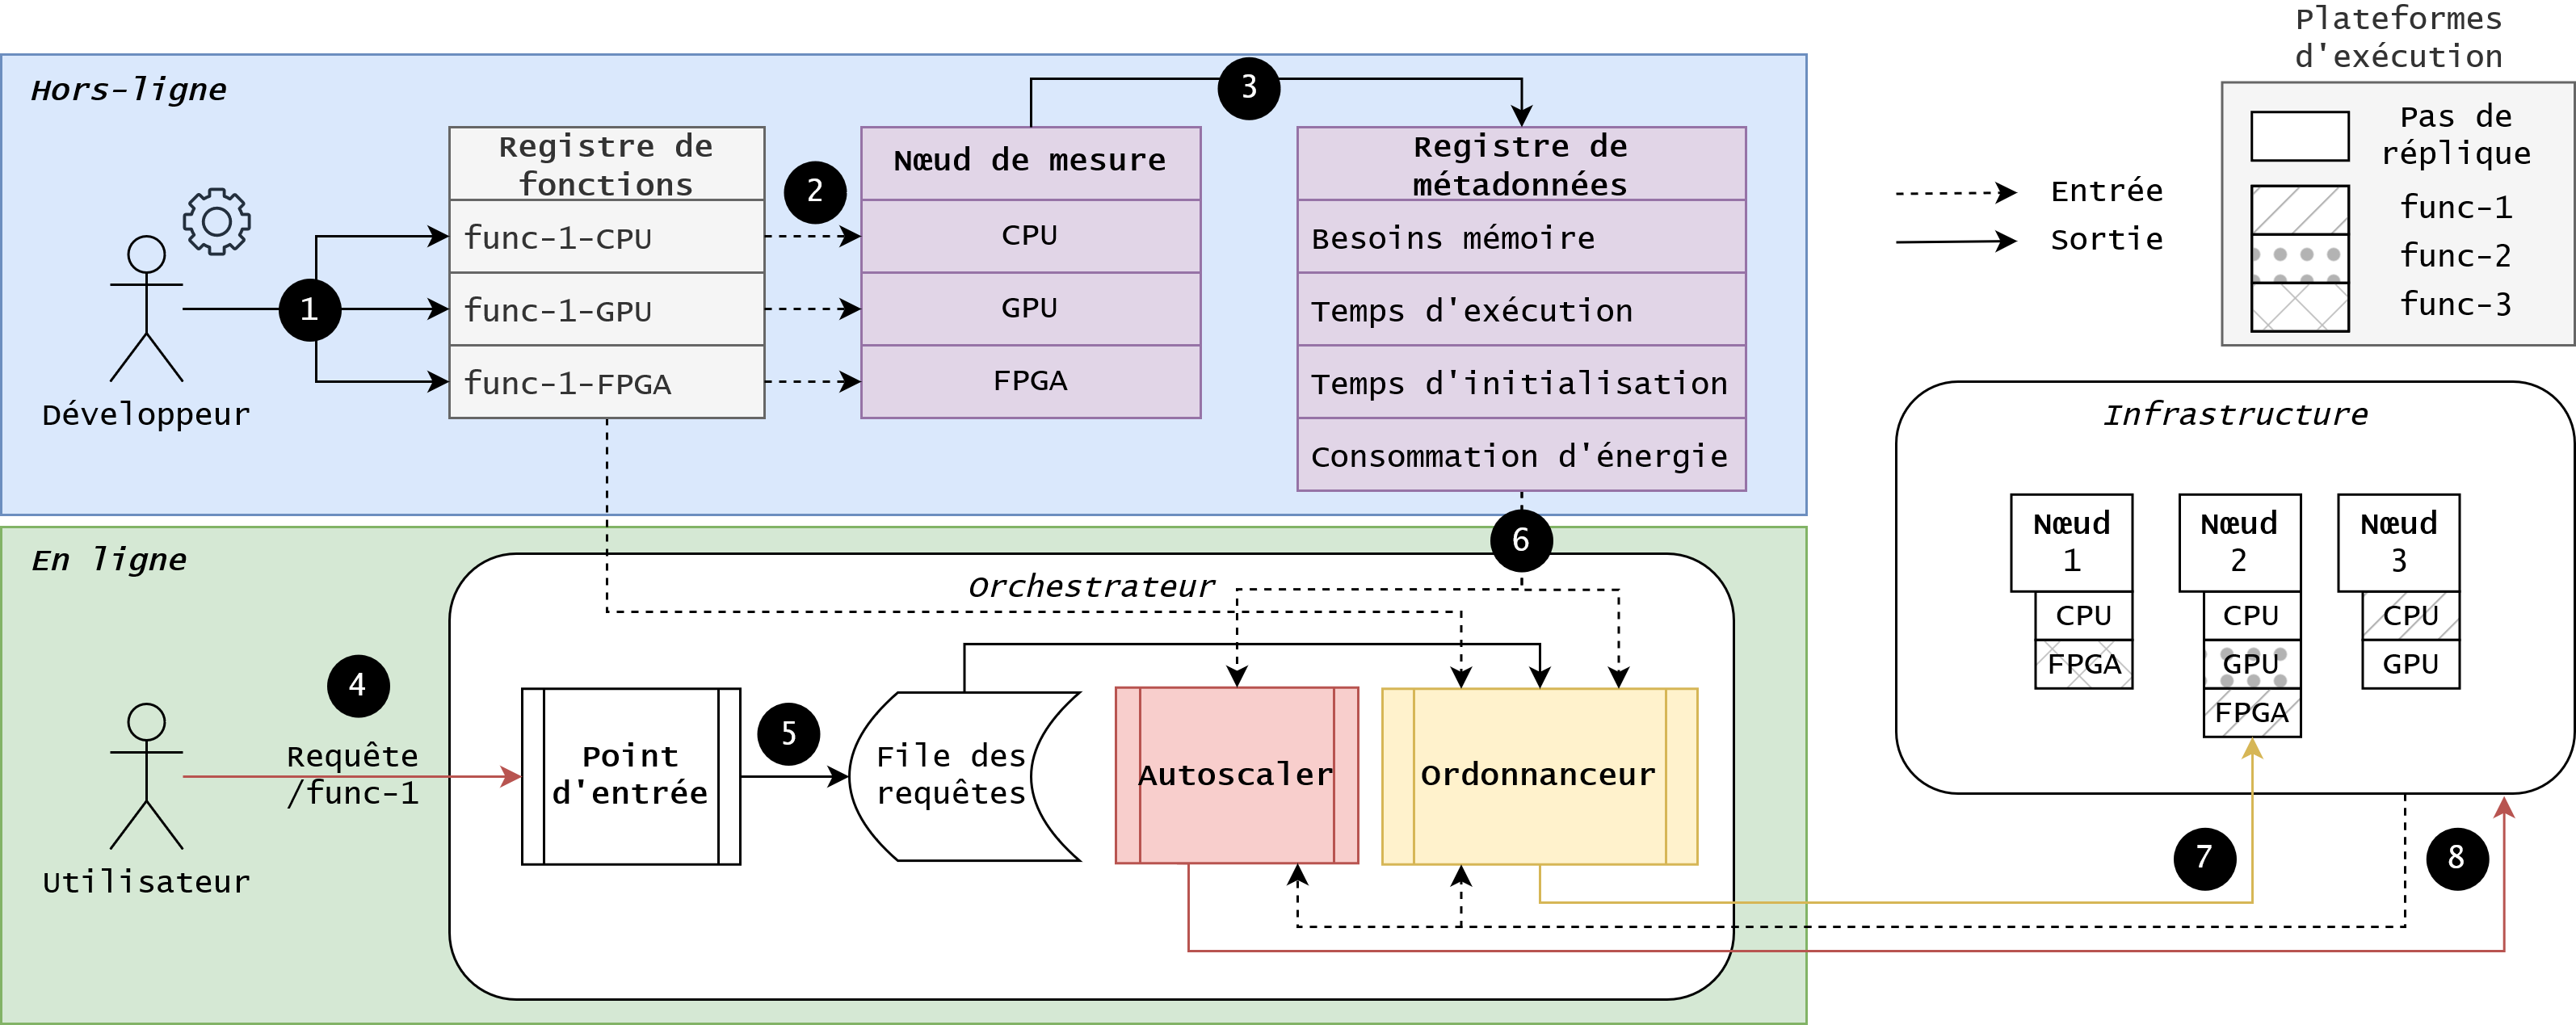
\includegraphics[width=0.8\columnwidth]{img/herofake-plateforme.png}
    \end{center}
\end{frame}

\begin{frame}{HeROfake -- Contribution : Mise à l'échelle dynamique}
    \begin{columns}
        \column{0.55\textwidth}
        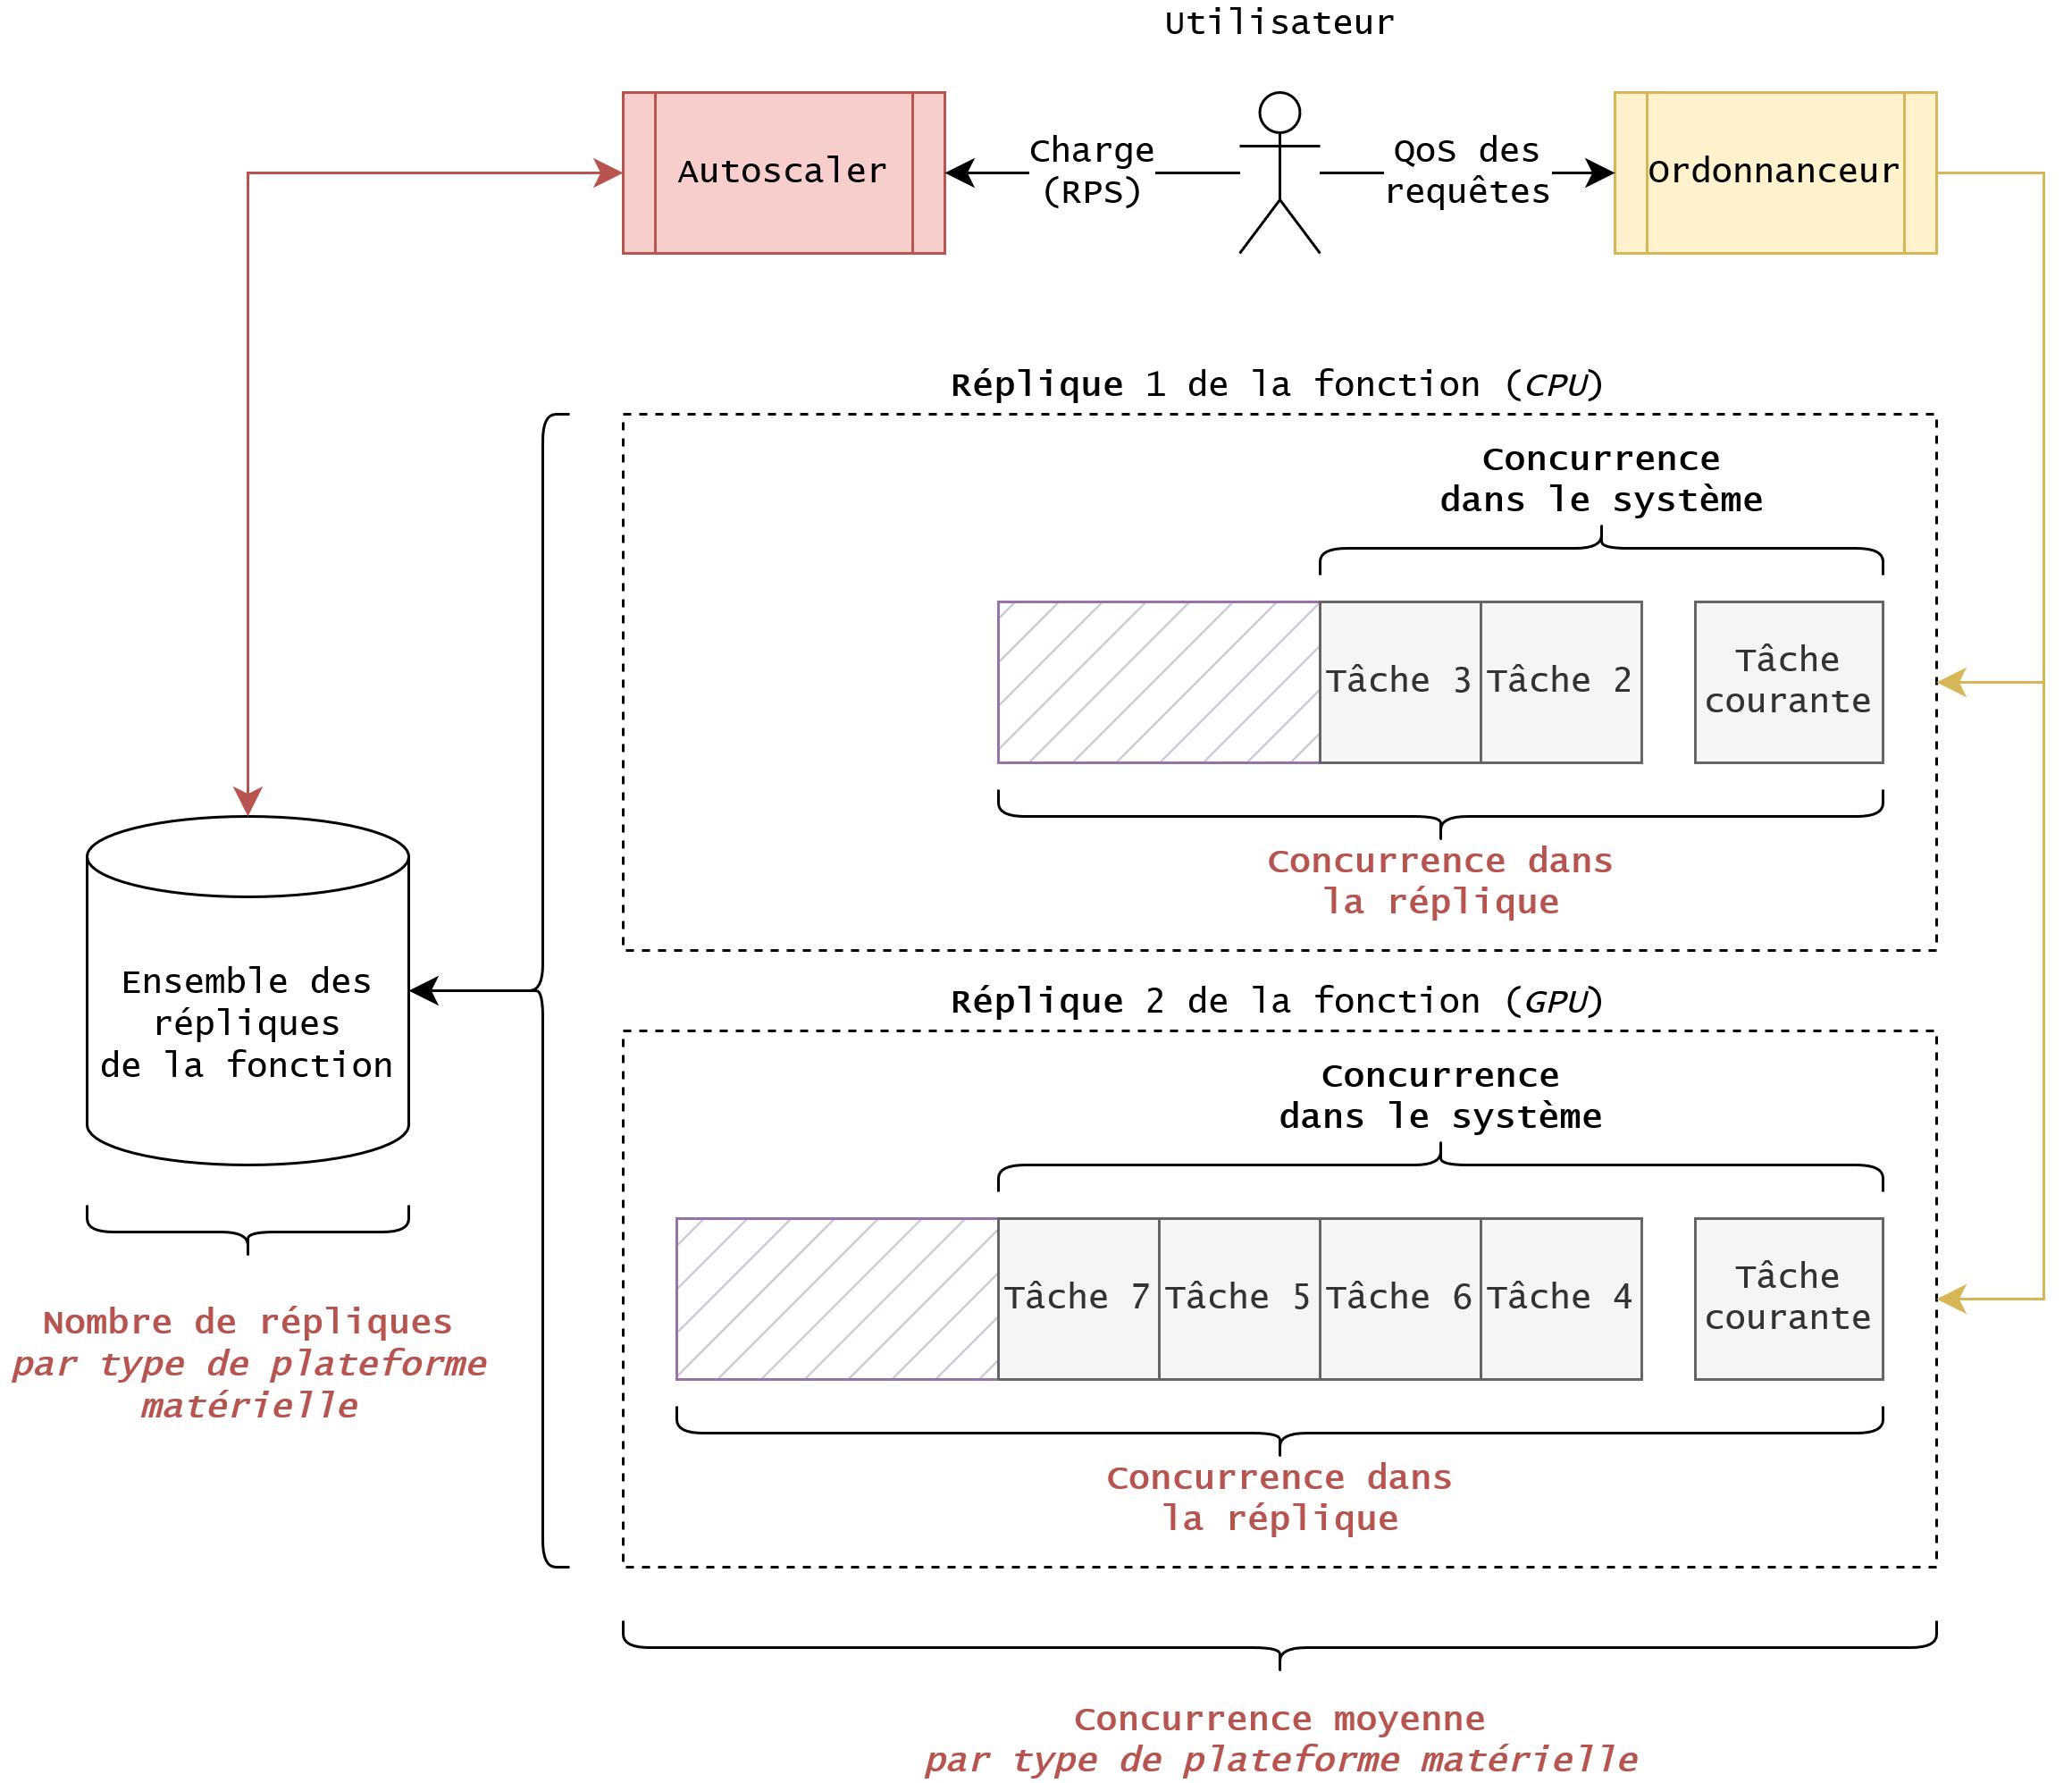
\includegraphics[width=0.95\columnwidth]{img/herofake-orchestration.png}

        \column{0.45\textwidth}
        \resizebox{0.85\columnwidth}{!}{\vbox{
            Knative~\footnotemark{}, répliques homogènes :
            
            \begin{equation*}
                replicaCount_{f} = \frac{inSystemConcurrency_{f}}{\textcolor{blue}{concurrencyTarget_{f}}}
            \end{equation*}
        
            Hétérogénéité matérielle :
            
            \begin{equation*}
                replicaCount_{{f}_{h}} = \frac{inSystemConcurrency_{{f}_{h}}}{\textcolor{red}{concurrencyTarget_{{f}_{h}}}}
            \end{equation*}
    
            Ratio composite pour seuil de concurrence :
    
            \begin{equation*}
                \textcolor{red}{cT_{f, h}} = \textcolor{blue}{cT_{f, c}} \cdot (k_{ET} \cdot \frac{ET_{{f}_{c}}}{ET_{{f}_{h}}} + k_{EC} \cdot \frac{EC_{{f}_{c}}}{EC_{{f}_{h}}} + k_{HP} \cdot \frac{HP_{{f}_{c}}}{HP_{{f}_{h}}})
            \end{equation*}
        }}
    \end{columns}

    \footnotetext{\fullcite{knative-autoscaling}}
\end{frame}

\note[enumerate]{
    \item Mise à l'échelle : verticalement, horizontalement (serverless)
    \item On considère un orchestrateur dans lequel les requêtes utilisateur sont positionnées en file d'attente dans les répliques (ré-utilisation des répliques, par opposition à 1 requête = 1 réplique)
    \item Ajuster la taille des files d'attente permet de jouer sur le nombre de démarrages à froid (à intensité de trafic égale)
}

\begin{frame}{HeROfake -- Contribution : Stratégie de minimisation des coûts}
    \begin{columns}
        \column{0.6\textwidth}
        \begin{itemize}
            \item \textbf{Autoscaling}
            \begin{itemize}
                \item \textbf{Minimiser} le coût des \textcolor{blue}{démarrages à froid}, la consommation d'\textcolor{orange}{énergie} et le coût de \textcolor{purple}{possession} total :
            \end{itemize}

            \resizebox{0.85\columnwidth}{!}{\vbox{
                \begin{center}
                    \begin{equation*}
                        \begin{split}
                            \forall N, \forall P \in N, \, scaleCost_{{f}_{N, P}} = \,
                                  &k_{TT} \cdot {TT}_{{f}_{N, P}} \\
                                + &k_{EC} \cdot \textcolor{orange}{{EC}_{{f}_{N, P}}} \\
                                + &k_{HP} \cdot \textcolor{purple}{{HP}_{{f}_{N, P}}}
                    \end{split}
                    \end{equation*}
                \end{center}
            }}

            \item \textbf{Ordonnancement}
            \begin{itemize}
                \item \textbf{Minimiser} les \textcolor{red}{pénalités} sur QoS, la consommation d'\textcolor{orange}{énergie} et la \textcolor{teal}{dispersion} des tâches :
            \end{itemize}

            \resizebox{0.85\columnwidth}{!}{\vbox{
                \begin{center}
                    \begin{equation*}
                        \begin{split}
                            \forall (N, P) \in R_{f}, \, schedCost_{{f}_{N, P}} = \,
                                  &k_{QP} \cdot \textcolor{red}{{QP}_{{f}_{N, P}}} \\
                                + &k_{EC} \cdot \textcolor{orange}{{EC}_{{f}_{N, P}}} \\
                                + &k_{TC} \cdot \textcolor{teal}{{TC}_{{f}_{N, P}}}
                        \end{split}
                    \end{equation*}
                \end{center}
            }}
        \end{itemize}

        \column{0.4\textwidth}
        Mobiliser les métadonnées issues de la phase de caractérisation :

        \begin{center}
            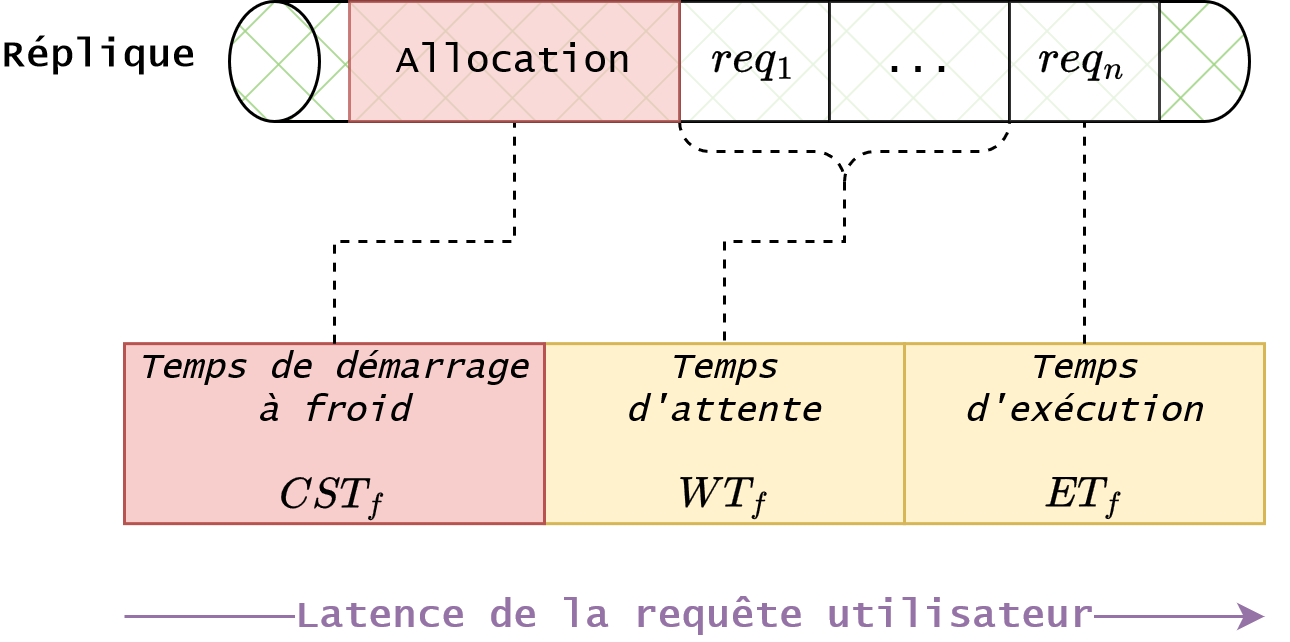
\includegraphics[width=\columnwidth]{img/herofake-total-time.png}
        \end{center}

        \begin{equation*}
            {TT}_{{f}_{N, P}} = \textcolor{blue}{{CST}_{{f}_{N, P}}} + {WT}_{{f}_{N, P}} + {ET}_{{f}_{N, P}}
        \end{equation*}
    \end{columns}
\end{frame}

\note[enumerate]{
    \item Les coefficients $k$ sont configurables par le fournisseur de services, pour donner un poids différent à chacune des composantes du coût en fonction de ses contraintes propres
}

\begin{framefont}{\footnotesize}
\begin{frame}[t]{HeROfake -- Évaluation : Méthodologie}
    \begin{columns}
        \column{0.5\textwidth}
        Évaluation en deux phases :
        \begin{itemize}
            \item \textbf{Comparaison aux politiques de référence}
            \item \textbf{Impact des différents composants}
        \end{itemize}

        Infrastructure retenue :
        \begin{itemize}
            \item 10 nœuds (10 CPUs, 6 GPUs, 2 FPGAs) ;
        \end{itemize}

        Scénario d'évaluation :
        \begin{itemize}
            \item 50 000 requêtes ;
            \item 50 à 100 requêtes par seconde ;
            \item Distribution uniforme des niveaux de QoS requis.
        \end{itemize}

        \column{0.5\textwidth}
        \textbf{Autoscalers} :

        \begin{itemize}
            \item HeROfake (\textbf{HRO}) -- Conscience de l'hétérogénéité matérielle pour les performances et la consommation d'énergie ;
            \item Knative (\textbf{KN}) -- Sélection du nœud le plus disponible, \textit{i.e.} équilibrage de charge.
        \end{itemize}

        \textbf{Ordonnanceurs} :

        \begin{itemize}
            \item HeROfake (\textbf{HRO}) -- Conscience de l'hétérogénéité matérielle et des échéances pour le respect de la QoS ;
            \item Knative (\textbf{KN}) -- Répliques homogènes, sélection par file d'attente la plus courte~\footnotemark{} ;
            \item Bin-Packing First Fit (\textbf{BPFF}) -- Ordonnanceur dans AWS Lambda, sélection par file d'attente la plus chargée~\footnotemark{} ;
            \item Random Placement (\textbf{RP}) -- Sélection d'une réplique aléatoire.
        \end{itemize}
    \end{columns}

    \addtocounter{footnote}{1}
    \footnotetext{\fullcite{sureshENSUREEfficientScheduling2020}}
    \addtocounter{footnote}{1}
    \footnotetext{\fullcite{wangPeekingCurtainsServerlessb}}
\end{frame}
\end{framefont}

\begin{frame}{HeROfake -- Évaluation : Analyse des résultats i}
    \begin{center}
        \resizebox{0.8\columnwidth}{!}{\vbox{
            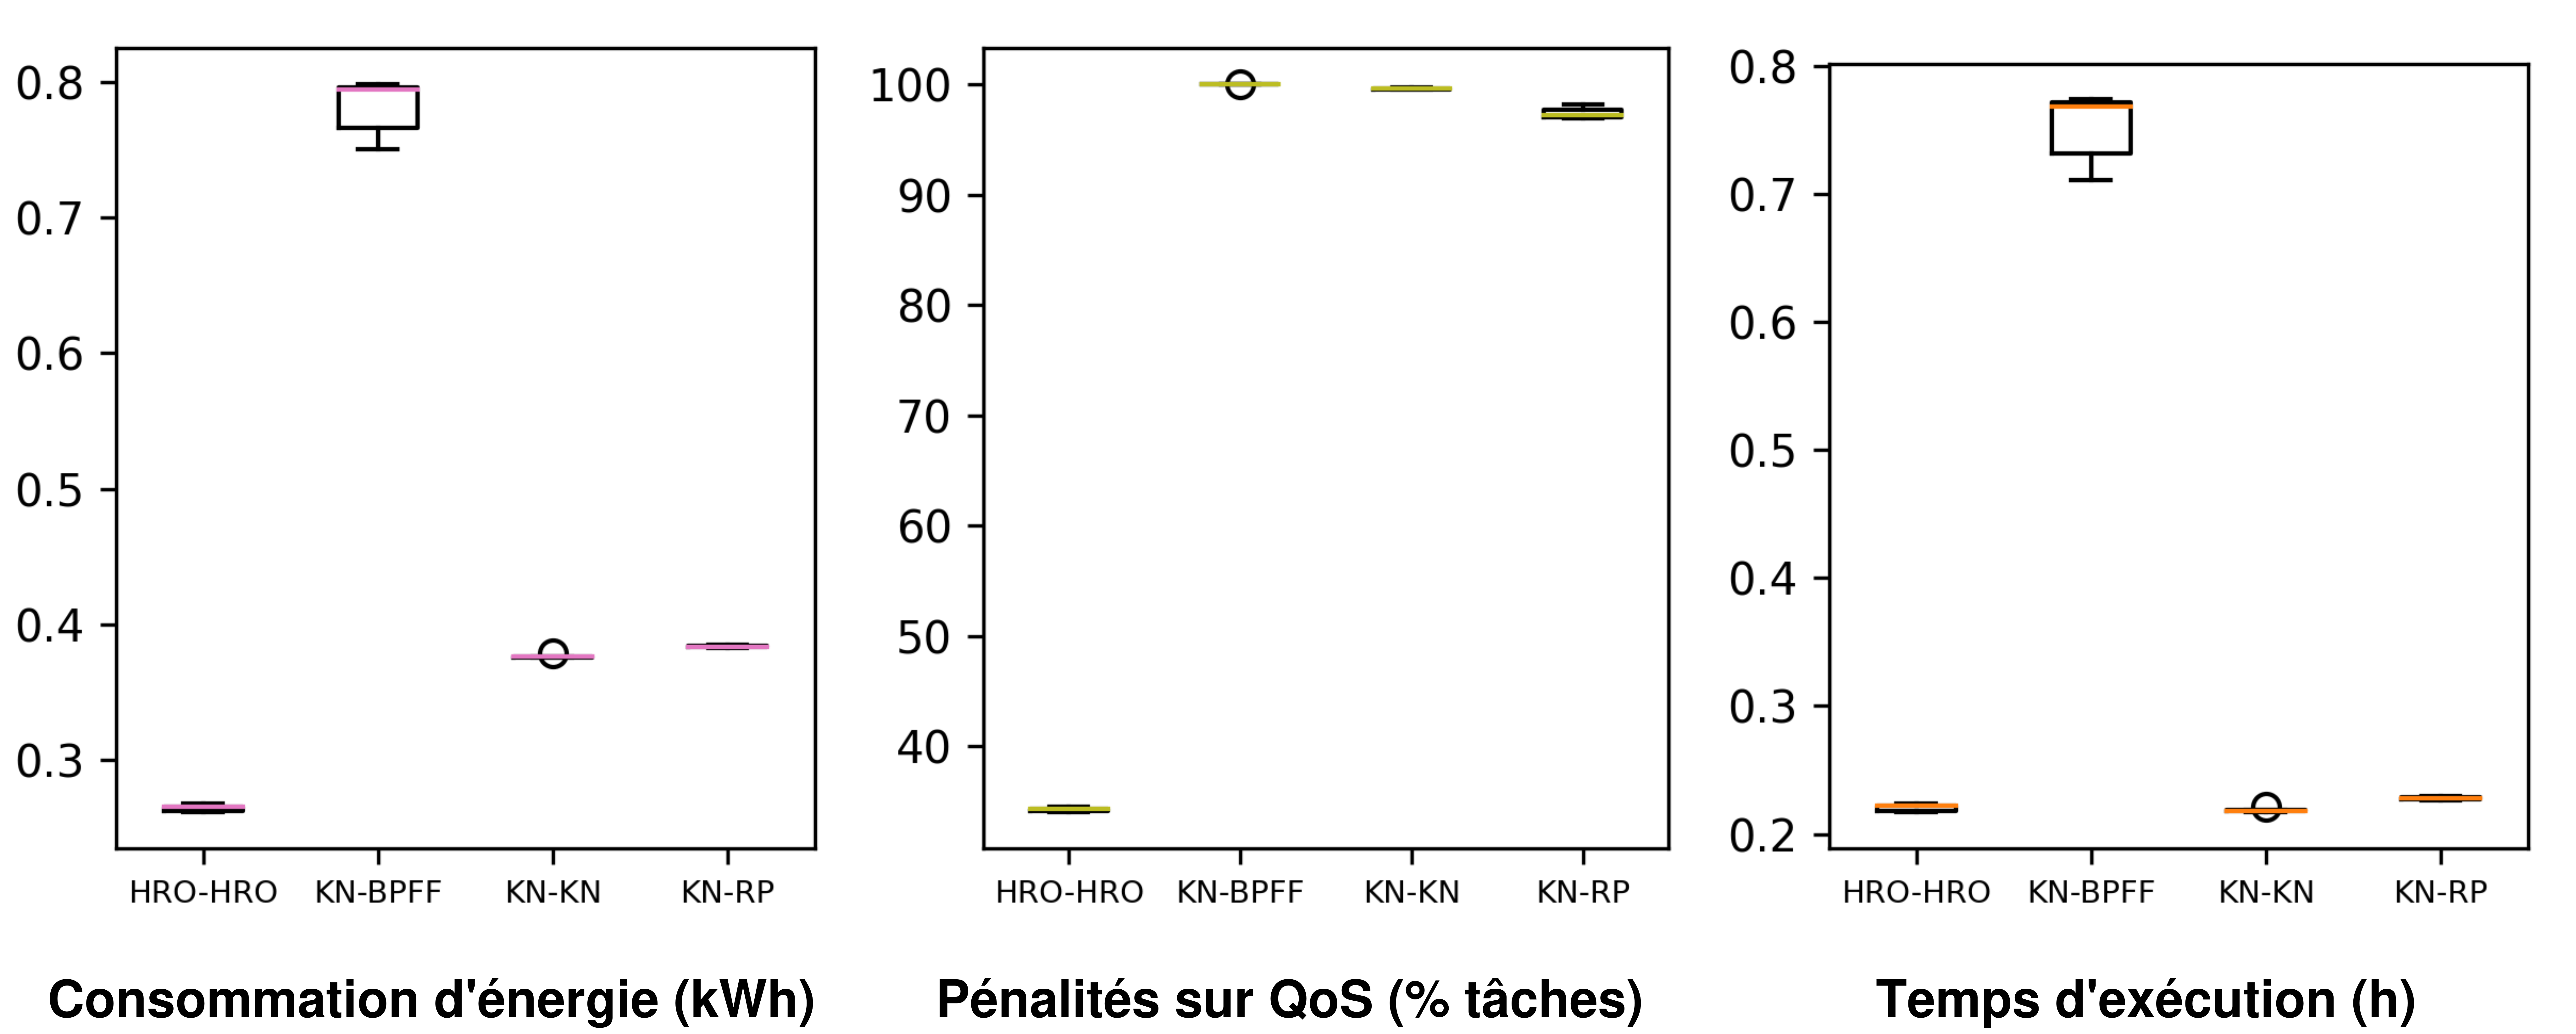
\includegraphics[width=\columnwidth]{img/eval-herofake/herofake-resultats-1.png}
        }}
    \end{center}
\end{frame}

\note[enumerate]{
    \item Consolidation (BPFF) : plus grand temps d'exécution, plus grande consommation d'énergie ;
    \item HeROfake donne une consommation d'énergie plus faible car la politique mobilise les accélérateurs matériels ;
    \item Malgré des démarrages à froid plus longs, ces accélérateurs permettent d'accélérer le traitement des requêtes à haute priorité : réduction des pénalités sur QoS.
}

\begin{frame}{HeROfake -- Évaluation : Analyse des résultats ii}
    \begin{center}
        \resizebox{0.8\columnwidth}{!}{\vbox{
            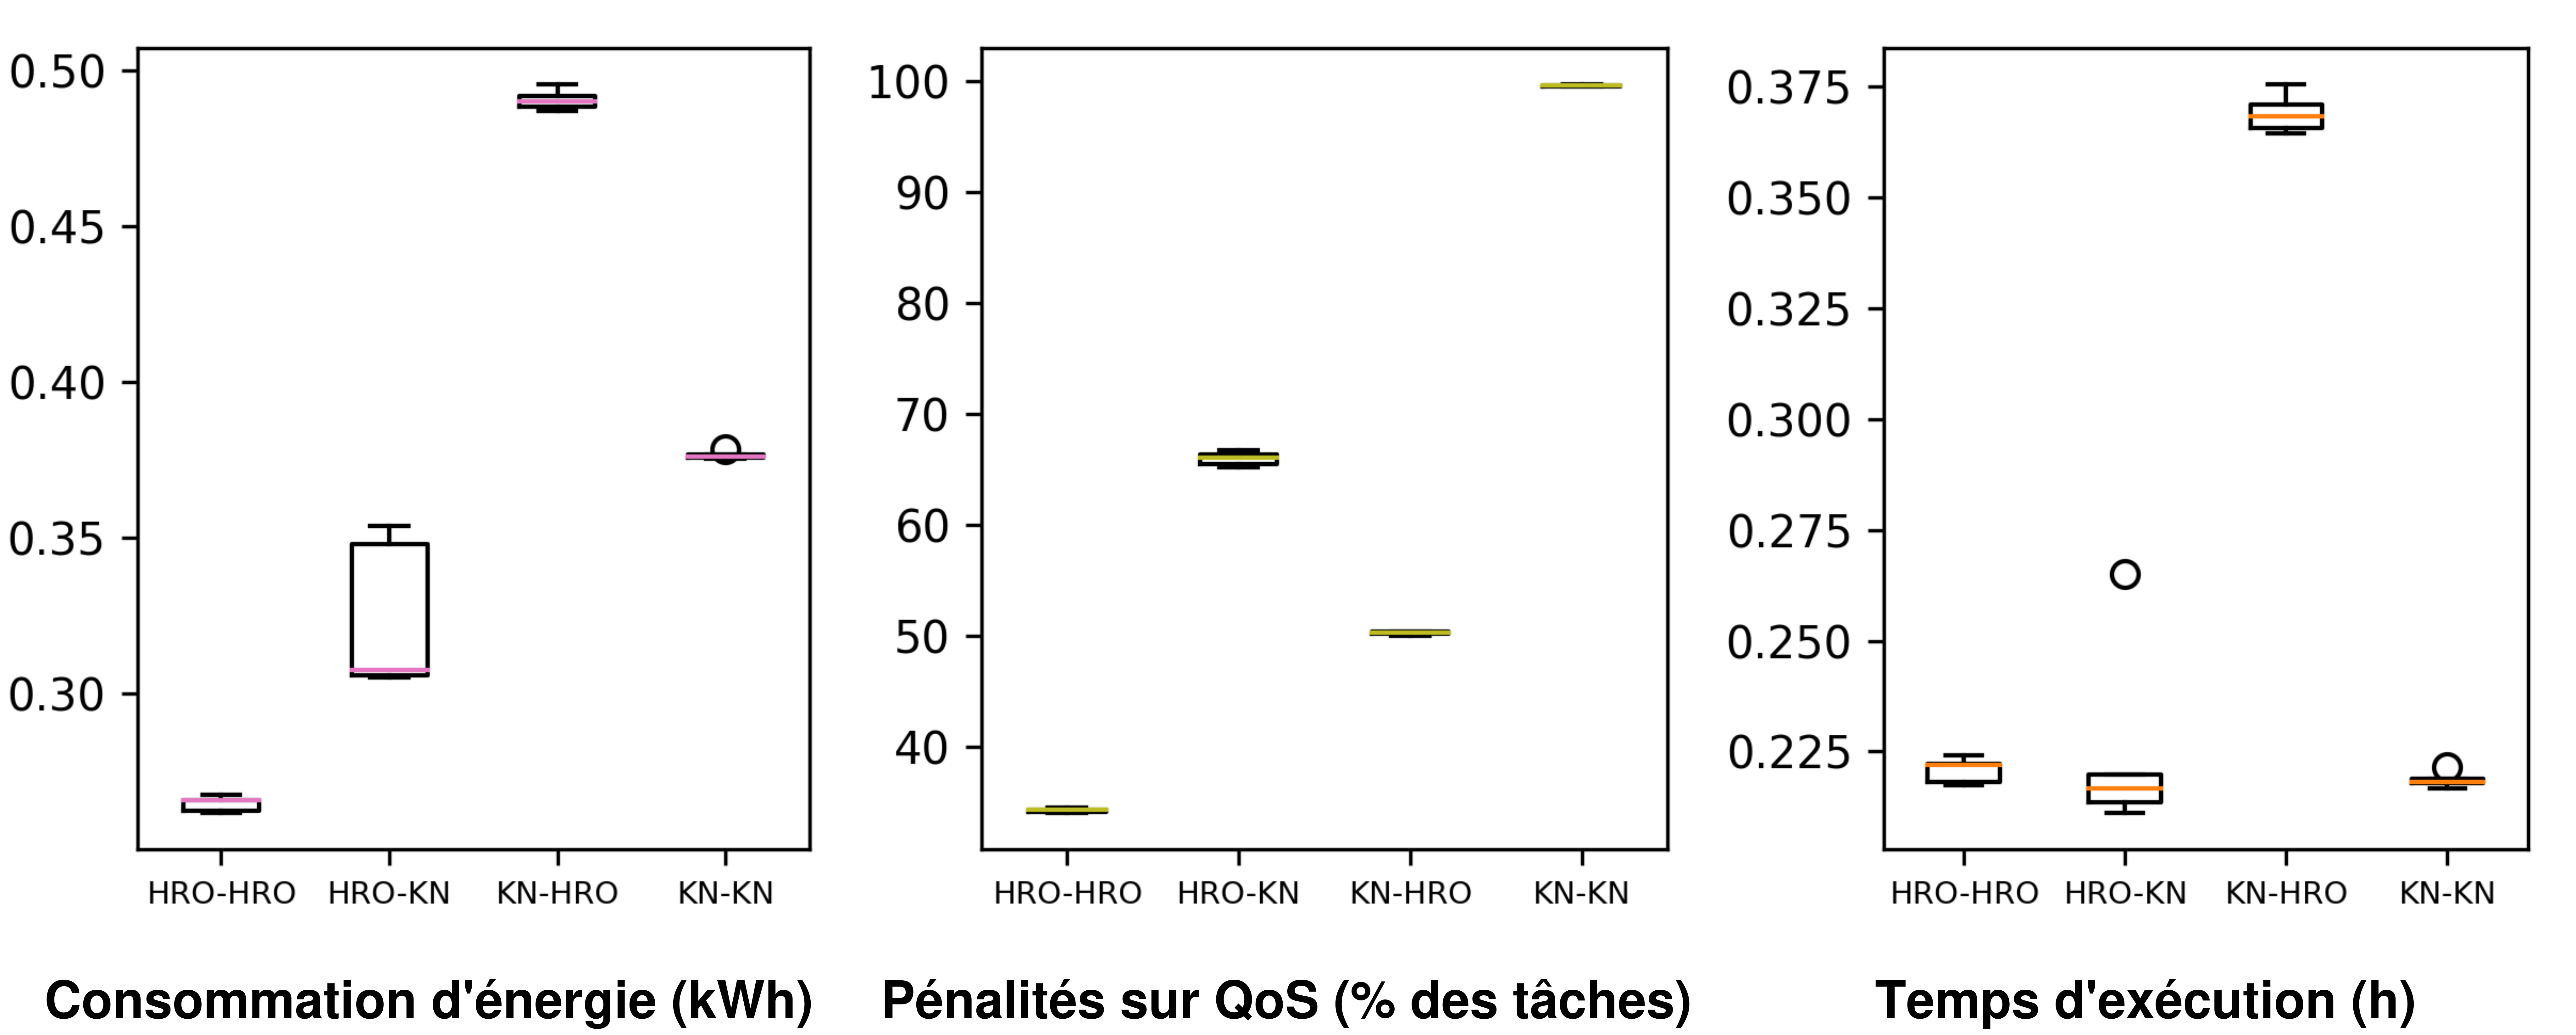
\includegraphics[width=\columnwidth]{img/eval-herofake/herofake-resultats-2.png}
        }}
    \end{center}
\end{frame}

\note[enumerate]{
    \item Résultat attendu : l'autoscaler HRO a un impact important sur la consommation d'énergie car il alloue des accélérateurs ;
    \item Résultat intéressant : l'ordonnanceur HRO permet de réduire de moitié les pénalités sur QoS en conjonction avec l'autoscaler Knative : marge de progression importante sous autoscaling sans conscience des coûts.
}

\begin{frame}{HeROfake -- Conclusion}
    \begin{columns}
        \column{0.7\textwidth}
        \begin{itemize}
            \item L'orchestrateur HeROfake donne un \textit{makespan} comparable à Knative, mais :
            \begin{itemize}
                \item Réduit les \textbf{pénalités sur QoS} de \textbf{65\%} ;
                \item \textbf{Consolide} les tâches sur \textbf{30\%} des nœuds de l'infrastructure ;
                \item Réduit la consommation d'\textbf{énergie dynamique} de plus de \textbf{35\%}.
            \end{itemize}

            \item L'approche de l'orchestration par les coûts offre une alternative aux stratégies de référence :
            \begin{itemize}
                \item Notre ordonnanceur seul permet de \textbf{diminuer de moitié} les violations de QoS en allouant uniquement des CPU.
            \end{itemize}

            \item Publication à la conférence \textit{CCGrid'23} :
            \begin{itemize}
                \item \fullcite{herofake}
            \end{itemize}
        \end{itemize}

        \column{0.3\textwidth}
        \begin{center}
            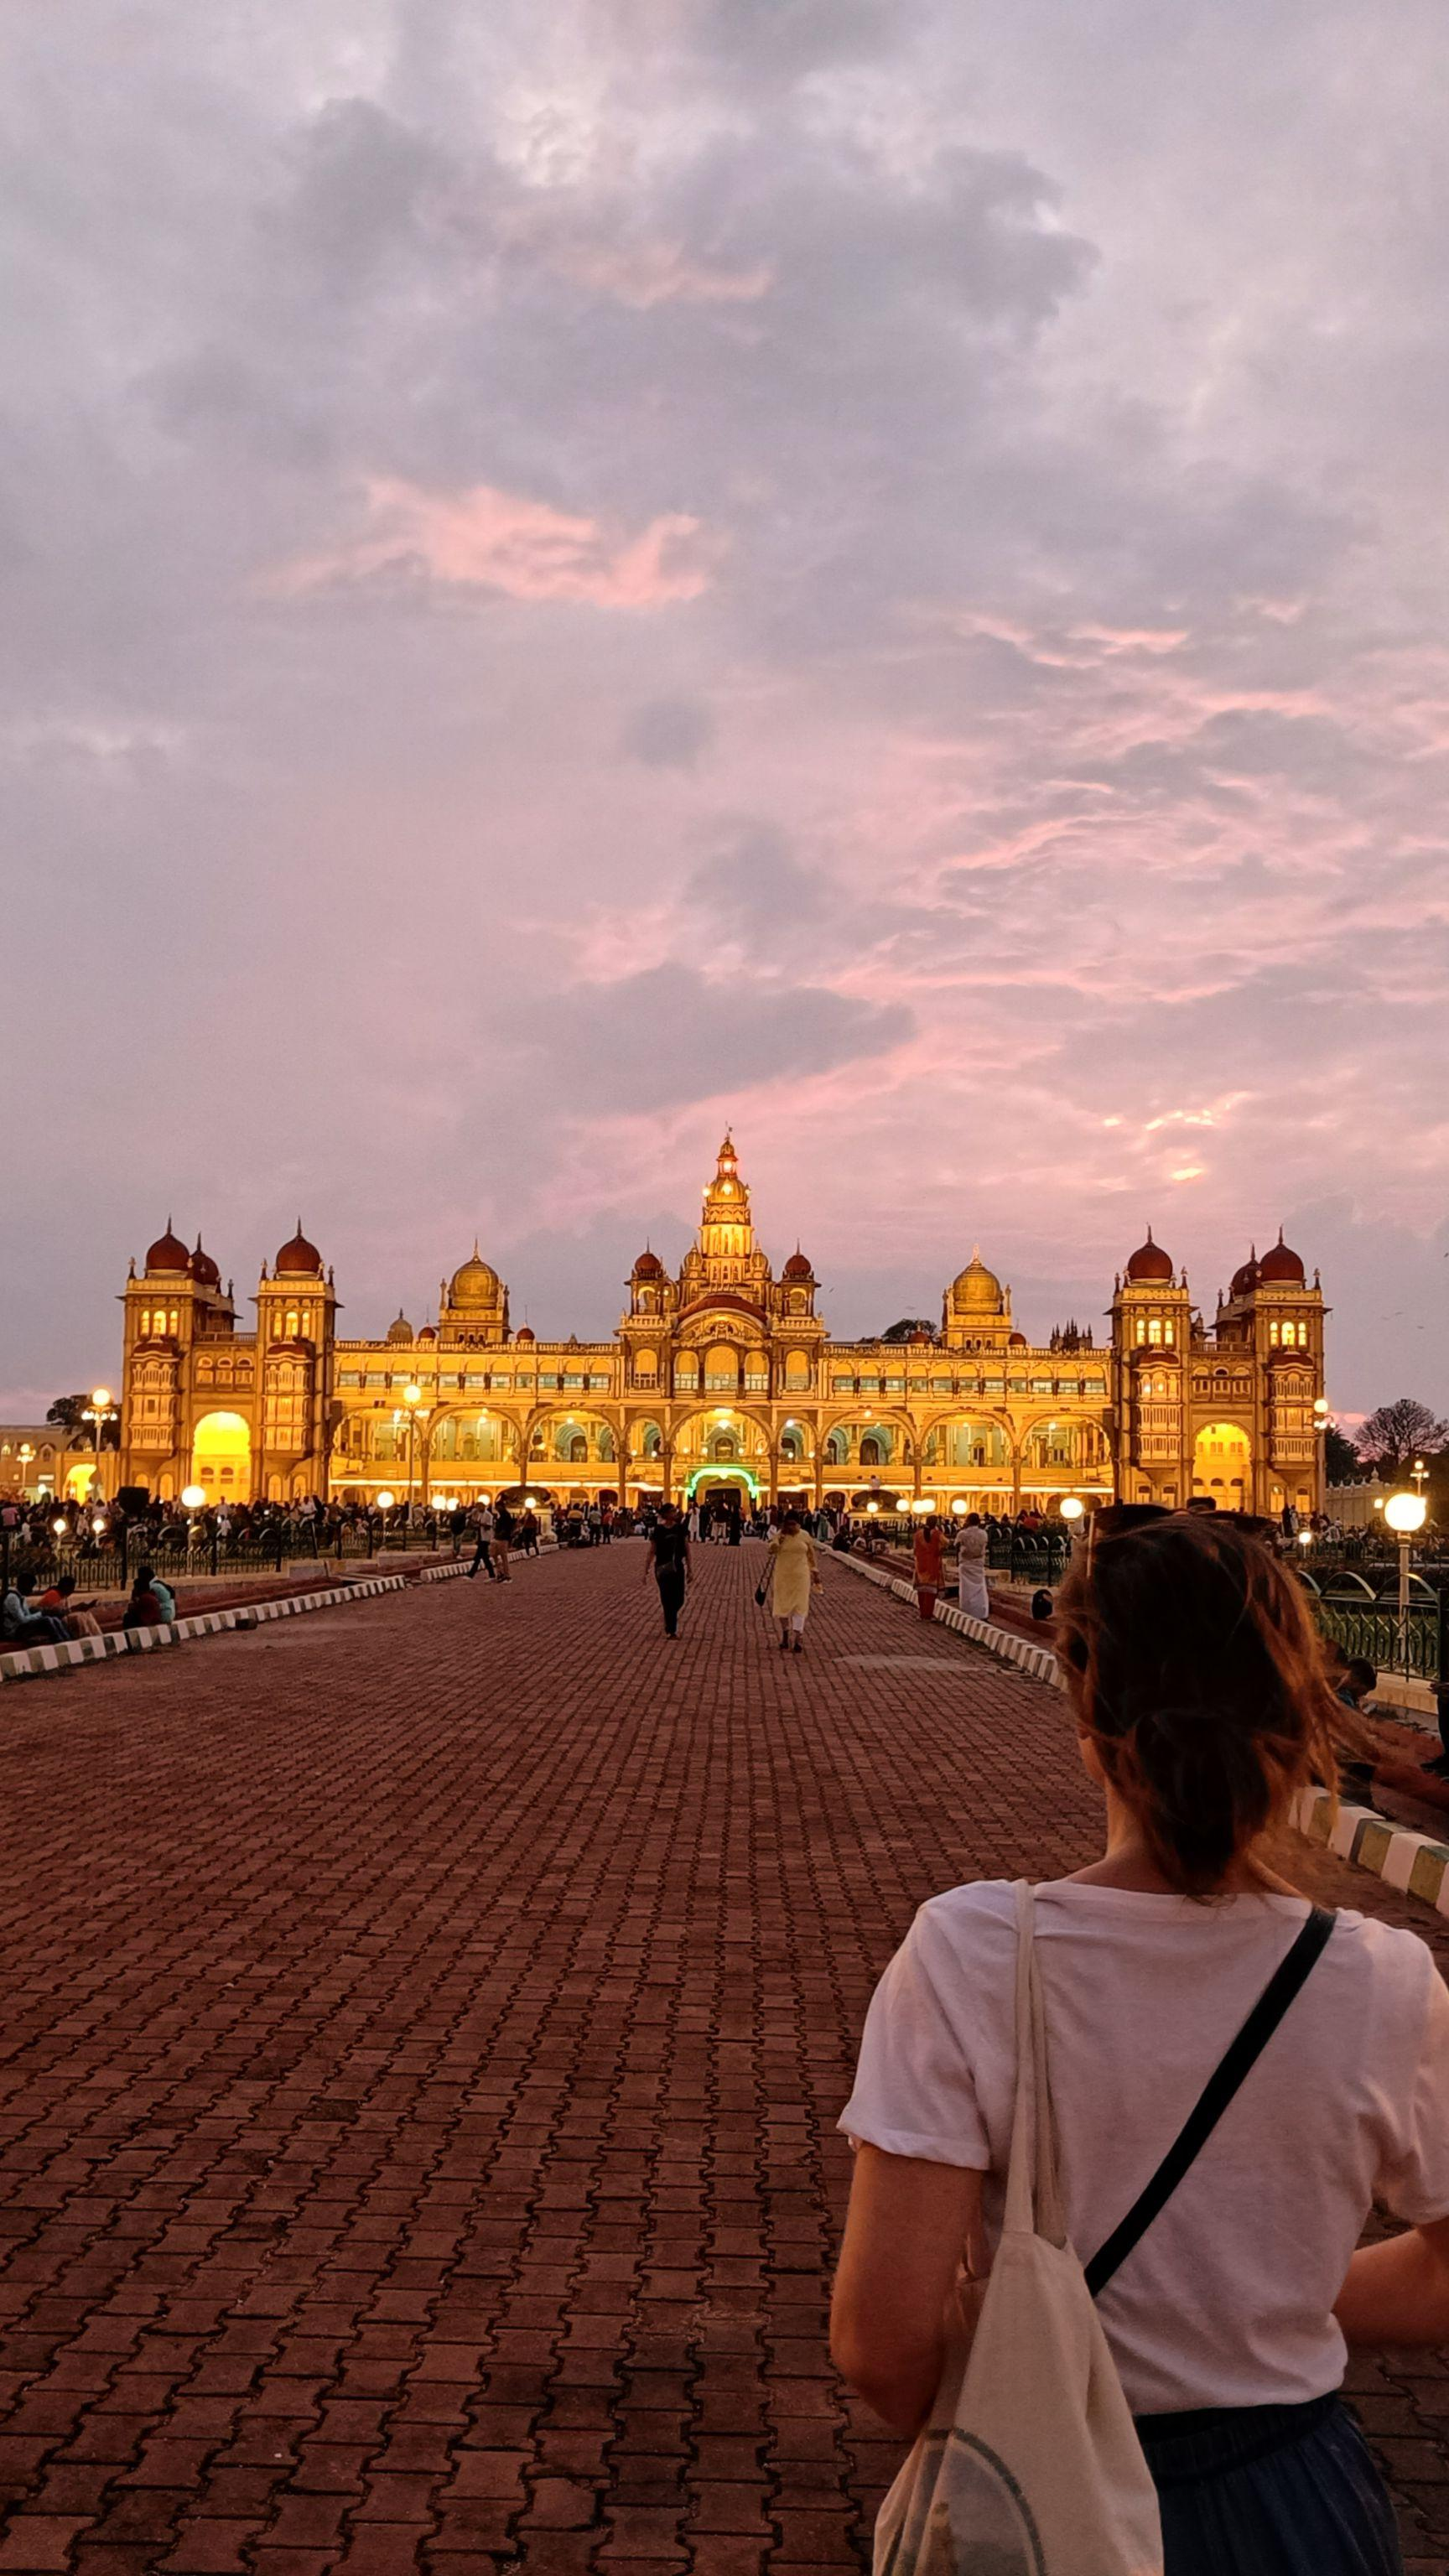
\includegraphics[width=0.9\columnwidth]{img/mysore.jpg}
        \end{center}
    \end{columns}
\end{frame}

\section{\textbf{HeROcache} -- Applications serverless et coûts associés aux systèmes de stockage}

\begin{frame}{HeROcache -- Cas d'usage}
    \begin{columns}
        \column{0.5\textwidth}
        \resizebox{0.9\columnwidth}{!}{\vbox{
            \textbf{Projet AID DISPEED : Systèmes de détection d'intrusion}
            \begin{itemize}
                \item Utilisation intermittente de ressources contraintes :
                \begin{itemize}
                    \item IDS déployés à l'edge, dans le cadre de missions pour des drones de surface ;
                \end{itemize}
                \item Les IDS reposent sur l'apprentissage automatique :
                \begin{itemize}
                    \item Random Forests, réseaux de neurones ;
                    \item Accélération matérielle.
                \end{itemize}
            \end{itemize}
    
            \textbf{Défis à relever}
            \begin{itemize}
                \item Ordonnancer des chaînes de fonctions ;
                \item Communication de résultats intermédiaires ;
                \item Images de fonctions lourdes (plusieurs Go) ;
                \item Temps d'exécution très courts (millisecondes).
            \end{itemize}
        }}

        \column{0.5\textwidth}
        \begin{center}
            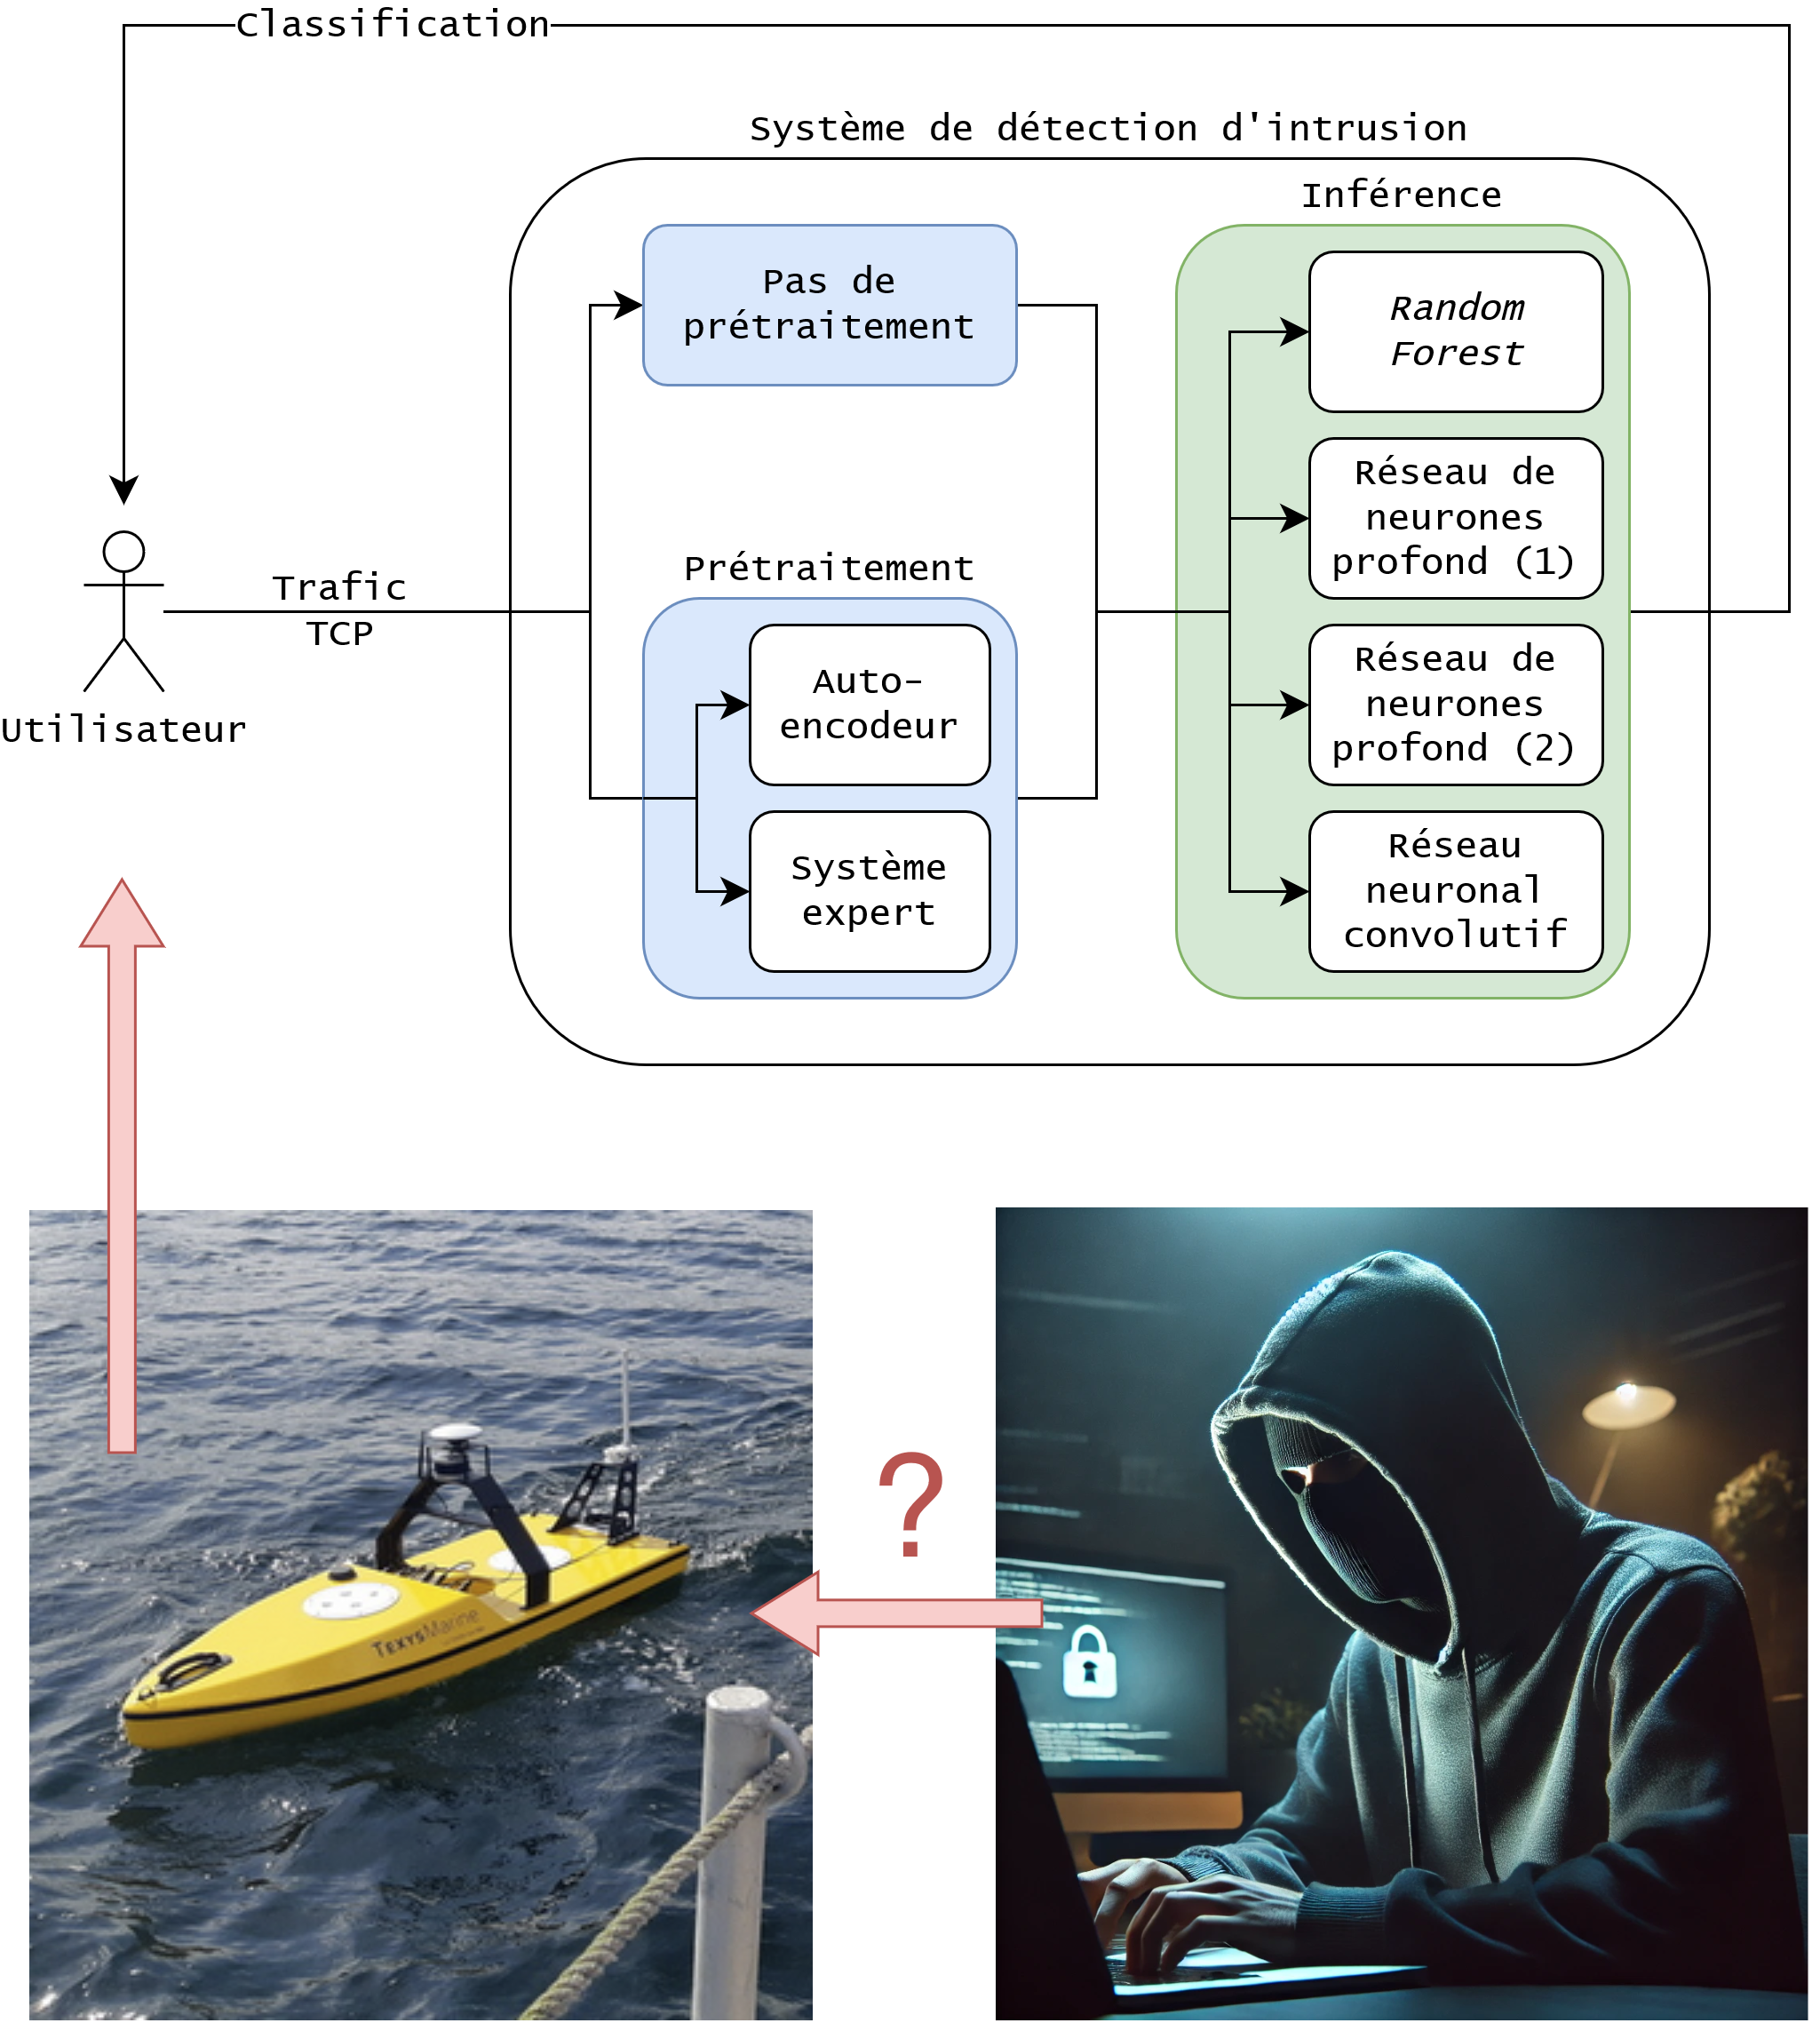
\includegraphics[width=0.8\columnwidth]{img/herocache-use-case.png}
            \footnotetext{\textbf{DISPEED} : Détection d’Intrusion et compromis Sécurité/Performance/Énergie, Étude pour les meutes de Drones}
        \end{center}
    \end{columns}
\end{frame}

\note[enumerate]{
    \item Drones de surface : part importante du calcul dans la consommation d'énergie
}

\begin{frame}{HeROcache -- Problème}
    \begin{exampleblock}{Question de recherche 2 (\textbf{QR2})}
        Comment déployer des \textbf{applications complexes}, composées de chaînes de fonctions de \textbf{courte durée}, et comment tirer parti de l'\textbf{hétérogénéité} des nœuds disponibles à l'edge, pour respecter la \textbf{qualité de service} requise par les utilisateurs tout en contenant la \textbf{consommation d'énergie} de l'infrastructure ?
    \end{exampleblock}
\end{frame}

\begin{frame}{HeROcache -- Travaux connexes}
    \begin{table}[]
        \centering
        \caption{État de l'art des plateformes d'orchestration prenant en compte les données.}
        \resizebox{\textwidth}{!}{
            \begin{tabular}{lYYYYYYY}
                \toprule
                & Chaînes de fonctions & QoS par requête & Hétérogénéité matérielle & Contrainte de programmation & Énergie & Cache de fonctions & Communications \\
                \cmidrule(lr){2-2}\cmidrule(lr){3-3}\cmidrule(lr){4-4}\cmidrule(lr){5-5}\cmidrule(lr){6-6}\cmidrule(lr){7-7}\cmidrule(lr){8-8}
                Cypress~\cite{bhasiCypressInputSizesensitive2022} & \cmark & \cmark & \xmark & \cmark & \cmark & \xmark & \cmark \\
                FaDO~\cite{smithFaDOFaaSFunctions2022} & \xmark & \xmark & \xmark & \cmark & \xmark & \xmark & \cmark \\
                FaasFlow~\cite{zijunFassflowEfficient2022} & \cmark & \xmark& \xmark & \xmark & \xmark & \xmark & \xmark \\
                FIRST~\cite{zhangFIRSTExploitingMultiDimensional2023} & \xmark & \xmark & \xmark & \cmark & \cmark & \xmark & \xmark \\
                HeROfake~\cite{herofake} & \xmark & \cmark & \cmark & \cmark & \cmark & \xmark & \xmark \\
                Netherite~\cite{burckhardtNetheriteEfficientExecution} & \cmark & \xmark & \xmark & \cmark & \xmark & \xmark & \cmark \\
                Palette~\cite{abdiPaletteLoadBalancing2023} & \cmark & \xmark & \xmark & \xmark & \xmark & \cmark & \cmark \\
                \textbf{Solution cible} & \cmark & \cmark & \cmark & \cmark & \cmark & \cmark & \cmark \\
                \bottomrule
            \end{tabular}
        }
        \label{table:herocache-sota}
    \end{table}
\end{frame}

\begin{frame}{HeROcache -- Système considéré}
    \begin{center}
        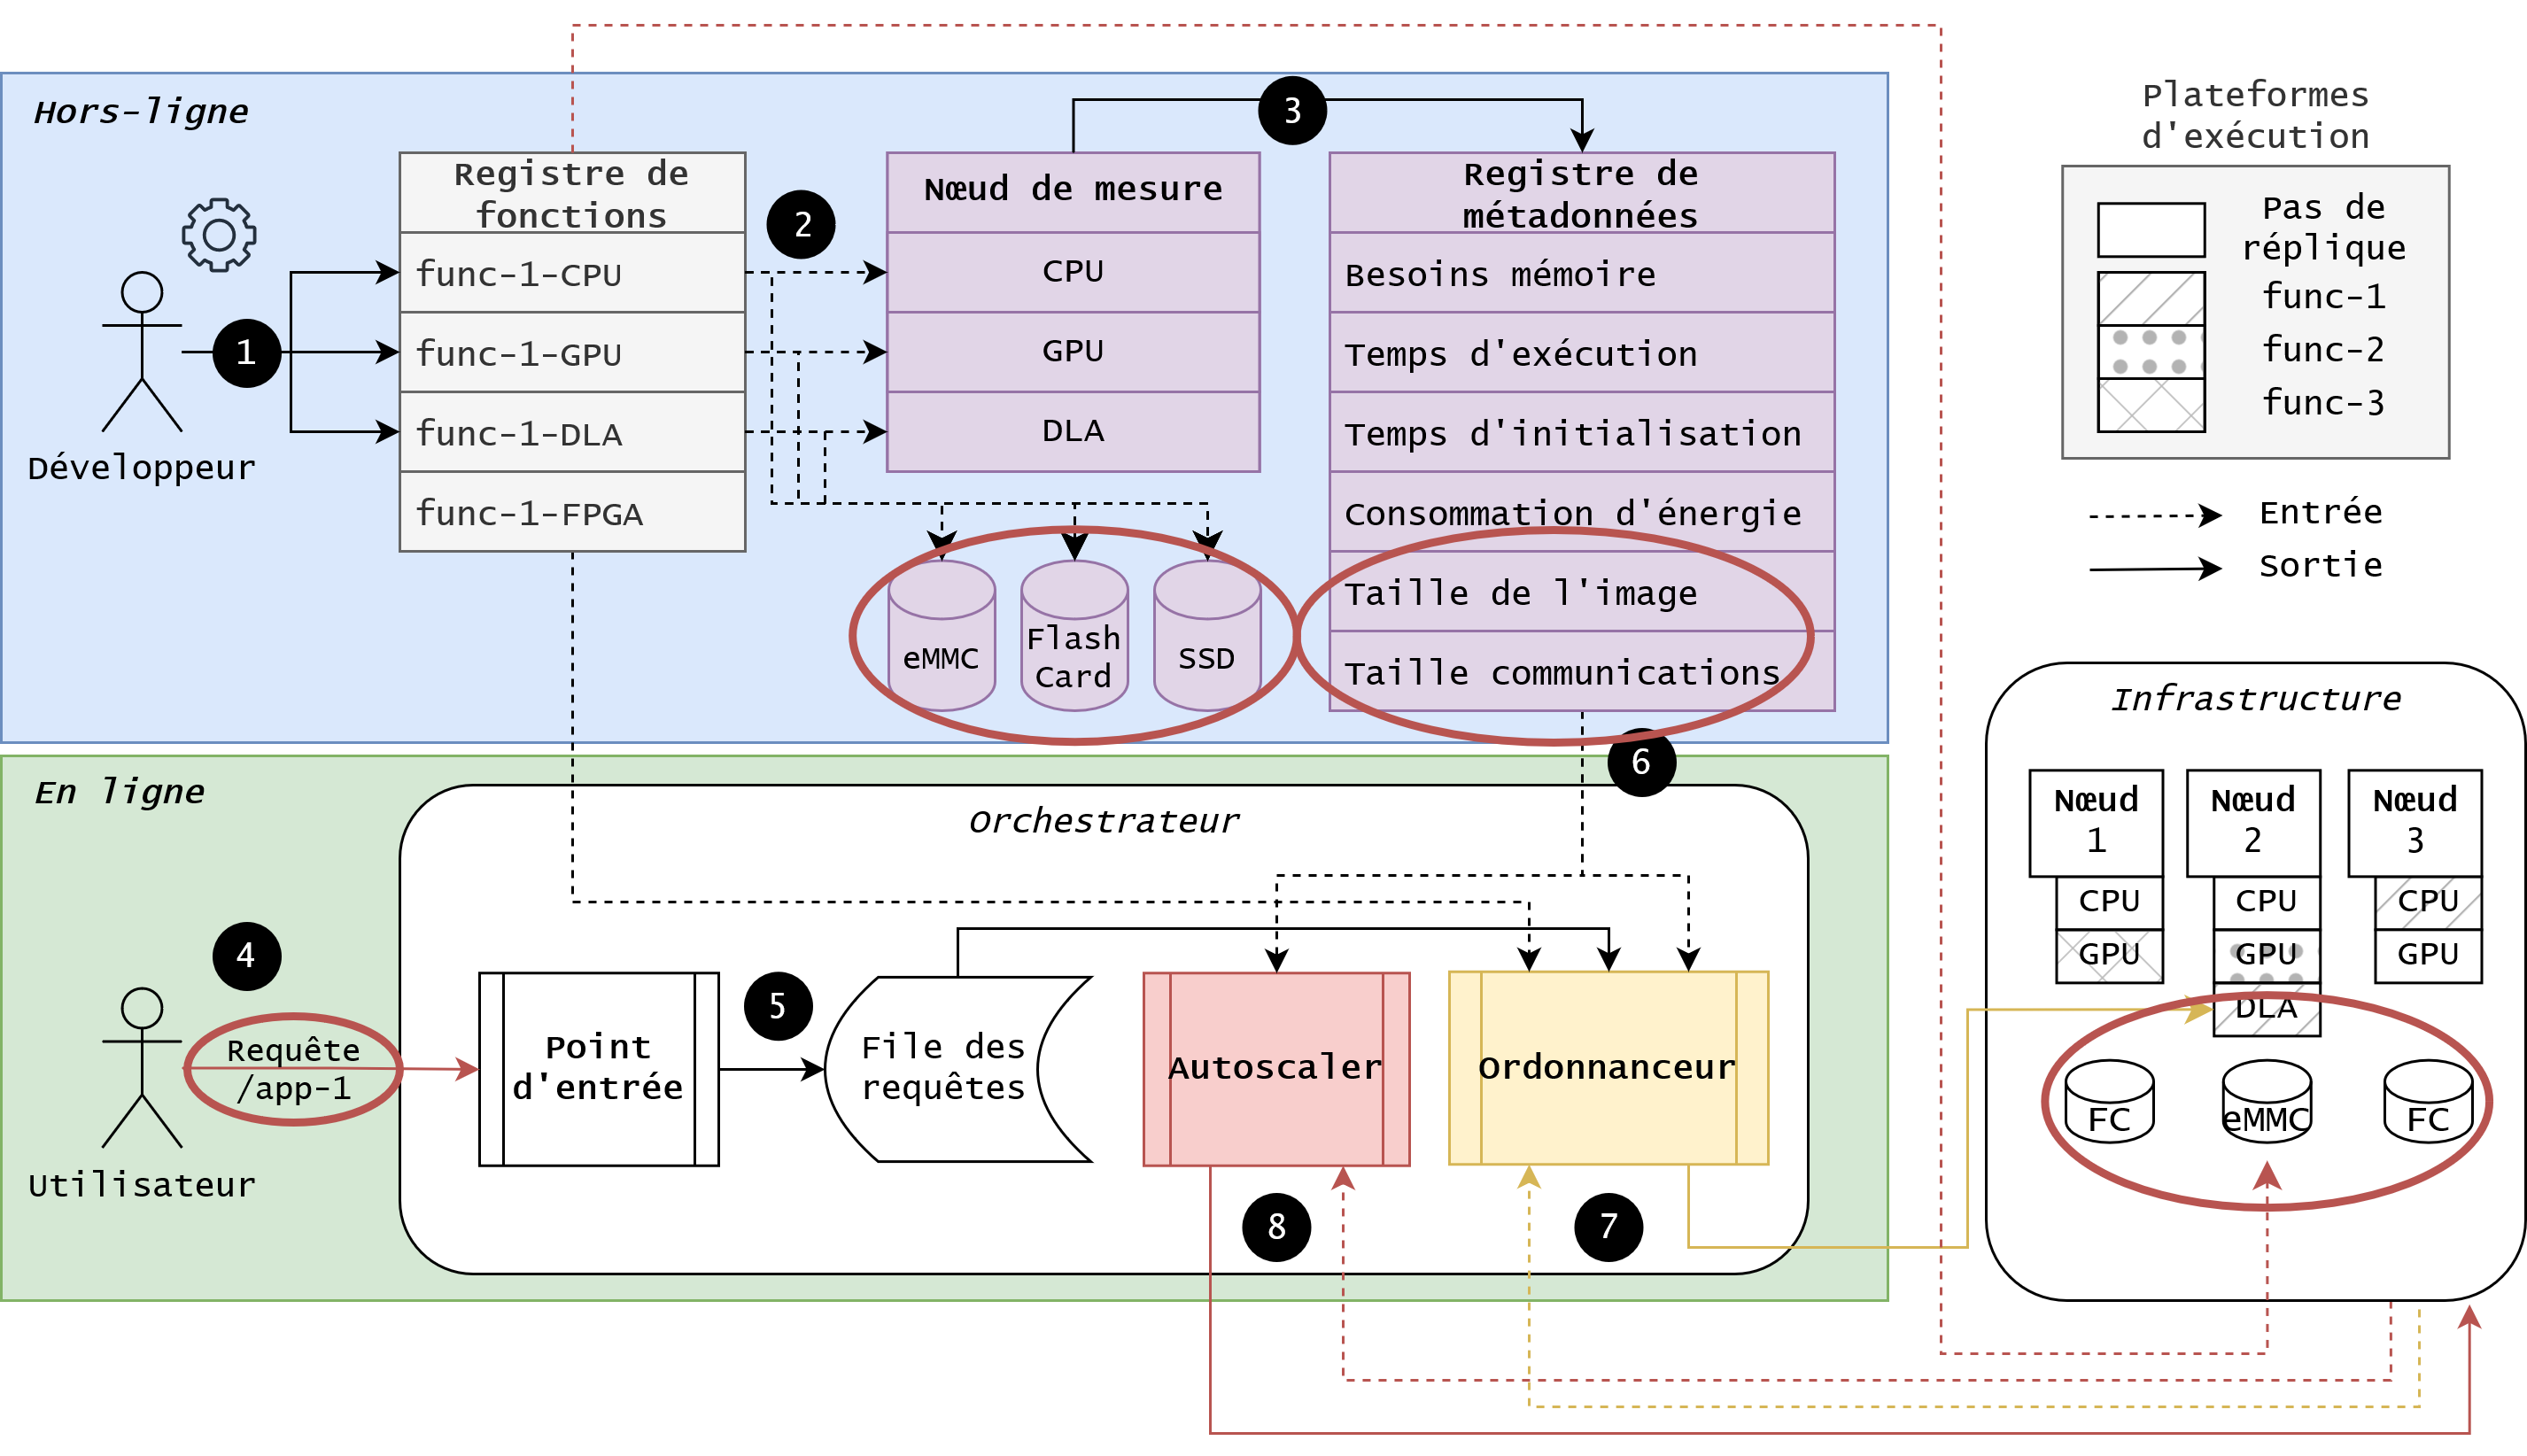
\includegraphics[width=0.8\columnwidth]{img/herocache-plateforme.png}
    \end{center}    
\end{frame}

\begin{frame}[t]{HeROcache -- Contribution : Cache et communications}
    \begin{columns}
        \column{0.5\textwidth}
        \begin{center}
            \uncovergraphics<1->[width=\columnwidth]{img/function-cache.png}

            {\small Mise en cache des images de fonctions sur les nœuds pour accélérer les démarrages à froid}
            \pause
        \end{center}

        \column{0.5\textwidth}
        \begin{center}
            \uncovergraphics<2->[width=0.8\columnwidth]{img/function-communications.png}

            {\small Consolidation des fonctions d'une même application pour favoriser les communications locales}
            \pause
        \end{center}
    \end{columns}

    \begin{center}
        \uncovergraphics<3->[width=0.8\textwidth]{img/brace.png}

        Éviter la contention sur le stockage local aux nœuds
    \end{center}
\end{frame}

\note[enumerate]{
    \item 25\% des fonctions déployées sur Microsoft Azure Functions s'exécutent en moins de 100 ms
    \item La récupération des images de fonctions peut compter jusqu'à 80\% du temps de réponse total
    \item Les communications par stockage distant peuvent ralentir l'exécution des fonctions d'un facteur 11
}

\begin{frame}{HeROcache -- Contribution : Stratégie de minimisation des coûts}
    \begin{columns}
        \column{0.55\textwidth}
        \resizebox{0.9\columnwidth}{!}{\vbox{
        \begin{itemize}
            \item \textbf{Autoscaling}
            \begin{itemize}
                \item \textbf{Minimiser} les \textcolor{blue}{défauts de cache}, la consommation d'\textcolor{orange}{énergie} et le coût de \textcolor{purple}{possession} total :
            \end{itemize}

            \resizebox{0.85\columnwidth}{!}{\vbox{
                \begin{center}
                    \begin{equation*}
                        \begin{split}
                            \forall N, \forall P \in N, \, &scaleCost^{{f}_{{i}_{N, P}}}_{a} = \\
                              &k_{CP} \cdot \textcolor{blue}{{CP}_{{a}_{N}}}
                            + k_{TT} \cdot {TT}_{{f}_{N, P}} \\
                            + &k_{EC} \cdot \textcolor{orange}{{EC}_{{f}_{N, P}}}
                            + k_{HP} \cdot \textcolor{purple}{{HP}_{{f}_{N, P}}}
                        \end{split}
                    \end{equation*}
                \end{center}
            }}

            \item \textbf{Ordonnancement}
            \begin{itemize}
                \item \textbf{Minimiser} les \textcolor{red}{pénalités} sur QoS, la consommation d'\textcolor{orange}{énergie} et la \textcolor{teal}{dispersion} des tâches :
            \end{itemize}

            \resizebox{0.85\columnwidth}{!}{\vbox{
                \begin{center}        
                    \begin{equation*}
                        \begin{split}
                            \forall (N, P) \in R_{f}, \, &schedCost_{{f}_{{i}_{N, P}}} = \\
                              &k_{QP} \cdot \textcolor{red}{{QP}_{{f}_{N, P}}} \\
                            + &k_{EC} \cdot \textcolor{orange}{{EC}_{{f}_{N, P}}} \\
                            + &k_{TC} \cdot \textcolor{teal}{{TC}_{{f}_{N, P}}}
                        \end{split}
                    \end{equation*}
                \end{center}
            }}
        \end{itemize}
        }}

        \column{0.45\textwidth}
        Mobiliser les métadonnées issues de la phase de caractérisation :

        \begin{center}
            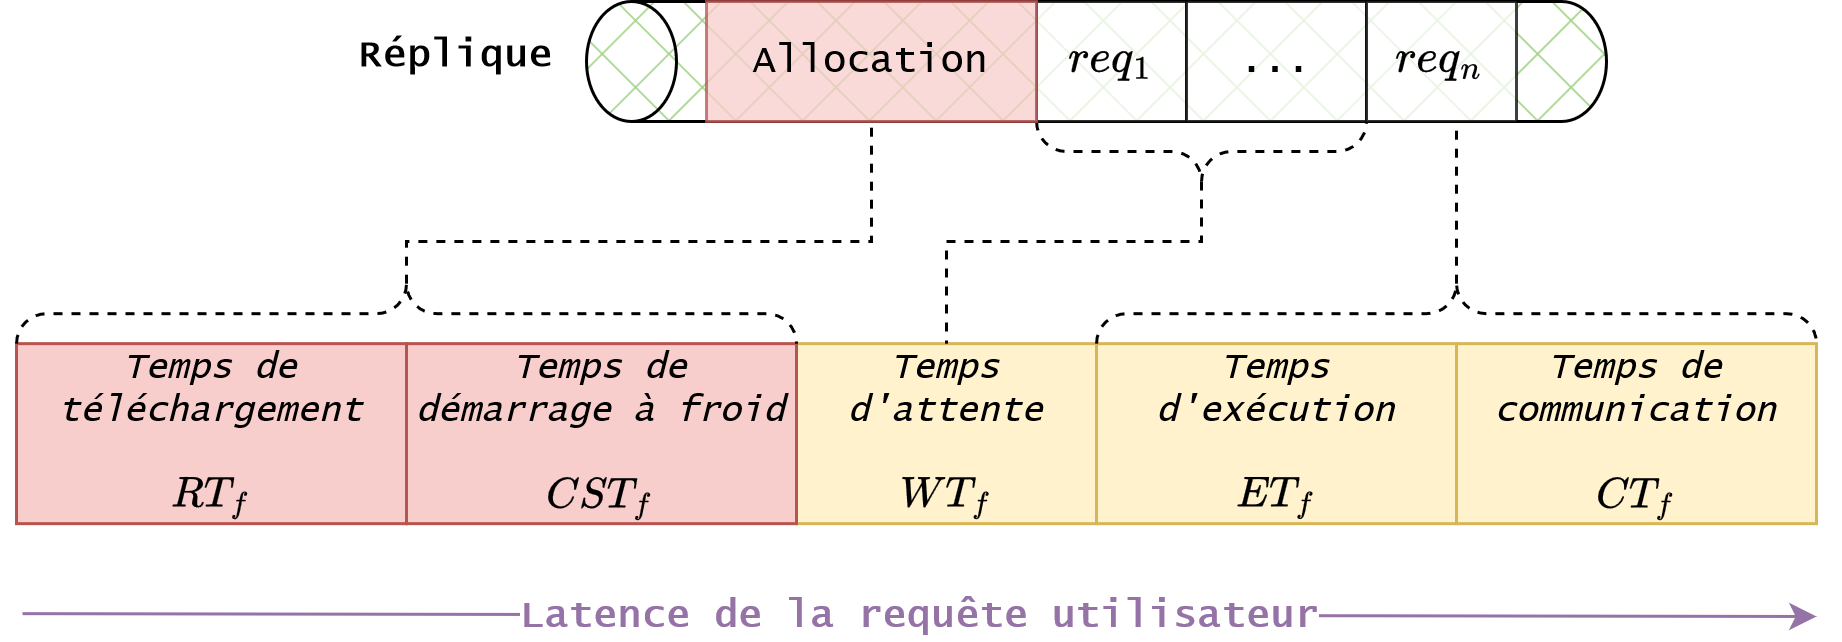
\includegraphics[width=\columnwidth]{img/herocache-total-time.png}
        \end{center}

        \begin{equation*}
            {TT}_{{f}_{N, P}} = \textcolor{blue}{{RT}_{{f}_{N, P}}} + {WT}_{{f}_{N, P}} + {CST}_{{f}_{N, P}} + {ET}_{{f}_{N, P}} + {CT}_{{f}_{N, P}}
        \end{equation*}
    \end{columns}
\end{frame}

\note[enumerate]{
    \item Autoscaler : ajout du pré-chargement en cache local des images des fonctions dans le DAG de l'application ;
    \item Scheduler : calcul des échéances en fonction de la position de la requête dans la chaîne de fonctions de l'application ;
    \item Les coefficients $k$ sont configurables par le fournisseur de services, pour donner un poids différent à chacune des composantes du coût en fonction de ses contraintes propres.
}

\begin{framefont}{\footnotesize}
\begin{frame}[t]{HeROcache -- Évaluation : Méthodologie}
    \begin{columns}
        \column[t]{0.5\textwidth}
        Politiques évaluées pour la \textbf{mise à l'échelle} :

        \begin{itemize}
            \item HeROcache (\textbf{HRC}) -- Autoscaler conscient des coûts de stockage (images de fonctions, communications entre fonctions) ;
            \item HeROfake (\textbf{HRO}) -- Autoscaler sans conscience des coûts du stockage ;
            \item Knative (\textbf{KN}) -- Équilibrage de charge.
        \end{itemize}

        \textbf{Infrastructure retenue} :
        \begin{itemize}
            \item 10 nœuds edge : 8x Raspberry Pi 4B, 1x Nvidia Jetson Xavier AGX, 1x PYNQ-Z2 (\textit{System on Chip} avec FPGA).
        \end{itemize}

        \textbf{Scénario d'évaluation} :
        \begin{itemize}
            \item Processus de Poisson, $\lambda = 83$ (12,5~Mo/s, 4G LTE) ;
            \item 10 minutes de requêtes utilisateur.
        \end{itemize}

        \column[t]{0.5\textwidth}
        Politiques évaluées pour l'\textbf{ordonnancement} :

        \begin{itemize}
            \item HeROcache (\textbf{HRC}) -- Ordonnanceur conscient des dépendances entre les tâches ;
            \item HeROfake (\textbf{HRO}) -- Ordonnanceur sans conscience des dépendances ;
            \item Knative (\textbf{KN}) -- Répliques homogènes, équilibrage de charge~\footnotemark{} ;
            \item Bin-Packing First Fit (\textbf{BPFF}) -- Ordonnanceur AWS Lambda, consolidation maximale~\footnotemark{} ;
            \item Random Placement (\textbf{RP}) -- Sélection d'une réplique aléatoire.
        \end{itemize}
    \end{columns}

    % \noindent\rule{\textwidth}{1pt}

    % \begin{columns}
    %     \column{0.5\textwidth}


    %     \column{0.5\textwidth}

    % \end{columns}

    \addtocounter{footnote}{1}
    \footnotetext{\fullcite{sureshENSUREEfficientScheduling2020}}
    \addtocounter{footnote}{1}
    \footnotetext{\fullcite{wangPeekingCurtainsServerlessb}}
\end{frame}
\end{framefont}

\begin{frame}{HeROcache -- Évaluation : Analyse des résultats}
    \begin{center}
        \resizebox{0.8\columnwidth}{!}{\vbox{
            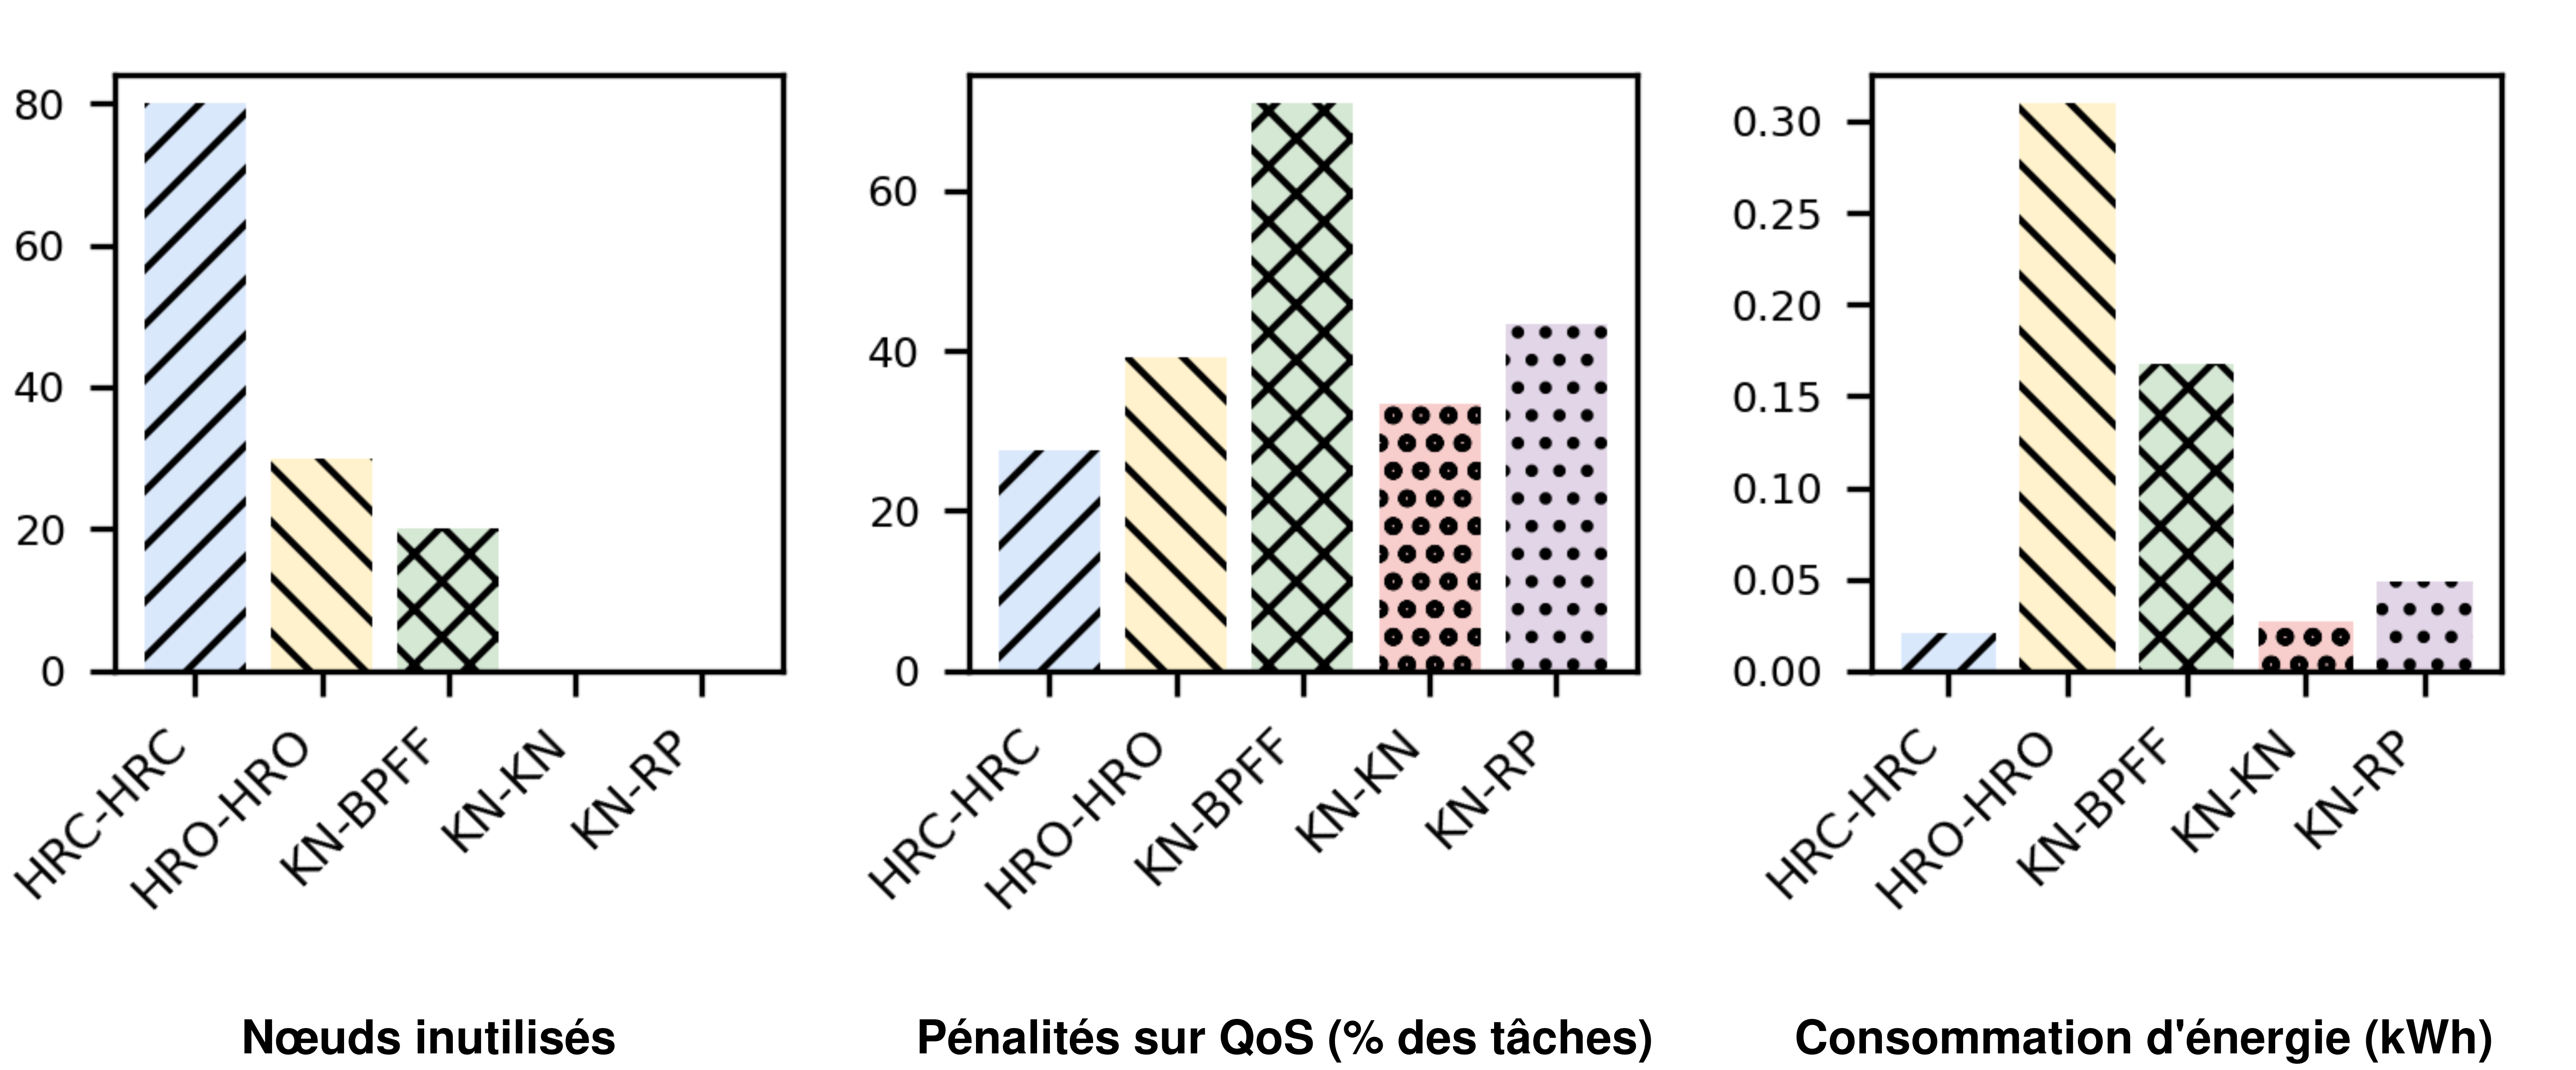
\includegraphics[width=\columnwidth]{img/eval-herocache/herocache-resultats-1.png}
        }}
    \end{center}
\end{frame}

\note[enumerate]{
    \item HeROcache permet la meilleure QoS avec la meilleure consolidation (opportunité de réduction de la conso d'énergie statique) et la meilleure consommation d'énergie dynamique (mobilisation pertinente des accélérateurs matériels) ;
    \item C'est un résultat important car les cartes edge sont faciles à éteindre et rallumer en fonction du besoin (commande à distance, traitements sans état, temps de démarrage rapides...)
    \item Knative est autorisé à allouer des accélérateurs pour ce cas d'étude. Diminue les pénalités mais en mobilisant l'intégralité de l'infrastructure !
}

\begin{frame}{HeROcache -- Évaluation : Analyse des résultats}
    \begin{center}
        \resizebox{0.8\columnwidth}{!}{\vbox{
            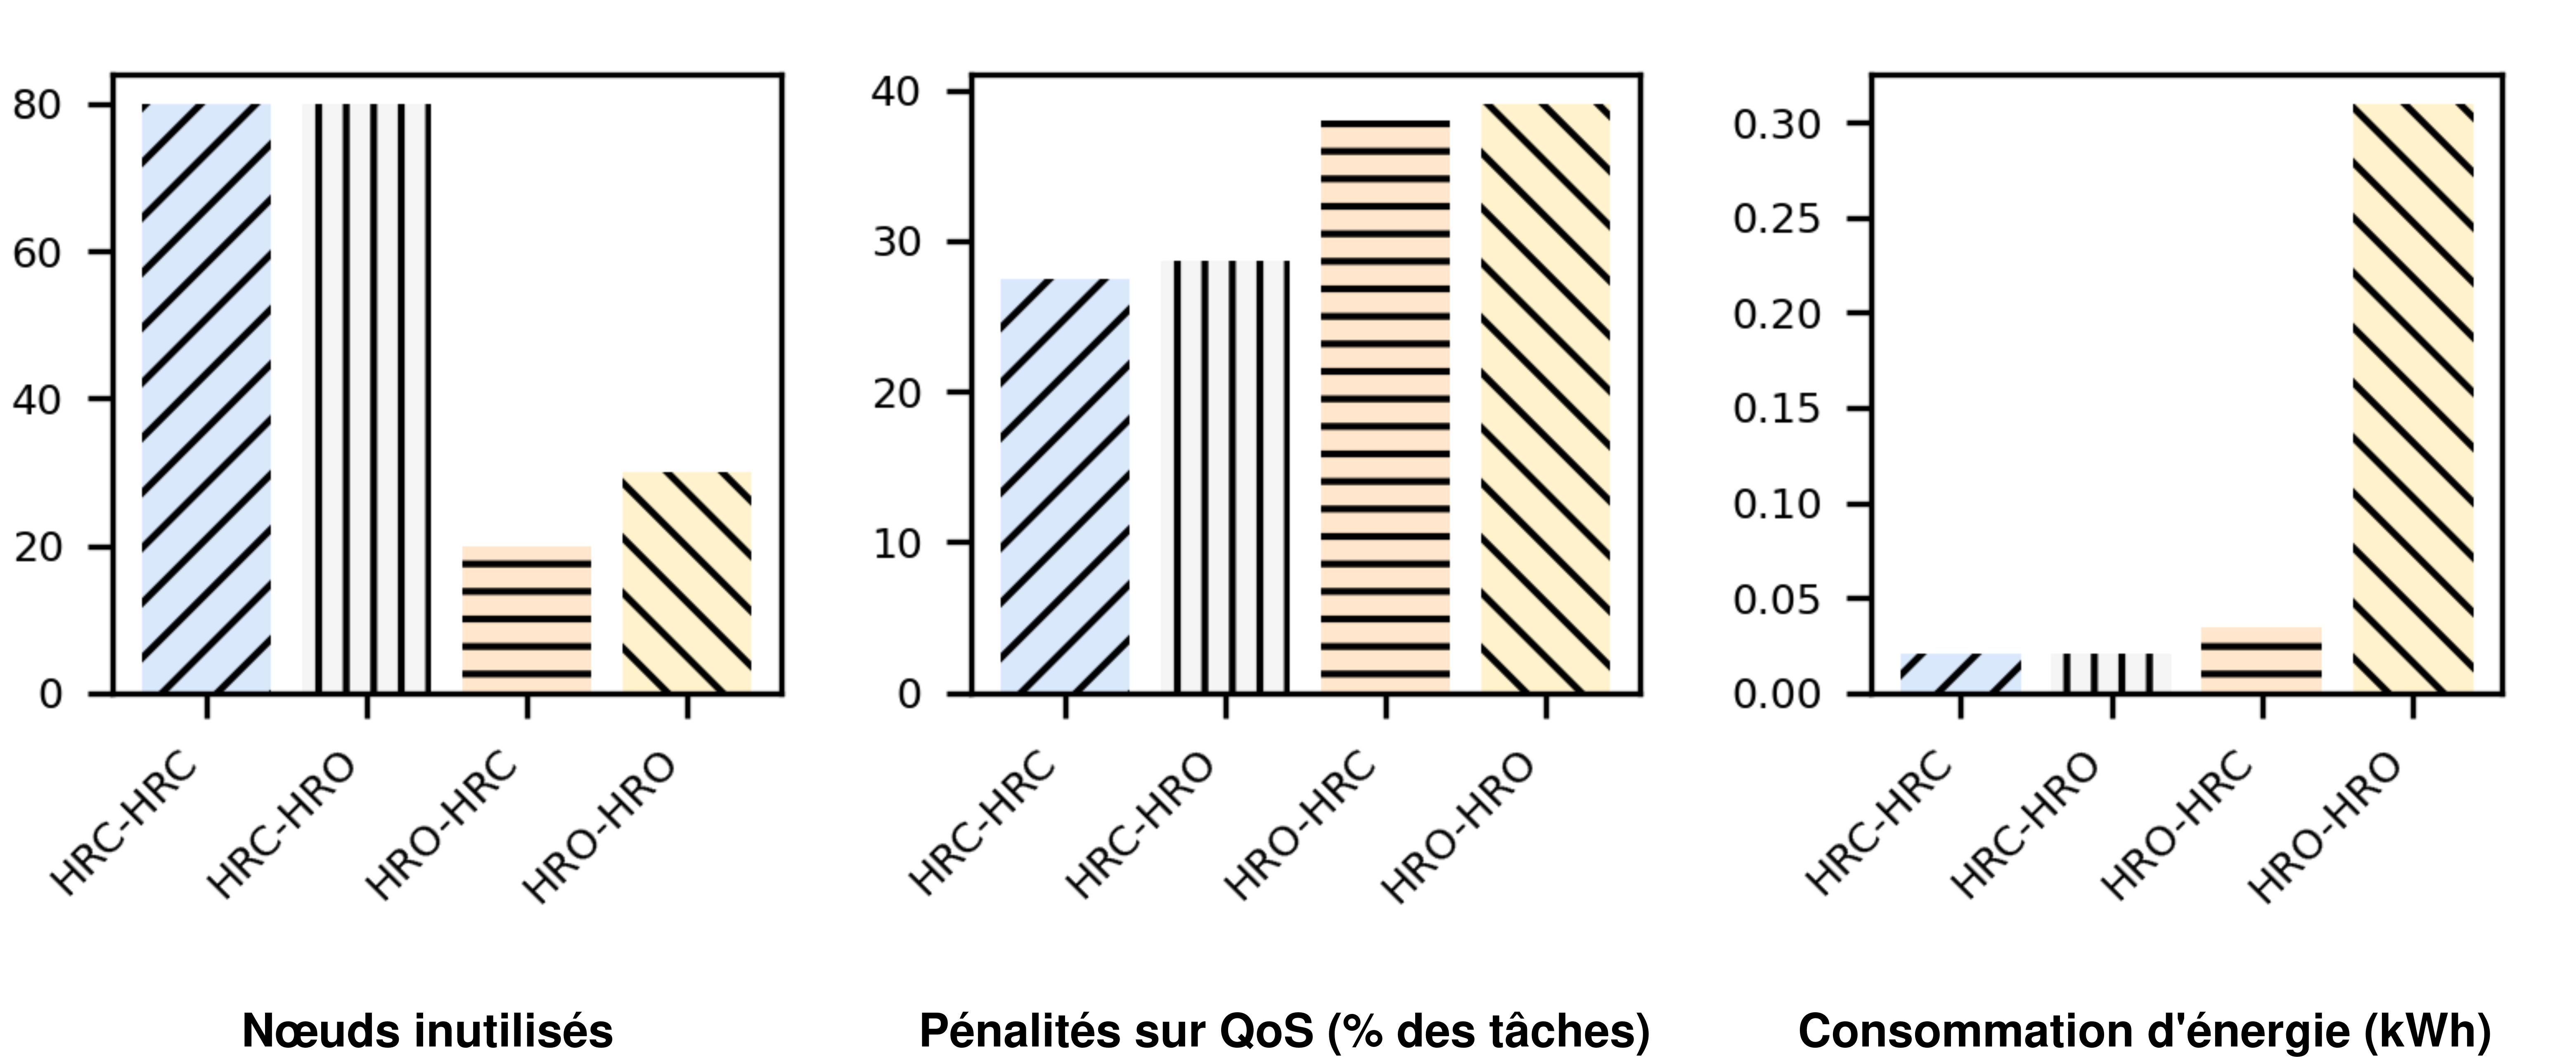
\includegraphics[width=\columnwidth]{img/eval-herocache/herocache-resultats-2.png}
        }}
    \end{center}
\end{frame}

\note[enumerate]{
    \item L'autoscaler HeROcache est le seul à permettre une bonne consolidation, car il prend en compte les dépendances pour l'allocation des répliques ;
    \item HeROfake : makespan plus long car l'ordonnanceur ne prend pas en compte les dépendances entre les tâches. Ordonnance par priorité globale plutôt que par application, tout en cherchant à consolider les tâches, ce qui provoque un fort ralentissement.
}

\begin{frame}{HeROcache -- Conclusion}
    \begin{columns}
        \column{0.7\textwidth}
        \begin{itemize}
            \item HeROcache consolide les fonctions des mêmes applications :
            \begin{itemize}
                \item réduction des délais d'\textbf{initialisation} de \textbf{17,6\%} en moyenne ;
                \item réduction des délais de \textbf{communication} de \textbf{88,4\%} ;
            \end{itemize}
            \item HeROcache améliore la Qualité de Service :
            \begin{itemize}
                \item maintien des \textbf{violations de QoS} sous les \textbf{28\%} des requêtes ;
                \item potentiel de réduction de la consommation d'\textbf{énergie statique} de \textbf{80\%}.
            \end{itemize}
            \item Publication à la conférence \textit{CCGrid'24} :
            \begin{itemize}
                \item \fullcite{herocache}
            \end{itemize}
        \end{itemize}

        \column{0.3\textwidth}
        \begin{center}
            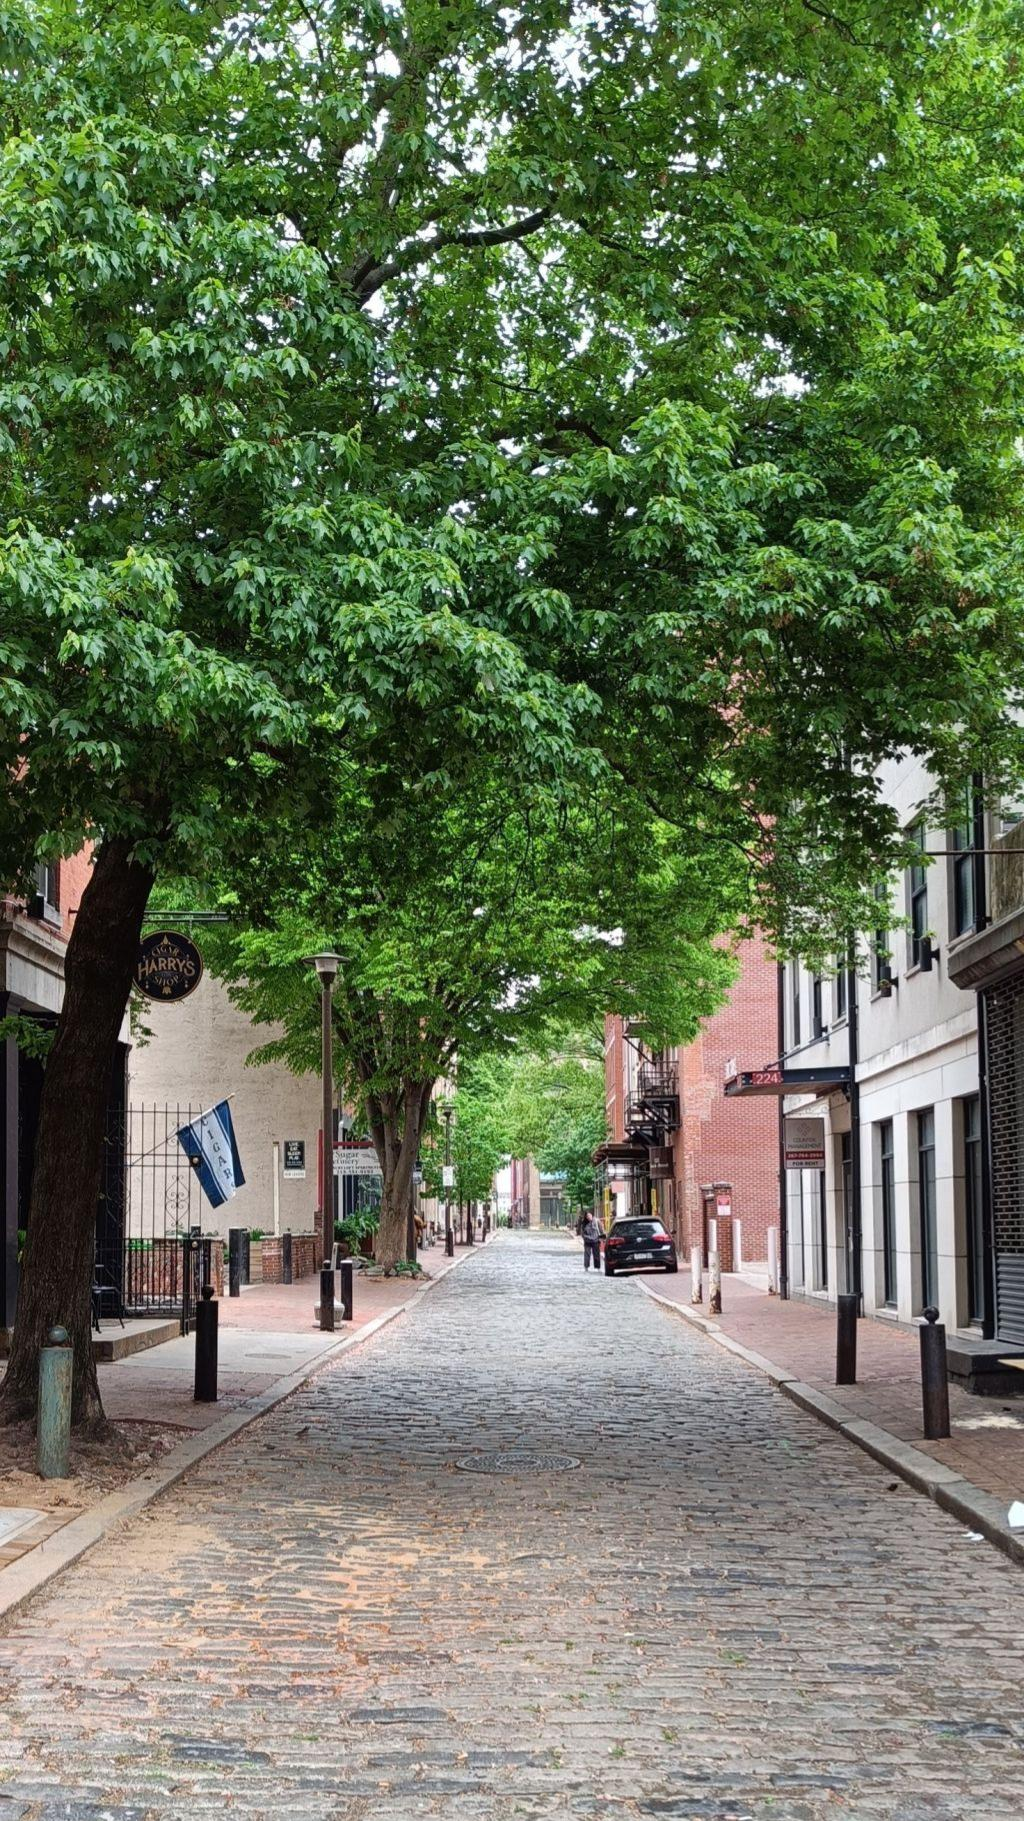
\includegraphics[width=0.9\columnwidth]{img/philly.jpg}
        \end{center}
    \end{columns}
\end{frame}

\section{\textbf{HeROsim} -- Simuler pour élaborer et évaluer des politiques d'orchestration serverless}

\begin{frame}{HeROsim -- Problème}
    \begin{exampleblock}{Question de recherche 3 (\textbf{QR3})}
        Du point de vue d'un fournisseur de services pour le cloud, comment \textbf{évaluer} et \textbf{comparer} l'impact sur la \textbf{qualité de service} de différentes \textbf{politiques} d'allocation de ressources et d'ordonnancement de tâches dans le modèle \textbf{serverless} ?
    \end{exampleblock}
\end{frame}

\begin{frame}{HeROsim -- Travaux connexes}
    \begin{table}[]
        \centering
        \caption{État de l'art des outils de simulation pour l'orchestration des ressources et des charges de travail dans le cloud.}
        \resizebox{\linewidth}{!}{
            \begin{tabular}{lYYYYYYYYY}
            \toprule
            & Serverless & Déploiements & Chaînes de fonctions & Hétérogénéité matérielle & QoS par requête & Énergie & Visualisation \\
            \cmidrule(lr){2-2}\cmidrule(lr){3-3}\cmidrule(lr){4-4}\cmidrule(lr){5-5}\cmidrule(lr){6-6}\cmidrule(lr){7-7}\cmidrule(lr){8-8}
            CloudSim~\cite{calheiros_cloudsim_2011} & \xmark & Public, privé, hybride & \xmark & \cmark & \xmark & \cmark & \xmark \\
            CloudSimSC~\cite{mampage_cloudsimsc_2023} & \cmark & Public, privé, hybride & \xmark & \cmark & \xmark & \cmark & \xmark \\
            CloudAnalyst~\cite{wickremasinghe_cloudanalyst_2010} & \xmark & Public, privé, hybride & \xmark & \cmark & \xmark & \cmark & \cmark \\
            DFaaSCloud~\cite{jeonCloudSimExtensionSimulatingDistributed2019} & \cmark & Hybride multi-strates & \xmark & \xmark & \cmark & \xmark & \cmark \\
            ElasticSim~\cite{cai_elasticsim_2017} & \xmark & Public & \cmark & \xmark & \xmark & \xmark & \cmark \\
            GridSim~\cite{buyyaGridSimToolkitModeling2002} & \xmark & Grille & \xmark & \cmark & \cmark & \xmark & \cmark \\
            iCanCloud~\cite{nunez_icancloud_2012} & \xmark & Public & \xmark & \xmark & \xmark & \xmark & \cmark \\
            iFogSim2~\cite{mahmudIFogSim2ExtendedIFogSim2021} & \xmark & Edge, Fog & \xmark & \cmark & \xmark & \cmark & \xmark \\
            OpenDC 2.0~\cite{mastenbroekOpenDCConvenientModeling2021} & \cmark & Public, privé, hybride & \cmark & \cmark & \xmark & \cmark & \cmark \\
            SimFaaS~\cite{mahmoudiSimFaaSPerformanceSimulator2021} & \cmark & Public & \xmark & \xmark & \xmark & \cmark & \cmark \\
            \textbf{Solution cible} & \cmark & Privé & \cmark & \cmark & \cmark & \cmark & \cmark \\
            \bottomrule
            \end{tabular}
        }
        \label{table:herosim-sota}
    \end{table}
\end{frame}

\begin{framefont}{\small}
\begin{frame}{HeROsim -- Contribution}
    \begin{itemize}
        \item \textbf{Granularité} : tracer les événements d'orchestration au niveau d'une requête utilisateur ;
        \item \textbf{Charges de travail} : modéliser les dépendances temporelles et de données ;
        \item \textbf{Hétérogénéité} : des ressources matérielles, des besoins en Qualité de Service ;
        \item \textbf{Reproductibilité} : rejouer des traces d'exécution ;
        \item \textbf{Explicabilité} : comparer des politiques au regard de métriques de performance.
    \end{itemize}

    \begin{center}
        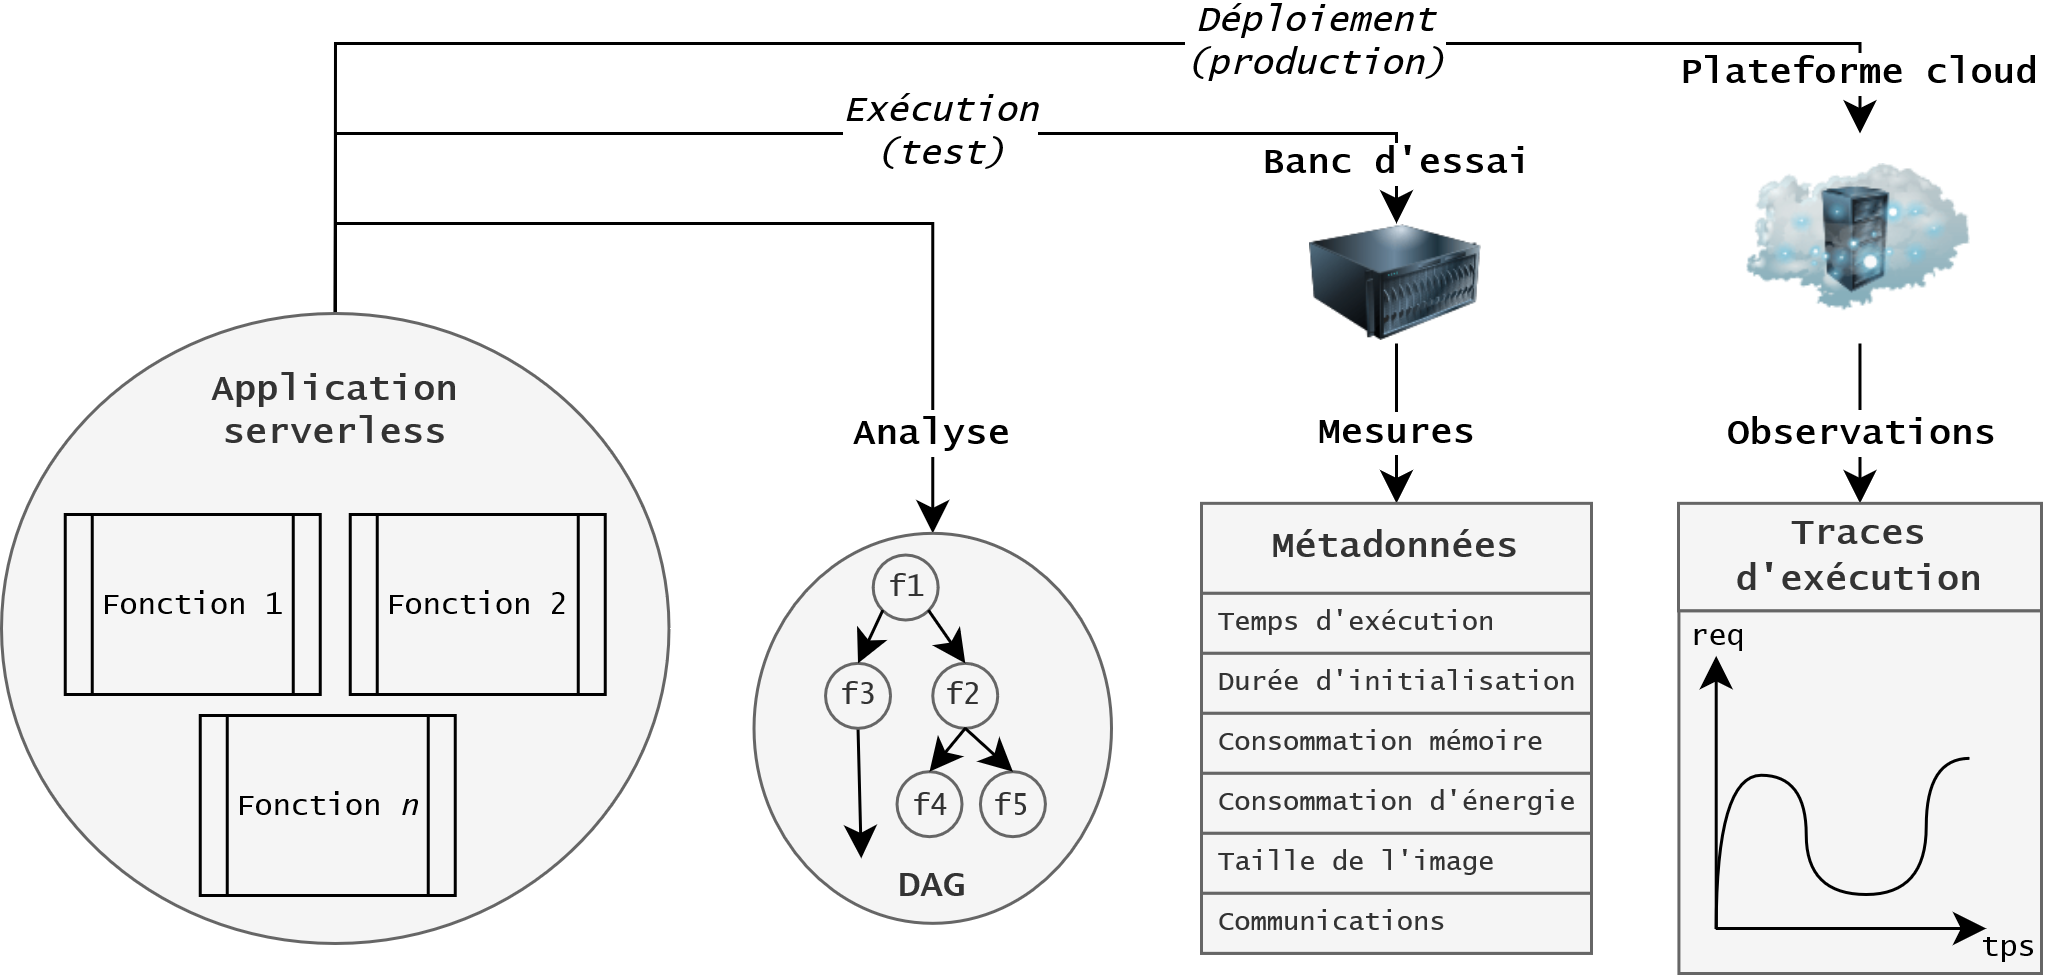
\includegraphics[width=0.6\columnwidth]{img/characterization.png}
    \end{center}
\end{frame}
\end{framefont}

\note[enumerate]{
    \item Possibilité 1 : avoir la plateforme réelle, les applications réelles, du trafic réel et mesurer les métriques de QoS
    \item Possibilité 2 : modéliser la plateforme, les applications et les utilisateurs pour simuler et rejouer des scénarios d'orchestration
    \item Méthodologie de caractérisation : mesures des fonctions (20x, moyennes), analyse des applications (DAG), générations de traces d'exécution (Poisson)
}

% \begin{frame}[fragile]{HeROsim -- Modéliser des infrastructures hétérogènes}
%     \begin{columns}
%         \column{0.3\textwidth}
%         \begin{minted}[fontsize=\footnotesize]{json}
% {
%   "network": {
%     "bandwidth": 100
%   },
%   "nodes": [
%     {
%       "memory": 8,
%       "platforms": [
%         "exampleCpu",
%         "exampleCpu"
%       ],
%       "storage": [
%         "flashCard"
%       ]
%     },
%         \end{minted}

%         \column{0.3\textwidth}
%         \begin{minted}[fontsize=\footnotesize]{json}
%     {
%       "memory": 16,
%       "platforms": [
%         "exampleCpu",
%         "exampleCpu",
%         "exampleCpu",
%         "exampleCpu"
%       ],
%       "storage": [
%       ]
%     }
%   ]
% }
%         \end{minted}
%         \column{0.3\textwidth}
%         \begin{minted}[fontsize=\footnotesize]{json}
% {
%   "flashCard": {
%     "name": "Flash Card",
%     "hardware": "flash",
%     "capacity": 64,
%     "iops": {
%       "read": 3000,
%       "write": 1000
%     },
%     "throughput": {
%       "read": 100,
%       "write": 40
%     },
%     "latency": {
%       "read": 0.001,
%       "write": 0.001
%     }
%   }
% }
%         \end{minted}
%     \end{columns}
% \end{frame}

\begin{frame}{HeROsim -- Architecture logicielle}
    \begin{center}
        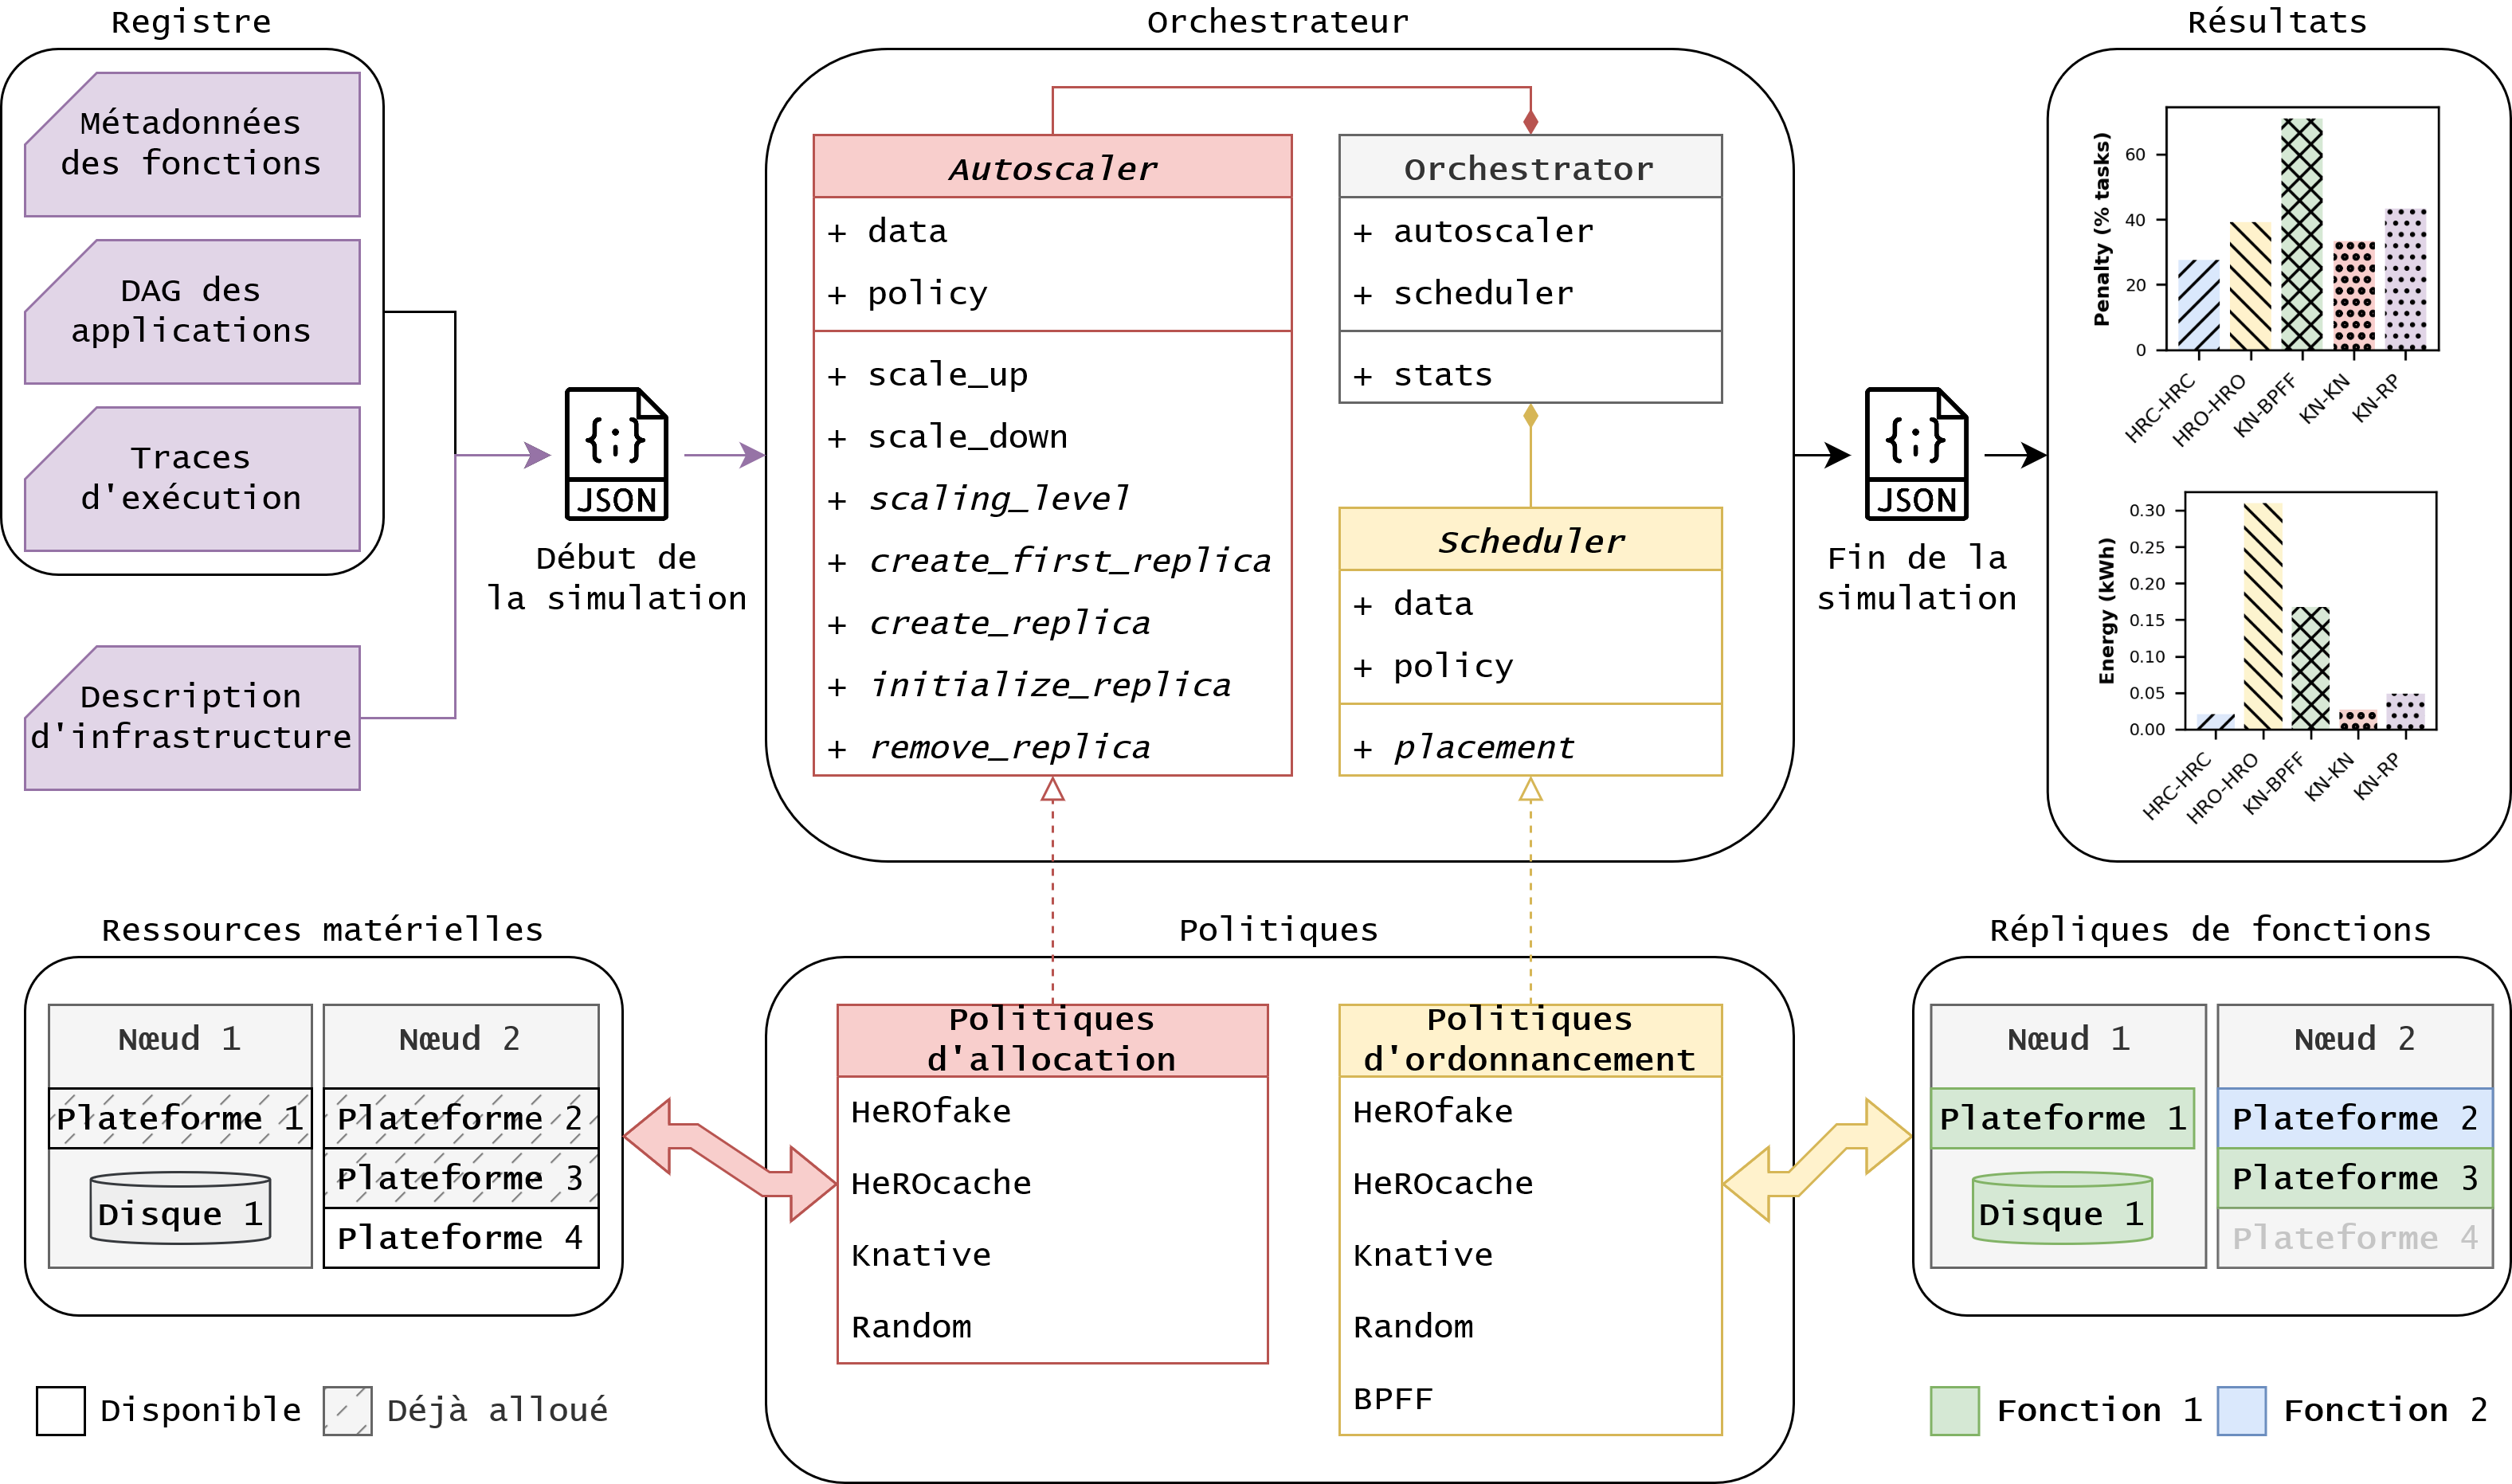
\includegraphics[width=0.8\columnwidth]{img/software-architecture.png}
    \end{center}
\end{frame}

\begin{frame}{HeROsim -- Modèle de coût et validation}
    \begin{columns}
        \column{0.4\textwidth}
        \begin{itemize}
            \item HeROsim est un simulateur à événements discrets ;
            \item L'\textbf{horloge} de la simulation n'avance que sur la base de données préalablement \textbf{mesurées} ;
            \item La précision des estimations dépend de la \textbf{qualité des données d'entrée}.
        \end{itemize}

        \column{0.6\textwidth}
        \begin{center}
            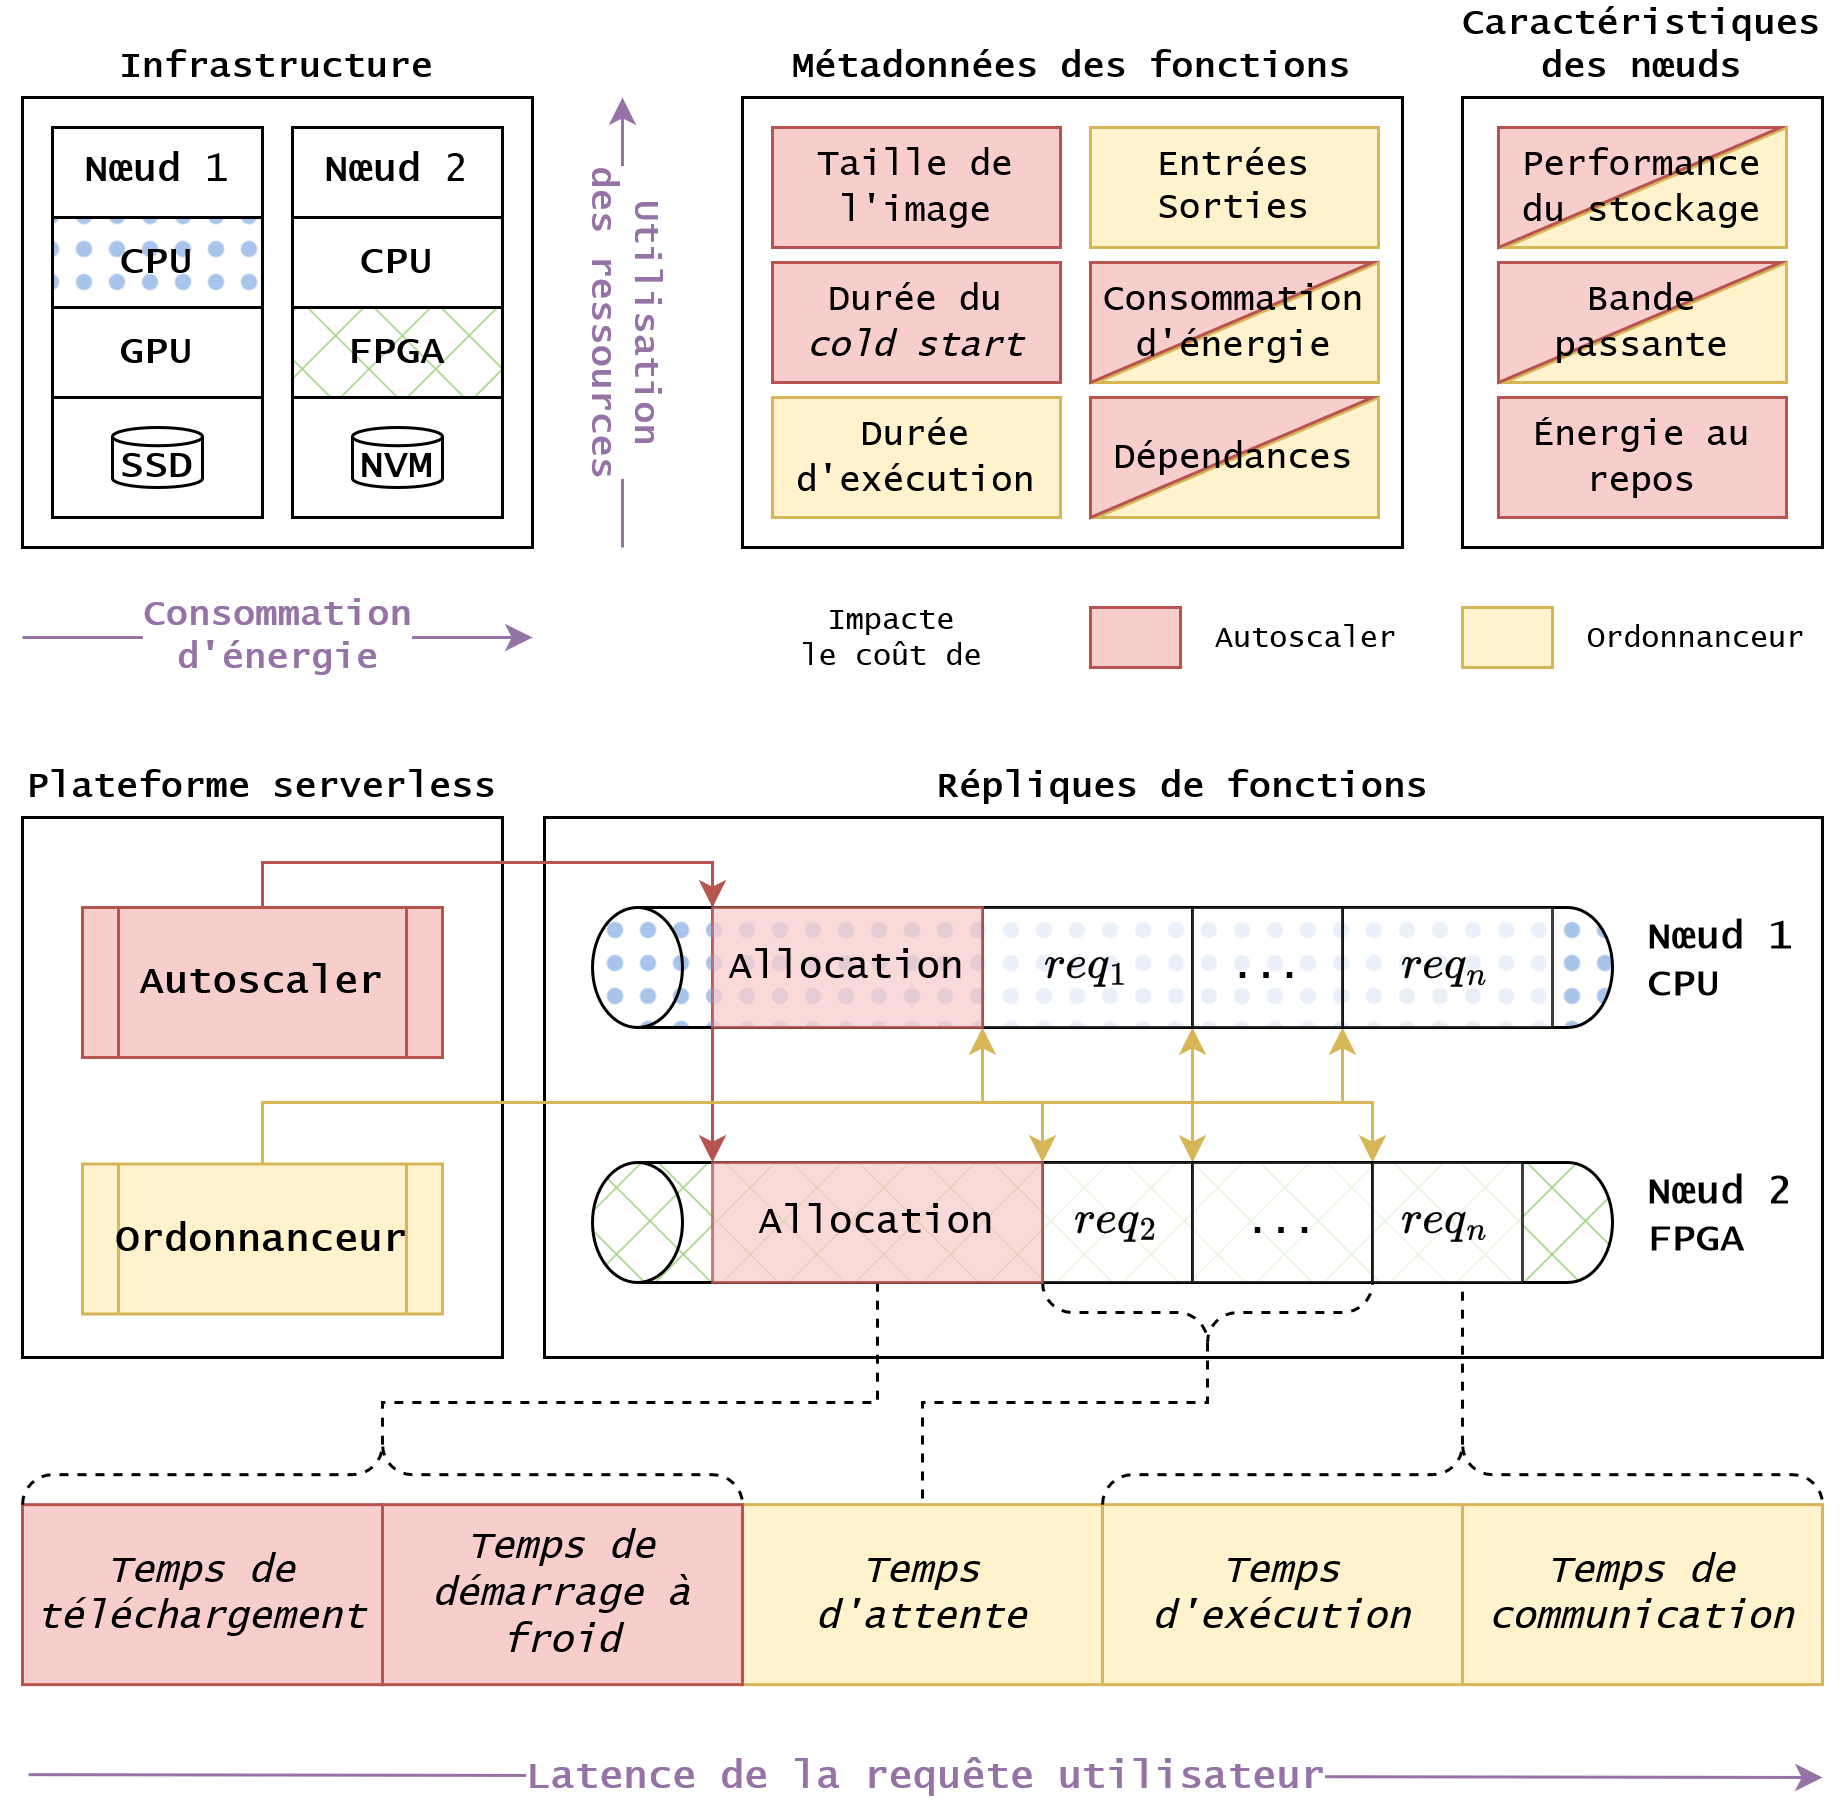
\includegraphics[width=0.8\columnwidth]{img/serverless-cost.png}
        \end{center}
    \end{columns}
\end{frame}

\note[enumerate]{
    \item Les données (caractérisations, traces, infrastructures) de nos deux cas d'étude sont également disponibles sur le dépôt Git, ce qui permet d'évaluer de nouvelles politiques et de comparer leur performance sur les mêmes scénarii.
}

\begin{frame}{HeROsim -- Conclusion}
    \begin{itemize}
        \item HeROsim est disponible sous licence libre~\footnote{\href{https://github.com/b-com/HeROsim}{https://github.com/b-com/HeROsim}} ;
        \item Artefacts pour HeROcache :
        \begin{itemize}
            \item mis en œuvre dans HeROsim ;
            \item soumis à \textit{CCGrid'24} : trois badges de reproductibilité IEEE~\footnote{\href{https://www.niso.org/standards-committees/reproducibility-badging}{https://www.niso.org/standards-committees/reproducibility-badging}} :
            \begin{itemize}
                \item \textit{Open Research Objects} (ORO) ;
                \item \textit{Reusable/Research Objects Reviewed} (ROR) ;
                \item \textbf{\textit{Results Reproduced}} (ROR-R) ;
            \end{itemize}
        \end{itemize}
        \item Soumission au journal \textit{IEEE Internet Computing} (\textit{Special Issue on Serverless Computing}).
    \end{itemize}
\end{frame}

\section{Conclusion}

\begin{frame}{Conclusion -- Résumé des contributions}
    \begin{itemize}
        \item Le cloud est un environnement hautement hétérogène :
        \begin{itemize}
            \item Opportunité : optimisation ;
            \item Menaces : incertitude, coûts d'opportunité ;
        \end{itemize}
        
        \item Approche par \textbf{prédiction des performances} des applications pour l'orchestration serverless :
        \begin{itemize}
            \item Réduction des démarrages à froid pour des fonctions dont les durées d'initialisation dominent les temps d'exécution ;
            \item Accélération des phases d'initialisation par la mise en cache des images de fonctions ;
            \item Minimisation des temps de communication inter-fonctions par la consolidation des applications.
        \end{itemize}

        \item Estimer pour améliorer :
        \begin{itemize}
            \item Proposition d'une méthodologie de caractérisation pour les applications serverless ;
            \item Mise en œuvre d'un simulateur pour évaluer les politiques d'orchestration.
        \end{itemize}
    \end{itemize}
\end{frame}

\begin{frame}{Conclusion -- Perspectives}
    \textbf{Court terme}
    \begin{itemize}
        \item S'affranchir de la phase de caractérisation hors-ligne ;
        \item Formuler le problème de l'ordonnancement pour la dualité prédiction / réaction :
        \begin{itemize}
            \item Prédiction de charge sur séries temporelles ;
            \item Ajustement des seuils de mise à l'échelle par apprentissage renforcé.
        \end{itemize}
    \end{itemize}

    \textbf{Moyen terme}
    \begin{itemize}
        \item Mise à jour du modèle de coût : travaux en cours sur la modélisation de l'impact carbone.
    \end{itemize}

    \textbf{Long terme}
    \begin{itemize}
        \item Orchestration dans le \textit{continuum cloud-edge} :
        \begin{itemize}
            \item Modèle de coût : interférences, pannes, migrations de tâches ;
        \end{itemize}
        \item Stratégies de ralentissement et d'extinction pour un cloud frugal ? Comment éviter l'effet rebond ?
    \end{itemize}
\end{frame}

\begin{frame}[standout]
    Merci de votre attention.
\end{frame}

\appendix

\section{Bibliographie}

\begin{frame}[allowframebreaks]{Références}
    \printbibliography[heading=none]
\end{frame}

\appendix

\section{Annexes}

\begin{frame}{Contributions -- Cas d'usage et généricité applicative}
    \begin{center}
        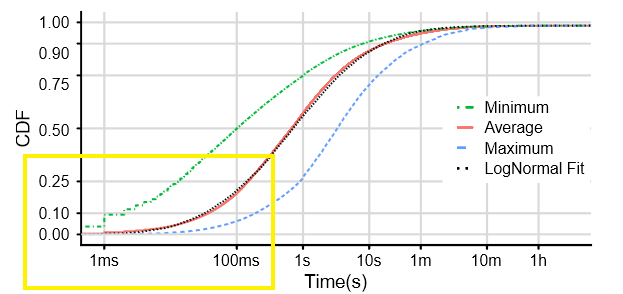
\includegraphics[width=0.7\columnwidth]{img/cdf_short_lived.png}
    \end{center}

    \footnotetext{\fullcite{shahradServerlessWildCharacterizing}}
\end{frame}

\note[enumerate]{
    \item Limite pour les tâches de longue durée : phase de caractérisation hors-ligne
    \item Services dorsaux : a priori, difficile en serverless. Toutefois, des efforts notamment industriels dans ce sens (SQLite chez Fly.io, Postgres distribué...)
}

\begin{frame}{HeROfake -- Niveaux de QoS}
    \begin{columns}
        \column{0.5\textwidth}
        Facteurs de dégradation du temps de réponse (jusqu'à 16x) dans le cloud~\footnote[frame]{\fullcite{nikouniaHypervisorNeighborsNoise2015}} :
        \begin{itemize}
            \item Traversée des couches réseau ;
            \item Partage des ressources (\textit{noisy neighbour}) ;
            \item Surcharge de la virtualisation.
        \end{itemize}

        \column{0.5\textwidth}
        \begin{center}
            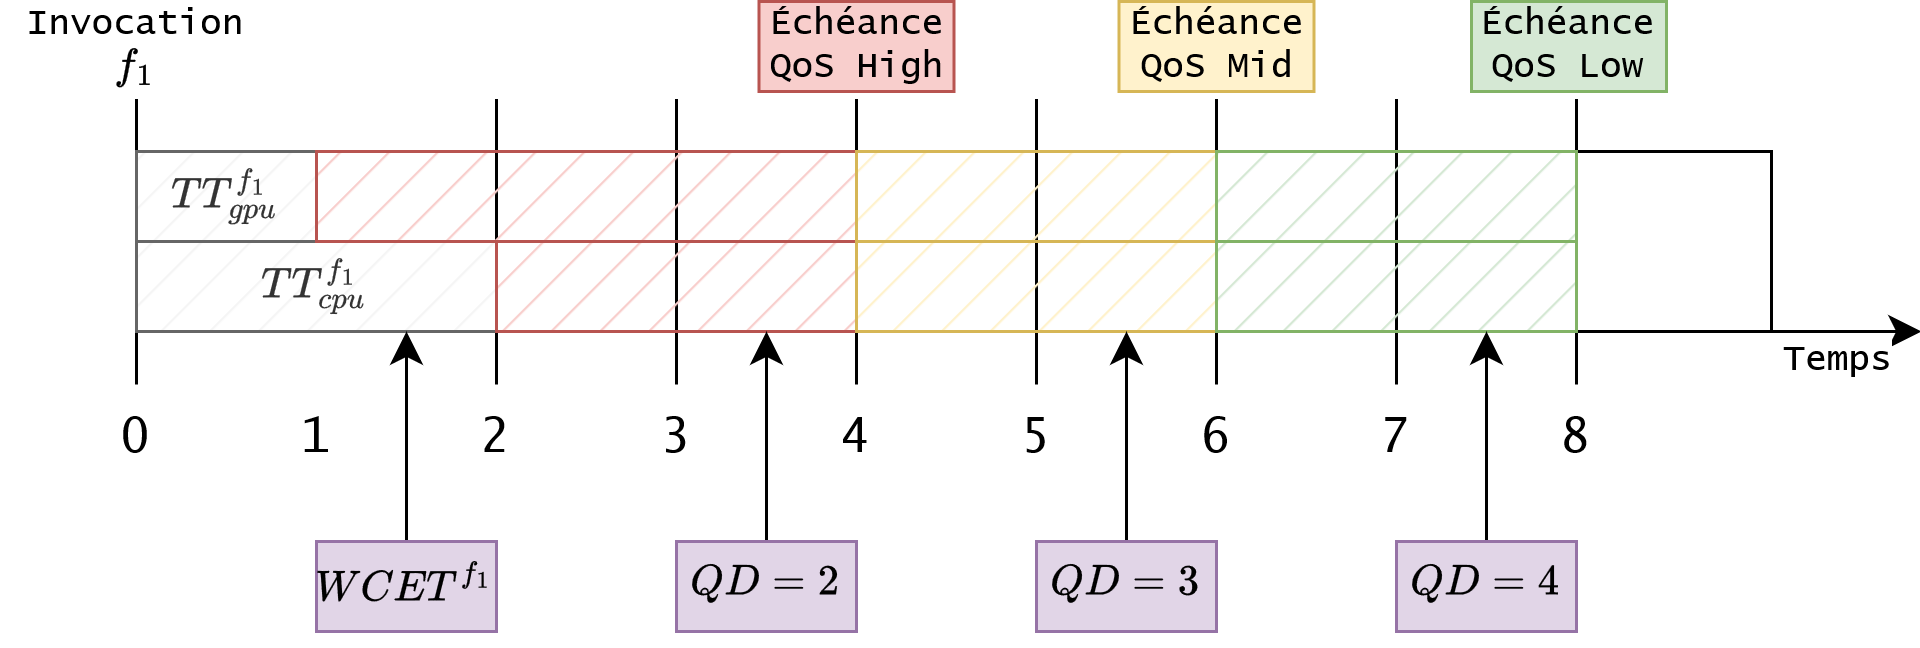
\includegraphics[width=\columnwidth]{img/herofake-scheduling.png}
        \end{center}

        \begin{equation*}
            QP_{f_{N, P}} =
            \begin{cases}
                1 & \text{si} \quad TT_{f_{N, P}} \cdot QD_{f_{N, P}} > WCET_{f} \\
                0 & \text{si} \quad TT_{f_{N, P}} \cdot QD_{f_{N, P}} \leq WCET_{f}
            \end{cases}
        \end{equation*}
    \end{columns}
\end{frame}

\begin{frame}{HeROcache -- Dépendances entre fonctions}
    \begin{columns}
        \column{0.5\textwidth}
        \begin{equation*}
            \begin{split}
                \forall (N, P) \in R_{f}, \, &schedCost_{{f}_{{i}_{N, P}}} = \\
                  &k_{QP} \cdot {QP}_{{f}_{N, P}} \\
                + &k_{EC} \cdot {EC}_{{f}_{N, P}} \\
                + &k_{TC} \cdot {TC}_{{f}_{N, P}}
            \end{split}
        \end{equation*}

        Minimisation des pénalités dans les chaînes de fonctions :

        \begin{equation*}
           QP_{a} = \, \sum_{i = 0}^{F_a} TT_{{f}_{{i}_{N, P}}} > \sum_{i = 0}^{F_a} WCET_{f_{i}} \cdot QD_{a}
        \end{equation*}

        \column{0.5\textwidth}
        Calcul de la consolidation pour maximiser l'utilisation des plateformes :

        \begin{equation*}
            PU_{f_{N, P}} = \frac{Q_{N, P}}{threshold_{f, P}}
        \end{equation*}

        Minimisation :

        \begin{equation*}
            TC_{{f}_{N, P}} = \, exp(PU_{f_{N, P}})
        \end{equation*}
    \end{columns}
\end{frame}

\begin{frame}{HeROcache -- Cache de fonctions}
    Pour une application $a$, calcul de la proportion d'images de ses fonctions déjà en cache sur le nœud :
    
    \begin{equation*}
        \forall f \in a, \, CF_{a}^{{f}_{i_{N, P}}} = \frac{\sum_{i = 0}^{Fa} isCached(f_{i}, N, P)}{F_{a}}
    \end{equation*}

    \textbf{Pré-chargement} des fonctions du DAG de l'application pour améliorer la proportion de fonctions en cache :
    
    \begin{equation*}
        \forall N, \forall P \in N, \, {CP}_{{a}_{N}} = \, \frac{A}{\sum_{i = 0}^{F_{a}} CF_{a}^{{f}_{i_{N, P}}}}
    \end{equation*}
\end{frame}


\begin{frame}[fragile]{HeROsim -- Modéliser des applications}
    \begin{columns}
        \column{0.3\textwidth}
        \begin{minted}[fontsize=\footnotesize]{json}
  "hello-world": {
    "name": "hello-world",
    "dag": {
      "hello": [],
      "world": ["hello"]
    }
  }
        \end{minted}

        \column{0.3\textwidth}
        \begin{minted}[fontsize=\scriptsize]{json}
  "hello": {
    "name": "hello",
    "platforms": [
      "exampleCpu"
    ],
    "memoryRequirements": {
      "exampleCpu": 0.0015
    },
    "coldStartDuration": {
      "exampleCpu": 0.002
    },
    "executionTime": {
      "exampleCpu": 8.5e-3
    },
    "energy": {
      "exampleCpu": 5.5-9
    },
    "imageSize": {
      "exampleCpu": 0.003
    },
    "stateSize": {
      "hello-world": {
        "input": 0,
        "output": 6
      }
    }
  }
        \end{minted}

        \column{0.3\textwidth}
        \begin{minted}[fontsize=\scriptsize]{json}
  "world": {
    "name": "world",
    "platforms": [
      "exampleCpu"
    ],
    "memoryRequirements": {
      "exampleCpu": 0.0030
    },
    "coldStartDuration": {
      "exampleCpu": 0.004
    },
    "executionTime": {
      "exampleCpu": 8.5e-3
    },
    "energy": {
      "exampleCpu": 5.5-9
    },
    "imageSize": {
      "exampleCpu": 0.003
    },
    "stateSize": {
      "hello-world": {
        "input": 6,
        "output": 12
      }
    }
  }
        \end{minted}
    \end{columns}
\end{frame}

\end{document}
